\documentclass{report}

\usepackage{geometry}
\geometry{a4paper,total={170mm,257mm},left=20mm,top=20mm}
\usepackage[utf8]{inputenc}
\usepackage{amsmath}
\usepackage{amsfonts}
\usepackage{amsthm}
\usepackage{amssymb}
\usepackage{bm}
\usepackage{graphicx}
\usepackage{paralist}
\usepackage[dvipsnames]{xcolor}
\usepackage{caption}
\usepackage{subcaption}
\usepackage{hyperref}
\hypersetup{urlbordercolor=ForestGreen,linkbordercolor=RoyalPurple}
\usepackage{tikz}
\usetikzlibrary{positioning}
\usetikzlibrary{intersections}
\usepackage{algpseudocode}
\usepackage{algorithm}
\usepackage{titling}
\usepackage{pgfplots}
\usepackage{fontawesome5}
 % Use the same header and libraries.
%%% Tento soubor obsahuje definice různých užitečných maker a prostředí %%%
%%% Další makra připisujte sem, ať nepřekáží v ostatních souborech.     %%%

%%% Drobné úpravy stylu

% Tato makra přesvědčují mírně ošklivým trikem LaTeX, aby hlavičky kapitol
% sázel příčetněji a nevynechával nad nimi spoustu místa. Směle ignorujte.
\makeatletter
\def\@makechapterhead#1{
  {\parindent \z@ \raggedright \normalfont
   \Huge\bfseries \thechapter. #1
   \par\nobreak
   \vskip 20\p@
}}
\def\@makeschapterhead#1{
  {\parindent \z@ \raggedright \normalfont
   \Huge\bfseries #1
   \par\nobreak
   \vskip 20\p@
}}
\makeatother

% Toto makro definuje kapitolu, která není očíslovaná, ale je uvedena v obsahu.
\def\chapwithtoc#1{
\chapter*{#1}
\addcontentsline{toc}{chapter}{#1}
}

% Trochu volnější nastavení dělení slov, než je default.
\lefthyphenmin=2
\righthyphenmin=2

% Zapne černé "slimáky" na koncích řádků, které přetekly, abychom si
% jich lépe všimli.
\overfullrule=1mm

%%% Makra pro definice, věty, tvrzení, příklady, ... (vyžaduje baliček amsthm)

\theoremstyle{plain}
\newtheorem{veta}{Věta}
\newtheorem{lemma}[veta]{Lemma}
\newtheorem{tvrz}[veta]{Tvrzení}

\theoremstyle{plain}
\newtheorem{definice}{Definice}
\newtheorem*{pozor}{Pozorování}
\newtheorem*{cvic}{Cvičení}
\newtheorem*{fakt}{Fakt}

\theoremstyle{remark}
\newtheorem*{dusl}{Důsledek}
\newtheorem*{pozn}{Poznámka}
\newtheorem*{prikl}{Příklad}

\theoremstyle{plain}
\newtheorem{thm}{Theorem}
%\newtheorem{lemma}[thm]{Lemma}
\newtheorem{claim}[thm]{Claim}

\theoremstyle{plain}
\newtheorem{defn}{Definition}
\newtheorem*{observ}{Observation}
\newtheorem*{exerc}{Exercise}
\newtheorem*{fact}{Fact}

\theoremstyle{remark}
\newtheorem*{cor}{Corollary}
\newtheorem*{rem}{Remark}
\newtheorem*{example}{Example}


%%% Prostředí pro důkazy

\newenvironment{dukaz}{
  \par\medskip\noindent
  \textit{Důkaz}.
}{
\newline
\rightline{$\qedsymbol$}
}

\newenvironment{myproof}{
	\par\medskip\noindent
	\textit{Proof}.
}{
	\newline
	\rightline{$\qedsymbol$}
}


%%% Prostředí pro sazbu kódu, případně vstupu/výstupu počítačových
%%% programů. (Vyžaduje balíček fancyvrb -- fancy verbatim.)

\DefineVerbatimEnvironment{code}{Verbatim}{fontsize=\small, frame=single}

%%% Prostor reálných, resp. přirozených čísel
\newcommand{\R}{\mathbb{R}}
\newcommand{\N}{\mathbb{N}}
\newcommand{\Z}{\mathbb{Z}}

%%% Užitečné operátory pro statistiku a pravděpodobnost
\DeclareMathOperator{\pr}{\textsf{P}}
\DeclareMathOperator{\E}{\textsf{E}\,}
\DeclareMathOperator{\var}{\textrm{var}}
\DeclareMathOperator{\sd}{\textrm{sd}}

%%% Příkaz pro transpozici vektoru/matice
\newcommand{\T}[1]{#1^\top}

%%% Vychytávky pro matematiku
\newcommand{\goto}{\rightarrow}
\newcommand{\gotop}{\stackrel{P}{\longrightarrow}}
\newcommand{\maon}[1]{o(n^{#1})}
\newcommand{\abs}[1]{\left|{#1}\right|}
\newcommand{\dint}{\int_0^\tau\!\!\int_0^\tau}
\newcommand{\isqr}[1]{\frac{1}{\sqrt{#1}}}

%%% Vychytávky pro tabulky
\newcommand{\pulrad}[1]{\raisebox{1.5ex}[0pt]{#1}}
\newcommand{\mc}[1]{\multicolumn{1}{c}{#1}}


% set up \maketitle to accept a new item
\predate{\begin{center}\placetitlepicture\large}
	\postdate{\par\end{center}}

% commands for including the picture
\newcommand{\titlepicture}[2][]{%
	\renewcommand\placetitlepicture{%
		\includegraphics[#1]{#2}\par\medskip
	}%
}
\newcommand{\placetitlepicture}{} % initialization

 % Use global macros.

\usepackage{babel}

%%% Specific for this paper.
\newcommand{\overrightsimarrow}[1]{\mathrel{\overset{\leadsto}{#1}}}

\title{Kombinatorika a grafy}
\author{Tomáš Turek}
\titlepicture[width=3in]{res/tree.pdf}
\date{\today}

\begin{document}
	\maketitle
	
	\INFO{There are my notes from three courses on combinatorics and graph theory. First two are in czech and the last one is in english. The first part is missing almost all of its proofs.}
	
	\tableofcontents
	\part{Kombinatorika a grafy I}
	\chapter{Odhady}

\section{Odhady faktoriálu}

Faktoriál: $n \in \mathbb{N}: n!$. Poskládání $n$ prvků.

\begin{tvrz}
	$\forall n \in \mathbb{N}: n^{n/2} \leq n! \leq n^n$
\end{tvrz}

\begin{dukaz}
	Horní odhad se dá napsat jako: $n! = \prod_{i=1}^{n}i \leq \prod_{i=1}^{n} n = n^{n}$. Dolní odhad použijeme, že $i(n+1 - i) \geq n$ (to platí pro $i=1$ a $i=n$). Potom pro $2 \leq i \leq \lceil \frac{n}{2} \rceil$ máme $i(n+1-i) \geq 2 \frac{n}{2} = n$. Obdobný odhad je i pro $\lceil \frac{n}{2} \rceil \leq i \leq n$. Následně $(n!)^2 = n1 \cdot n2 \dots 2(n-1) \cdot 1n \geq n^{n}$. Potom platí, že $n! \geq n^{n/2}$.
\end{dukaz}

\begin{veta}
	$\forall n \in \mathbb{N}: e (\frac{n}{e})^n \leq n! \leq en(\frac{n}{e})^n$
\end{veta}

\begin{dukaz}
	Horní odhad: Pro $n = 1$ platí $(1 = 1! \leq e 1 \left( \frac{1}{e} \right)^{1} = 1)$. Nechť $n \geq 2$.
	
	$$
	n! = n (n-1)! \leq n e (n-1)\left( \frac{n-1}{e} \right)^{n-1} = e n \left( \frac{n}{e} \right)^{n}e \left( \frac{n-1}{n} \right)^{n} - \left( \frac{n-1}{n} \right)^{n} =
	$$
	
	$$
	= e \left( 1 - \frac{1}{n} \right)^{n} \leq e \left( e^{\frac{-1}{n}} \right)^{n} = 1
	$$
	
	Dolní odhad: Pro $n = 1$ platí $(1 = \left( \frac{1}{n} \right)^{1} \leq 1! = 1)$. Nechť $n \geq 2$.
	
	$$
	n! = n(n-1)! \geq n e \left( \frac{n-1}{e} \right)^{n-1} = e \left( \frac{n}{e} \right)^{n} e \left( \frac{n-1}{n} \right)^{n-1} - \left( \frac{n-1}{n} \right)^{n-1} \geq 1
	$$
	
	$$
	\Updownarrow
	$$
	
	$$
	\frac{1}{e} \left( \frac{n}{n-1} \right)^{n-1} \leq 1
	$$
	
	$$
	\frac{1}{e} \left( \frac{n}{n-1} \right)^{n-1} = \frac{1}{e} \left( 1 + \frac{1}{n-1} \right)^{n-1} \leq \frac{1}{e} \left( e^{\frac{1}{n-1}} \right)^{n-1}
	$$
\end{dukaz}

\begin{lemma}
	$1+x \leq e^x$
\end{lemma}

\begin{dukaz}
	$f(x) := e^x - (x+1)$ chceme ukázat, že $f(x) \geq 0$ pro $\forall x \in \mathbb{R}$. $f'(x) = e^x - 1 \Rightarrow (f'(x) = 0 \Leftrightarrow x = 0)$. $f''(x) = e^x$. $f''(x) = 1 > 0 \Rightarrow$ v bodě $x = 0$ je globální minimum pro $f \Rightarrow f(x) \geq 0$ pro $\forall x \in \mathbb{R}$.
\end{dukaz}

\begin{veta}[Stirlingův vzorec]
	$n! \approx n \sqrt{2\pi n} (\frac{n}{e})^n$ $\lim_{n \to \infty} \frac{n!}{\sqrt{2\pi n}(\frac{n}{e})^n} = 1$
\end{veta}

\section{Binomický koeficient}

Počet $k$-prvkových podmnožin $n$-prvkových množin: 

$$
n,k \in \mathbb{N}: \binom{n}{k}=\frac{n!}{k!(n-k)!}
$$

\begin{pozor}
	\begin{enumerate}
		\item $\forall n,k \in \mathbb{N}: (\frac{n}{k})^k \leq \binom{n}{k} \leq n^k$
		\item největší prvek $\binom{n}{\lceil \frac{n}{2} \rceil} = \binom{n}{\lfloor \frac{n}{k} \rfloor}$
	\end{enumerate}	
\end{pozor}

\begin{dukaz}
	Empty.
\end{dukaz}

\subsection{Binomická věta}

$$
\frac{2^{2m}}{2m+1} \leq \binom{2m}{m} \leq 2^{2m}
$$

\begin{veta}
	$\forall m \in \mathbb{N}: \frac{2^{2m}}{2\sqrt{m}} \leq \binom{2m}{m} \leq \frac{2^{2m}}{\sqrt{2m}}$
\end{veta}

Užití Stirlingového vzorce: $\binom{2m}{m} \approx \frac{2^{2m}}{\sqrt{\pi m}}$. $\forall k,n \in \mathbb{N}: n > k, \binom{n}{k} \leq (\frac{en}{k})^k$.

\begin{dukaz}
	Empty.
\end{dukaz}

\subsection{Aplikace (náhodné procházky)}

$n$ kroků a v každém bodě mám $50\%$ že půjdu doprava anebo doleva. Střední hodnota počtu návratů do $0$. $X$ - počet návratů do $0$. $A_{2n}=$ jev po $2n$ krocích se dostanu do $0$. $X = \sum_{n=1}^{\infty} I_{A_{2n}}$. $\Pr[A_{2n}]=\frac{\binom{2n}{n}}{2^2n}$.

$$
\mathbb{E}[X] = \mathbb{E}[\sum_{n=1}^{\infty}I_{A_{2n}}] = \sum_{n=1}^{\infty} \mathbb{E} [I_{A_{2n}}] = 
$$

$$
= \sum_{n=1}^{\infty} Pr [I_{A_{2n}}] = \sum_{n=1}^{\infty} \frac{\binom{2n}{n}}{2^2n} \geq \sum_{n=1}^{\infty} \frac{1}{2\sqrt{n}} = \infty
$$
	\chapter{Vytvořující funkce}

Početní metoda, kde spojitými funkcemi vyjadřujeme posloupnosti.

\begin{definice}
	Pro posloupnost $(a_{i})_{i=0}^{\infty}$ je mocninnou řadou $a(x) = \sum_{i=0}^{\infty}a_{i}x^{i}$.
\end{definice}

Posloupnost lze převést na funkci, ale při převodu nazpátek je třeba aby posloupnost nerostal moc rychle.

\begin{prikl}
	\begin{enumerate}
		\item $a_i = 1$ pokud $0 \leq i \leq n$ jinak $a_i = 0$. Tedy $(a_i)_{i=0}^{\infty}=(1,\dots,1,0,0,\dots)$. Potom funkce je $\frac{1-x^{n+1}}{1-x}$ z geometrické řady.
		\item $\forall i: a_i = 1$ to je potom nekonečná geometrická řada, takže je to $\frac{1}{1-x}$.
		\item $a_i = \binom{n}{i}$ potom funkce vychází z binomické věty, takže je $(1+x)^{n}$.
	\end{enumerate}
\end{prikl}

\begin{tvrz}
	Pokud pro $(a_i)_{i=0}^{\infty} \exists k \in \mathbb(R)$ takové, že $\forall i: |a_i| \leq k^i$, pak pro všechna $x \in (\frac{-1}{k}, \frac{1}{k})$ řada $a(x) = \sum_{i=0}^{\infty}a_ix^i$ konverguje absolutně a na libovolném $\epsilon$ okolí 0 určuje i $koeficienty_a$, protože $i_a = \frac{a^{(i)}(0)}{i!}$.
\end{tvrz}


Obecný postup:

\begin{enumerate}
	\item kombinatorický objekt s neznámým počtem
	\item vytvořující funkce
	\item rozklad na vytvořující funkce se známými koeficienty
	\item určení hodnoty
\end{enumerate}


\begin{table}[!h]\centering
	\begin{tabular}{| l | l | l |}
		\hline
		Operace & Posloupnosti & Funkce \\
		\hline
		Součet                   & $(a_0+b_0, a_1+b_1, \dots)$                        & $(a+b)(x) = \sum_{i=0}^{\infty}(a_i+b_i)x^i$ \\
		$\alpha$-násobek         & $(\alpha a_0, \alpha a_1, \dots)$                  & $\alpha a(x) = \sum_{i=0}^{\infty}(\alpha a_i)x^i$ \\
		Posun vpravo o $n$ pozic & $(0,0,\dots ,a_0, a_1, \dots)$                     & $x^na(x)\sum_{i=0}^{\infty}a_ix^{i+n}$ \\
		Posun vlevo o $n$ pozic  & $(a_n, a_{n+1}, dots )$                            & $\sum_{i=0}^{\infty}(a_{i+n}x^i = \frac{a(x) - \sum_{i=0}^{\infty}a_ix^i}{x^n}$ \\
		Dosazení $\alpha x$      & $(a_0, \alpha a_1, \alpha^2 a_2, \dots)$           & $a(\alpha x) = \sum_{i=0}^{\infty}a_i+ \alpha^i x^i$ \\
		Dosazení $x^n$           & $(a_0, 0, \dots, 0, a_1, 0, \dots)$ & $a(x^n) = \sum_{i=0}^{\infty}a_ix^ni$ \\
		Derivace                 & $(a_1, 2a_2, 3a_3, \dots)$                         & $a'(x) = \sum_{i=1}^{\infty}ia_ix^{i-1}$ \\
		Integrál                 & $(0, a_0, \frac{a_1}{2}, \frac{a_2}{3}, \dots)$    & $\int_{0}^{x} a(x) \mathtt{d} x = \sum_{i=0}^{\infty}\frac{a_i}{i+1}x^{i+1}$ \\
		Součin                   & $(c_0, c_1, c_2, \dots)$                           & $a(x)b(x) = \sum_{i=0}^{\infty}(c_i)x^i$ \\
		\hline
	\end{tabular}
\end{table}

\section{Řešení rekurentních rovnic}

Ukázka na Fibonacciho čísle. Určíme $F_n$ jako koeficient funkce $F(x)=\sum_{i=0}^{\infty}F_ix^i$. Máme $F_{n+2} = F_{n+1} + F_{n}, \forall n\geq 0$. \textbf{Vynásobíme rovnici $x^n$:} $F_{n+2} x^n= F_{n+1} x^n + F_{n} x^n$.\textbf{Sčítáme přes $n \geq 0$:} $\sum_{n \geq 0} F_{n+2} x^n= \sum_{n \geq 0} F_{n+1} x^n + \sum_{n \geq 0} F_{n} x^n$ to se rovná:

$$
\frac{F(x)-F_0 - F_1}{x^2} = \frac{F(x)-F_0}{x} +F(x)
$$

teď určíme

$$
F(x) = \frac{x}{1-x-x^2} = \frac{x}{(1 - \frac{1 + \sqrt{5}}{2}x)(1 - \frac{1 - \sqrt{5}}{2}} = \frac{\frac{1}{\sqrt{5}}}{1 - \frac{1 + \sqrt{5}}{2}x} - \frac{\frac{1}{\sqrt{5}}}{1 - \frac{1 - \sqrt{5}}{2}x}
$$

to už lze převést

$$
F_n = \frac{1}{\sqrt{5}}\left[ \left( \frac{1+\sqrt{5}}{2} \right)^n - \left( \frac{1-\sqrt{5}}{2} \right)^n \right]
$$

to je tzv. \textbf{Binetův vzorec}. Tento postup funguje pro všechny \textbf{Homogenní lineární rekurence $k$-tého stupně s konstantními koeficienty}, tedy typu:

$$
a_{n+k} = \alpha_{k-1}a_{n+k-1} + \dots + \alpha_0 a_n, k \in \mathbb{N}, \alpha_{k-1}, \dots, \alpha_0 \in \mathbb{R}
$$

\section{Aplikace vytvořujících funkcí}

Nadefinujeme zobecněnou \textbf{binomickou větu} pro

$$
n \in \mathbb{R}, r \in \mathbb{Z}_{0}^{+}: \binom{n}{r}:= \frac{n(n-1)(n-2)\dots(n-r+1)}{r!},
$$

speciálně $\binom{n}{0}=1$.

\begin{veta}[Zobecněná binomická věta]
	$\forall r \in \mathbb{R}$ je $(1+x)^r$ vytvořující funkcí posloupnosti $\left( \binom{r}{0}, \binom{r}{1}, \binom{r}{2}, \dots \right)$ a řada $\sum_{i=0}^{\infty}\binom{r}{i}x^{i}$ konverguje pro $\forall x \in (-1, 1)$.	
\end{veta}

\begin{dukaz}
	Empty.
\end{dukaz}

\begin{dusl}
	$\forall n \in \mathbb{N} \ \forall x \in (-1,1)$ platí $\frac{1}{(1-x)^{n}}=\sum_{i=0}^{\infty}\binom{n+i-1}{n-1} x^{i}$.
\end{dusl}

\begin{dukaz}
	Empty.
\end{dukaz}

\section{Aplikace - Catalanova čísla}

\textbf{Zakořeněný binární strom} - buď je prázdný, nebo obsahuje speciální vrchol zvaný \textbf{kořen} a pár zakořeněných stromů, které tvoří \textbf{levý} a \textbf{pravý podstrom}.

$b_{n}$ = počet bin. zak. stromů na $n \in \mathbb{N}_{0}$ vrcholech, potom $b(x) = \sum_{n = 0}^{\infty}b_{n} x^{n}$ je příslušná vytvořující funkce.

\begin{veta}
	Pro každé $n \in \mathbb{N}_{0}$ platí $b_{n}=\frac{1}{n+1}\binom{2n}{n}$. Kde se $\frac{1}{n+1}\binom{2n}{n}$ značí jako $C_n$ a říká se mu n-té \textbf{Catalanovo číslo}.
\end{veta}

\begin{dukaz}
	Empty.
\end{dukaz}

Catalanova čísla mají mnoho interpretací, například počet triviálních uzávorkování s $n$ páry závorek anebo počet triangulací.
	\chapter{Konečně projektivní roviny (KPR)}

Jistá nová struktura, která je velice symetrická a vzácná. Jedná se o množinový systém (\textbf{hypergraf} - zobecnění grafu, kde hrany mohou být k-tice. Využívá se v samoopravných kódech a přichází z geometrie.

\section{Eukleidovy axiomy}

\begin{enumerate}
	\item každé 2 body určují přímku
	\item každou úsečku lzze prodloužit na přímku
	\item ze zadaného bodu lze opsat kružnici procházejícím druhým zadaným bodem
	\item všechny pravé úhly jsou stejné
	\item bodem lze k přímce vést právě 1 rovnoběžku
\end{enumerate}

\begin{definice}[KPR]
	Konečná množina $\mathcal{X}$ a systém $\mathcal{P}$ podmnožin $\mathcal{X}$ tvoří KPR $(\mathcal{X}, \mathcal{P})$ = (body, přímky) pokud splňuje tyto tři axiomy:
	
	\begin{enumerate}
		\item $\forall x,y \in \mathcal{X}, x \neq y, \exists !P \in \mathcal{P}: \{x,y\} \subseteq P$
		\begin{itemize}
			\item každé 2 body určují právě jednu přímku
		\end{itemize}
		\item $\forall P,Q \in \mathcal{P}, P \neq Q: |P \cap Q| = 1$
		\begin{itemize}
			\item každé 2 přímky se protínají právě v 1 bodě
		\end{itemize}
		\item $\exists C \subseteq \mathcal{X}, |C| = 4, \forall P \in \mathcal{P}: |C \cap P| \leq 2$
		\begin{itemize}
			\item existují 4 body v obecné poloze
		\end{itemize}
	\end{enumerate}
\end{definice}

Jako příklad je \textbf{Fanova rovina}, která má 7 přímek a 7 bodů. Jak lze vidět na obrázku \ref{fans-plane}.

\begin{figure}[!h]\centering
	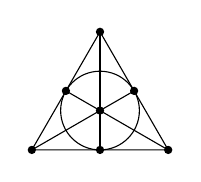
\begin{tikzpicture}
		\draw (0,0) circle (0.5);
		\draw (90:1) -- (-30:1)--(210:1)--cycle;
		\draw (90:1)--(0,0);
		\draw (210:1)--(0,0);
		\draw (-30:1)--(0,0);
		\draw (30:0.5)--(0,0);
		\draw (150:0.5)--(0,0);
		\draw (270:0.5)--(0,0);
		\fill (-0.866,-0.5) circle (1.5pt);
		\fill (0.866,-0.5) circle (1.5pt);
		\fill (0,-0.5) circle (1.5pt);
		\fill (0,1) circle (1.5pt);
		\fill (0,0) circle (1.5pt);
		\fill (0.433,0.25) circle (1.5pt);
		\fill (-0.433,0.25) circle (1.5pt);
	\end{tikzpicture}
	\caption{Fanova rovina}
	\label{fans-plane}
\end{figure}

\begin{tvrz}
	V KPR obsahuje každá přímka stejný počet bodů. $\forall P,Q \in \mathcal{P} |P|=|Q|$.
\end{tvrz}

\begin{dukaz}
	Empty.
\end{dukaz}

\begin{definice}
	Řád projektivní roviny: $(\mathcal{X}, \mathcal{P})$ je $|P|-1$ pro $P \in \mathcal{P}$.
\end{definice} 

\begin{tvrz}
	Je-li $(\mathcal{X}, \mathcal{P})$ KPR řádu $n$, pak platí:
	
	\begin{enumerate}
		\item každým bodem prochází právě $n+1$ přímek
		\item $|\mathcal{X}| = n^{2} + n + 1$
		\item$|\mathcal{P}| = n^{2} + n + 1$
	\end{enumerate}
\end{tvrz}

\begin{dukaz}
	Empty.
\end{dukaz}

\section{Dualita KPR}

"Přechod z přímek na body a z bodů na přímky."

\begin{definice}
	\textbf{Duální množinový systém} k množinovému systému $(\mathcal{X}, \mathcal{P})$ je $(\mathcal{P}, \{ \{P \in \mathcal{P} : x \in P \}: x \in \mathcal{X} \})$, zkráceně \textbf{duál}
\end{definice}

\begin{tvrz}
	Duálem KPR řádu $n$ je KPR řádu $n$.
\end{tvrz}

\begin{dukaz}
	Empty.
\end{dukaz}

\section{Existence KPR}

Kromě Fanovy roviny zatím neznáme žádné další příklady konečných projektivních rovin. Ale samozřejmě se ví o dalších které existují jmenovitě pro $(2,3,4,5,7,8,9,11)$ a $12$ už se neví. Domněnka je, že KPR řádu $n$ existuje $\Leftrightarrow$ $n$ je mocnina prvočísla. Nicméně je to pořád otevřené.

\begin{veta}
	Pokud existuje algebraické těleso o $n$ prvcích, potom existuje KPR řádu $n$.
\end{veta}

\begin{dukaz}
	Empty.
\end{dukaz}

Konstrukce funguje nad každým tělesem a například nad $\mathbb{R}$ dává \textbf{reálnou projektivní rovinu}.

\section{Latinský čtverec}

\begin{definice}
	Latinský čtverec řádu $n \in \mathbb{N}$ je tabulka $n \times n$ čísel z $\{ 1, \dots, n\}$, ve které se žádné číslo neopakuje v žádném řádku ani sloupci.
\end{definice}

\subsection{Ortogonalita}

\begin{definice}
	Latinský čtverce $L, L'$ stejného řádu jsou \textbf{ortogonální}, pokud pro každé $l, l' \in \{ 1, \dots , n\}$ existují $i,j \in \{ 1, \dots , n\}$, takové že $L_{ij} = l, L'_{ij}=l'$. Zapisuje se jako $L  \perp L'$.
\end{definice}

\begin{pozor}
	Pro ortogonální latinské čtverce $L, L'$ řádu $n$ a pár $(l,l') \in \{ 1, \dots , n\} \times \{ 1, \dots , n\}$ je pozice $(l,l')$ s $L_{ij}=l, L'_{ij}=l'$ určena jednoznačně.
\end{pozor}

\begin{dukaz}
	Počet párů $(l,l')$ je $n^{2}$, stejně jako počet párů $(i,j)$.
\end{dukaz}

\begin{pozor}
	Je-li $L = (L_{ij})_{i,j = 1}^n$ latinský čtverec a $\Pi : \{ 1, \dots , n\} \to \{ 1, \dots , n \}$ perm, tak potom $\Pi (L) := (\Pi (L_{ij})_{i,j =1}^n$ je latinský čtverec stejného řádu.
\end{pozor}

\begin{dukaz}
	$\Rightarrow$ BŮNO první řádek je vžzdy vzestupná řada. $\Rightarrow$ Je-li $L \perp L'$, pak $\Pi (L) \perp L'$.
\end{dukaz}

\begin{dusl}
	Počet \textbf{navzájem ortogonálních} nanejvýš čtverců řádu $n \in \mathbb{N}$ je $n-1$.
\end{dusl}

\begin{dukaz}
	Empty.
\end{dukaz}

\begin{veta}
	Konečná projektivní rovina řádu $n \geq 2$ existuje $\Leftrightarrow$ existuje $n-1$ navzájem ortogonálních latinských čtverců řádu $n$.
\end{veta}

\begin{dukaz}
	Empty.
\end{dukaz}
	\chapter{Toky v sítích}

\begin{definice}
	Síť je čtveřice $(G, z, s, c)$, kde $G = (V, E)$ je orientovaný graf (tedy $V \subseteq V \times V$), $z \in V$ je \textbf{zdroj}, $s \in V$ je \textbf{stok} ($z \neq s$) a $c: E \to \mathbb{R}_{0}^{+}$. Hodnotu $c(e)$ nazýváme \textbf{kapacitou} hrany $e \in E$.
\end{definice}

\begin{definice}
	Tok v síti $(G = (V, E), z, s, c)$ je $f: E \to \mathbb{R}_{0}^{+}$ splňující následující podmínky:
	
	\begin{enumerate}
		\item $\forall r \in E : 0 \leq f(e) \leq c(e)$ (velikost toku je omezená kapacitou)
		\item \textbf{Kirchhoffův zákon} co přitéká do vrcholu, musí odtéct, neboli:
	\end{enumerate}
	
	$$
	\forall u \in V \setminus \{ z, s\}: \sum_{v:(u,v) \in E} f(u,v) - \sum_{v:(v, u) \in E} f(v,u) = 0
	$$
\end{definice}

\begin{definice}
	\textbf{Velikost toku} $f$ je $w(f) = \sum_{v:(z,v) \in E} f(z,v) - \sum_{v:(v, z) \in E} f(v,z)$.
\end{definice}

\begin{tvrz}
	Pro každou síť existuje maximální tok.
\end{tvrz}

\begin{dukaz}[Náčrt]
	Z analýzy víme, že spojitá funkce na kompaktní množině nabývá maxima. Množina $\mathcal{F} \subseteq \mathbb{R}^{|E|}$ všech toků je kompaktní funkce $w: \mathcal{F} \to \mathbb{R}$ je spojitá.
\end{dukaz}

\begin{definice}
	Řez v síti $(G, z, s, c)$ je $R \subseteq E$ taková, že každá orientovaná cesta ze zdroje $z$ do stoku $s$ používá aspoň jednu hranu z $R$.
\end{definice}

Speciálně hrany vycházející ze $z$ či hrany vycházející do $s$ tvoří řez.

\begin{definice}
	\textbf{Kapacita řezu} $R$ je $c(R) = \sum_{e \in R}c(e)$.
\end{definice}

Řezu je jen konečně mnoho $\Rightarrow$ jistě existuje řez minimální kapacity.

\begin{veta}[hlavní věta o tocích]
	Velikost maximálního toku = kapacita minimálního řezu, nebo-li, pro každou síť platí: $\max \ w(f) = \min \ c(R)$, kde $f$ je tok a $R$ řez.
\end{veta}

\begin{definice}[Elementární řez]
	Pro $A \subseteq V$, kde $z \in A$ a $s \notin A$, nazveme množinu $R_A = \{ e = (u,v) \in E: u \in A, v \notin A\}$ \textbf{elementárním řezem}. Opravdu se jedná o řez, protože pokaždé su musí nějak opustit $A$.
\end{definice}

\begin{pozor}
	Každý řez $R$ obsahuje elementární řez.
\end{pozor}

\begin{dukaz}
	Zvolme $A$ jako množinu vrcholů dosažitelných po orientované cestě ze zdroje v grafu $(V, E \setminus R)$. Potom $z \in A, s \notin A$, protože $R$ je řez $\Rightarrow R_A$ existuje $(u,v) \in R_A \Leftrightarrow u \in A, v \notin A \Rightarrow (u,v) \in R$, tedy $R_A \subseteq R$.
\end{dukaz}

\begin{pozor}
	Každý \textbf{v inkluzi minimální} řez $R$ je elementární. Nebo-li $R \setminus \{ e \}$ není řezem pro $\forall e \in R$.
\end{pozor}

\begin{dukaz}
	Z předchozího pozorování musí $R$ obsahovat elementární řez $R_A \subseteq R$ a z minimality platí $R_A = R$.
\end{dukaz}

\begin{lemma}
	Je-li $f$ tok a $R_A$ elementární řez, pak platí:
	
	$$
	w(f) = \sum_{u \in A, v \notin A, (u,v) \in E}f(u,v) - \sum_{u \in A, v \notin A, (v, u) \in E} f(v,u)
	$$
\end{lemma}

\begin{dukaz}
	Empty.
\end{dukaz}

\begin{dukaz} (Věty)
	Empty.
\end{dukaz}

\section{Fordův-Fulkersonův algoritmus}

\begin{algorithmic}[1]
	\State Nastav $f(e) = 0$ pro $\forall e \in E$
	\While {$\exists$ zlepšující cesta $P$}
	\State  vylepšuj po ní tok o $\epsilon_P$
	\EndWhile\\
	\Return Stávající tok $f$
\end{algorithmic}

\begin{veta}[o celočíselnosti]
	Jsou-li kapacity celočíselné, pak F.F. najde max. tok po konečně mnoha krocáích a navíc má takový tok celočíselnou velikost.
\end{veta}

\begin{dukaz}
	Tok se vždy zlepší o celé číslo $\epsilon_P >$ a $w(f) < \infty$.
\end{dukaz}

Existují sítě s iracionálními kapacitami, kde F.F nenajde maximální tok a nekonverguje k výsledku. V síti s celočíselnými kapacitami má F.F. alg. časovou složitost $O(w(f)(|V|+|E|))$, kde $f$ je tok. Takže je to v čase $O(|V|+|E|)$. Pokud bychom specifikovali výběr zlepšující cesty na nejkratší dostaneme \textbf{Edmondsův-Karpův algoritmus}, který má časovou složitost $0(|V|+|E|^2)$.

\section{Königova-Egerváryho věta}

\begin{definice}
	V grafu $G = (V,E)$ nazveme množinu $C \subseteq V$ \textbf{vrcholovým pokrytím}, pokud $C \cap e \neq \emptyset$ pro $\forall e \in E$.
\end{definice}

Zjistit minimální velikost vrcholové pokrytí je NP-těžká úloha.

\begin{definice}
	\textbf{Párováním} v $G$ je podgraf tvořený disjunktními hranami.
\end{definice}

\begin{veta}(Königova-Egerváryho věta)
	V bipartitiním grafu je velikost min. vrcholového pokrytí rovna velikosti maximálního párování (do počtu hran).
\end{veta}

\begin{dukaz}
	Empty.
\end{dukaz}

\section{Hallova věta}

\begin{definice}
	Mějme konečné množiny $X$ a $I$. \textbf{Množinový systém} $\mathcal{M}$ je $(M_{i}: i \in I)$, kde $M_{i} \subseteq X$. \textbf{Systém ruzných reprezentantů (SRR)} pro $\mathcal{M}$ je prosté zobrazení $f: I \to X$ takové, že $\forall i \in I : f(i) \in M_{i}$. Tedy $f$ je výběr jednoho prvku z každé $M_{i}$ takový, že žádný prvek nevybereme víckrát. \textbf{Incidenční graf} systému $\mathcal{M}$ je bipartitní graf $G_{\mathcal{M}}=(I \cup X, E)$, kde $E = \{ \{ i,x\}: i \in I, x \in X, x \in M_{i} \}$. Pokud $\mathcal{M}$ má SSR $\Leftrightarrow$ $S_{\mathcal{M}}$ obsahuje párování velikosti $|I|$.
\end{definice}

\begin{veta}[Hallova věta]
	$\mathcal{M}$ má SSR $\Leftrightarrow \forall J \subseteq I: |\cup_{j \in J}M_{j}| \geq |J|$. Pravé části se říká \textbf{Hallova podmínka}, také se věta označuje jako \textbf{Hall's marriage theorem}.
\end{veta}

\begin{definice}
	Empty.
\end{definice}


S axiomem výběru by šlo dokázat variantu s konečnými $M_{i}$ a nekonečnými $I,X$. S nekonečnými $I,X$ to platit nemusí.

\section{Rozšiřování latinských obdélníků}

\begin{dusl}
	V každém bipartitním grafu $G =  (A \cup B, E)$ s $E \neq \emptyset$ a $\mathtt{deg}_{G}(x) \geq \mathtt{deg}_{G}(y)$ pro každé $x \in A, y \in B$ existuje párování velikosti $|A|$.
\end{dusl}

\begin{dukaz}
	Empty.
\end{dukaz}

Latinský obdélník typu $k \times n$ pro $k \leq n$ je tabulka s řádky s $n$ sloupci vyplněnými symboly $1, \dots, n$ tak, že se v žádném řádku ani sloupci žádný symbol neopakuje.

\begin{veta}
	Každý latinský obdélník typu $k \times n$ lze doplnit na latinský čtverec řádu  $n$.
\end{veta}

\begin{dukaz}
	Empty.
\end{dukaz}
	\chapter{Míra souvislosti grafu}

\begin{definice}
	Graf je \textbf{souvislý} pokud jsou každé dva vrcholy spojené cestou, jinak je graf \textbf{nesouvislý} a je rozložen na aspoň dvě \textbf{komponenty souvislosti}.
\end{definice}

Nyní budeme zkoumat jak moc je graf odolný proti rozpadnutí po odebrání hrany nebo vrcholu.

\begin{definice}
	\textbf{Hranovým řez} v grafu $G = (V,E)$ je množina hran $F \subseteq E$ taková, že graf $G - F = (V, E \setminus F)$ je nesouvislý. (Také se někdy nazývá jako \textbf{separátor}.)
\end{definice}

\begin{definice}
	\textbf{Vrcholovým řezem} v grafu $G = (V,E)$ je množina vrcholů $A \subseteq V$ taková, že graf $G - A = (V \setminus A, E \cap \binom{V \setminus A}{2})$ je nesouvislý.
\end{definice}

\begin{definice}
	\textbf{Hranová souvislost} grafu $G = (V,E)$ je
	
	$$
	k_{e}(G) =
	\left\{
	\begin{array}{ll}
		\min\{|F|: F \text{ je hranový řez v }G \} \\
		k_{e}(G) = 1 \text{ pokud } G \equiv K_{1}
	\end{array}
	\right.
	$$
\end{definice}

\begin{definice}
	\textbf{Vrcholová souvislost} grafu $G = (V,E)$ je
	
	$$
	k_{v}(G) =
	\left\{
	\begin{array}{ll}
		\min\{|A|: A \text{ je vrcholový řez v }G \} \\ 
		k_{v}(G) = 1 \text{ pokud } G \equiv K_{1} \\
		k_{v}(G) = n-1 \text{ pokud } G \equiv K_{n}, n \geq 2
	\end{array}
	\right.
	$$
\end{definice}

Nesouvislé grafy mají vrcholovou i hranobvou souvislost 0. 

\begin{definice}
	Pro $r \in \mathbb{N}_{0}$ je graf \textbf{hranově $r$-souvislý}, pokud $k_{e}(G) \geq r$.
\end{definice}

\begin{definice}
	Pro $r \in \mathbb{N}_{0}$ je graf \textbf{vrcholově $r$-souvislý}, pokud $k_{v}(G) \geq r$.
\end{definice}

\begin{pozor}
	$\forall G = (V,E), G \neq K_{1}: k_{e}(G), k_{v}(G) \leq \min \{ \mathtt{deg}_{G}(v), v \in V \}$
\end{pozor}

\begin{lemma}
	$\forall G = (V,E) \forall e \in E: k_{e}(G) -1 \leq k_{e}(G-e) \leq k_{e}(G)$ Po odebrání hrany klesne hranová souvislost maximálně o 1.
\end{lemma}

\begin{dukaz}
	Empty.
\end{dukaz}

\begin{lemma}
	$\forall G = (V,E) \ \forall e \in E: k_{v}(G) -1 \leq k_{v}(G-e) \leq k_{v}(G)$ Po odebrání hrany klesne vrcholová souvislost maximálně o 1.
\end{lemma}

\begin{dukaz}
	Empty.
\end{dukaz}

\begin{dusl}
	$\forall G=(V,E): k_{v}(G) \leq k_{e}(G)$ Vrcholová souvislost je maximálně stejná jako hranová souvislost.
\end{dusl}

\begin{dukaz}
	Empty.
\end{dukaz}

Nerovnost může být ostrá. To lze vidět na příkaldu "motýlka". Lze vidět na obrázku \ref{motylek}.

\begin{figure}[!h]\centering
	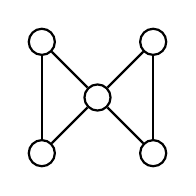
\begin{tikzpicture}[node distance={10mm}, thick, main/.style = {draw, circle}]
		\node[main] (1) {};
		\node[main] (2) [below right of=1] {};
		\node[main] (3) [below left of=1] {};
		\node[main] (4) [above right of=1] {};
		\node[main] (5) [above left of=1] {};
		\draw (1) -- (2);
		\draw (1) -- (3);
		\draw (1) -- (4);
		\draw (1) -- (5);
		\draw (4) -- (2);
		\draw (5) -- (3);
	\end{tikzpicture}
	\label{motylek}
	\caption{Graf "motýlek".}
\end{figure}

\begin{veta}[Ford-Fulkersonova věta]
	$\forall G \ \forall t \in \mathbb{N}: k_{e} \geq t \Leftrightarrow$ mezi každými $2$ vrcholy grafu $G$ $\exists$ $\geq t$ hranově disjunktních cest.
\end{veta}

\begin{dukaz}
	Empty.
\end{dukaz}

Varianat Fordovy-Fulkersonovy věty platí i pro vrcholovou souvislost. Tyto věty jsou známé také jako Mengerovy věty.

\begin{veta}[Mengerova věta]
	$\forall G \ \forall t \in \mathbb{N}: k_{e}(G) \geq t \Leftrightarrow$ mezi každými $2$ vrcholy grafu $G$ $\exists$ $\geq t$ vrcholově disjunktních cest (mimo $u,v$).
\end{veta}

\begin{dukaz}
	Empty.
\end{dukaz}

Jelikož lze zjistit tok maximální velikost v polynomiálním čase, tak máme algoritmus na zjištení $k_{e}(G), k_{v}(G)$ také v polynomiálním čase.

\section{2-souvislost podrobněji}

\begin{definice}
	Hranový řez velikosti $1$ se nazývá \textbf{most} a vrcholový řez velikosti  $1$ se nazývá \textbf{artikulace}.
\end{definice}

Pro graf $G=(V,E)$ s $e \in E$ označme $C \div e$ graf vzniklýz $G$ operací \textbf{podrozdělení hrany} $e$ na cestu délky $2$.

\begin{lemma}
	Pro každý graf $G=(V,E)$ a pro každou hranu $e \in E$ platí: $G$ je vrcholově $2$-souvislý $\Leftrightarrow G \div e$ je vrcholově $2$-souvislý.
\end{lemma}

\begin{dukaz}
	Empty.
\end{dukaz}

\begin{veta}[Ušaté lemma]
	Graf $G$ je vrcholově $2$-souvislý $\Leftrightarrow G$ lze vytvořit z $K_{3}$ operacemi přidávání a podrozdělování hran. Proč "Ušaté lemma"? Přidání hrany a její podrozdělení odpovídám přidání cesty mezi 2 vrcholy (="přiepení ucha").
\end{veta}

\begin{veta}[Alternativní znění]
	$G$ je vrcholově $2$-souvislý $\Leftrightarrow G$ lze vytvořit z cyklu přidá-\newline váním uší, protože přidávání ucha lze symulovat přidáním hrany a jejím podrozdělení.
\end{veta}

\begin{dukaz}
	Empty.
\end{dukaz}
	\chapter{Počítání dvěma způsoby}

Metoda důkazů v kombinatorice. Určíme nějaký neznámý počet $X$ vyjádřením počtu $Z$ dvěma výrazy, z nichž jeden $X$ obsahuje a druhý ne $\Rightarrow$ máme vyjádření pro $X$.

\section{Cayleyho vzorec}

Kolika způsoby lze vytvořit strom na vrcholech $\{ 1, \dots , n \}$? Nebo-li jaká je počet koster $\kappa (n)$ grafu $K_{n}$? 

\begin{definice}
	Kostra grafu $G = (V, E)$ je strom $T = (V, E')$ s $E' \subseteq E$.
\end{definice}


\begin{veta}[Cayleyho vzorec]
	Pro každé $n \geq 1$ platí $\kappa (n) = n^{n-2}$.
\end{veta}

Existuje řada důkazů s velmi odlišnými myšlenkami, ukážeme si nejjednodušší založený na počítání dvěma způsoby.

\begin{dukaz}
	Empty.
\end{dukaz}

\begin{veta}
	Graf $K_{n}-e$ má $(n-2)n^{n-3}$ koster pro $n \geq 2$.
\end{veta}

\begin{dukaz}
	Empty.
\end{dukaz}


Počet koster $\kappa (G)$ grafu $G = (\{ 1, \dots , n \}, E)$ lze určit pomocí determinantu. Uvažme \textbf{Laplacián $L(G)$} grafu $G$, tedy matici $L(G) = (L_{ij})_{i,j=1}^{\infty}$, kde

$$
L_{ij} =
\left\{
\begin{array}{ll}
	\mathtt{deg}_{G}(i) \text{ pokud } i=j \\
	-1 \text{ pokud } (i,j) \in E \\
	0 \text{ jinak }
\end{array}
\right.
$$

\begin{veta}[Kirchhoffova věta]
	$\forall G : \kappa (G) = \det (L(G)^{1,1})$, kde $(L(G)^{1,1})$ je Laplacián $L(G)$ bez 1. řádků a 1. sloupce.
\end{veta}

\section{Spernerova věta}

\begin{definice}
	Systém $\mathcal{M} \subseteq 2^{ \{ 1, \dots , n \} }$ podmnožin $n$-prvkové množiny $\{ 1, \dots , n \}$ je \textbf{nezá-\newline vislý}, pokud platí: $\forall A, B \in \mathcal{M}, A \neq B: A \nsubseteq B \land A \nsupseteq B$.
\end{definice}

\begin{veta}[Spernerova věta]
	Každý nezávislý systém v $2^{ \{ 1, \dots , n \} }$ obsahuje $\leq \binom{n}{\lceil \frac{n}{2}\rceil}$ množin a tento odhad je těsný. Ekvivalentně: Nejdelší antiřetězec v $(2^{ \{ 1, \dots , n \} }, \leq)$ má právě $\binom{n}{\lceil \frac{n}{2}\rceil}$ prvků.
\end{veta}

\begin{dukaz}
	Empty.
\end{dukaz}
	\chapter{Úvod do Ramseyovy teorie}

"Každý velký systém obsahuje homogenní podsystém" dané velikosti.

\begin{definice}
	\textbf{Obarvení} množiny $X$ $r$ barvami (zkráceně $r$-obarvení) je libovolné zobraze-\newline ní přiřazující každému prvku z $X$ jednu z $r$ barev.
\end{definice}

\begin{veta}[Dirichletův princip, Pigeonhole principle]
	$\forall r, n_{1}, \dots , n_{r} \in \mathbb{N}$: obarvíme-li prvky množiny $X$ $r$ barvami, pak je-li $|X| \geq 1+ \sum_{i = 1}^{r}(n_{i} - 1)$, $X$ obsahuje $n_{i}$ prvků $i$-té barvy.
\end{veta}

\begin{dukaz}
	Triviální.
\end{dukaz}

Co kdybychom chtěli obarvit dvojice?

\begin{definice}
	Pro $k,l \in \mathbb{N}$ buď $R(k,l)$ nejmenší $N \in \mathbb{N}$ takové, že každé $2$-obarvení \textit{(BÚNO: červené a modré obarvení)} $E(K_{N})$ obsahuje červené $K_{k}$ nebo modré $K_{l}$ jako podgraf.
\end{definice}

\begin{veta}[Ramseyova věta pro $2$ barvy]
	$\forall k,l \in \mathbb{N}: R(k,l)$ je konečné. Dokonce $R(k,l) \leq \binom{k+l-2}{k-1} = \binom{k+l-2}{l-1}$.
\end{veta}

\begin{dukaz}
	Empty.
\end{dukaz}

Určit Ramseyovská čísla $R(k,l)$ přesně je velice obtížné (už pro malé případy). Známá čísla $R(3,3) = 6$, $R(4,4) = 18$.

\begin{veta}
	$\forall k \geq 3: R(k,k) > 2^{k/2}$
\end{veta}

\begin{dukaz}
	Empty.
\end{dukaz}

Rozšíření Ramseyovy věty na více barev a také na barvení $p$-tic vrcholů.

\begin{definice}
	Pro čísla $p,r,n_{1}, \dots , n_{r} \in \mathbb{N}$ ($p$ - velikost barevných množin, $r$ - počet barev, $n_{i}$ - velikost 1-barevných podstruktur, které chceme najít) definujeme **Ramseyovo číslo** $R_{p}(n_{1}, \dots , n_{n})$ jako nejmenší $N \in \mathbb{N}$ takové, že pro každou množinu $X$ s $|X| \geq N$ a každé $r$-obarvení množiny $\binom{X}{p}$ existuje $i \in \{ 1, \dots , n \}$ a $Y \subseteq X$ takové, že $|Y_{i}| = n_{i}$ a všechny $p$-tice z $\binom{Y}{p}$ mají $i$-tou barvu.
\end{definice}

\begin{veta}[Ramseyova věta pro $p$-tice]
	Pro každé $p,r,n_{1}, \dots , n_{n}$ je $R_{p}(n_{1}, \dots , n_{n})$ konečné.
\end{veta}

\begin{dukaz}
	Empty.
\end{dukaz}

\section{Aplikace - Erdösova-Szekeresova věta}

\begin{definice}
	$P$ = konečná množina bodů v rovině $\mathbb{R}^{2}$. $P$ je v \textbf{obecné poloze}, pokud neobsahuje 3 body na přímce. $P$ je v \textbf{konvexní poloze}, pokud tvoří množinu vrcholů konvexního mnohoúhelníku.
\end{definice}

\begin{lemma}
	Každá množina 5 bodů v $\mathbb{R}^{2}$ v obecné poloze obsahuje 4 body v konvexní poloze.
\end{lemma}

\begin{dukaz}
	Empty.
\end{dukaz}

\begin{veta}[Erdösova-Szekeresova věta]
	Pro každé $r \in \mathbb{N}$ existuje nejmenší $ES(r) \in \mathbb{N}$ takové, že každá konečná množina s $\geq ES(r)$ body v $\mathbb{R}^{2}$ b obecné poloze obsahuje $r$ bodů v konvexní poloze.
\end{veta}

\begin{dukaz}
	Empty.
\end{dukaz}

Erdösova-Szekeresova domněnka je že $\forall r \geq 2: ES(r) = 2^{r-2}+1$. Zatím se zná, že to je dolní odhad a horní jako $\leq 2^{r+o(r)}$.

\begin{veta}[Nekonečná verze Ramseyovy věty]
	Pro každé $p,r \in \mathbb{N}$ a pro každé $r$-obarvení množiny $\binom{\mathbb{N}}{p}$ existuje nekonečná $A \subseteq \mathbb{N}$ taková, že všechny její $p$-tice mají v daném $r$-obarvení stejnou barvu.
\end{veta}

\begin{dukaz}
	Empty.
\end{dukaz}

Nekonečná verze implikuje konečnou. Dá se dokázat sporem, my si ji ukážeme pro $n_{1} = \dots = n_{n} = n$.

\begin{lemma}[Königovo lemma]
	V každém zakořeněném stromě, který má nekonečně mnoho vrcholů ale jen konečné stupně existuje nekonečná cest začínající v kořeni.
\end{lemma}

\begin{dukaz}(implikace konečné věty)
	Empty.
\end{dukaz}

	\chapter{Samoopravné kódy}

\begin{definice}
	\textbf{Abeceda} $\Sigma$ = konečná množina symbolů, \textbf{slovo} délky $n$ = posloupnost $n$ symbolů, $\Sigma^n$ = množina všech slov délky $n$.
\end{definice}

\begin{definice}
	\textbf{Hammingova vzdálenost}: $x,y \in \Sigma^n : d(x,y) = |{i \in \{1,\dots ,n\}: x_i \neq y_i}|$, neboli počet pozic, kde se $x$ a $y$ liší. $d$ je metrika a tedy $(\Sigma^n, d)$ je metrický prostor.
\end{definice}

\begin{definice}
	\textbf{(Blokový) kód} je $C \subseteq \Sigma^n$ a prvky $C$ jsou \textbf{kódova slova}. Pomocí $C$ umíme opravit $\leq t$ chyb, pokud $\forall y \in \Sigma^n \exists \text{nanejvys 1 slovo} x \in C \text{t.ž.} d(x,y)\leq t$.
\end{definice}

\begin{definice}
	Parametry kódu:
	
	\begin{enumerate}
		\item délka = $n$,
		\item velikost abecedy $q = |\Sigma|$,
		\item dimenze $k = \log_q|C|$,
		\item vzdálenost $d = \min_{x, x' \in C, x \neq x'} d(x, x')$. 
	\end{enumerate}
	
	Kód s parametry $n,k,d,q$ značíme $(n,k,d)_q$.
\end{definice}

V kódu s parametry $(n,k,d)_q$ dokážeme opravit $\leq \lfloor \frac{d-1}{2} \rfloor$ chyb. Množiny slov ve vzdálenosti $\leq \lfloor \frac{d-1}{2} \rfloor$ od kódových slov jsou navzájem disjunktní. Pokud $d \leq n$, tak dokážeme opravit $\leq \lfloor \frac{n-1}{2} \rfloor$.

\begin{prikl}
	\begin{enumerate}
		\item opakovací kód: každý symbol $n$-krát zopakujeme, paramtery: $(n, 1, n)_q$
		\item charakteristický vektory KPR
		\begin{itemize}
			\item kódová slova $P$ - $\{0,1\}$ - vektor, kde na pozici $x$ je $1 \leftrightarrow x \in P$
			\item $(X, \mathcal{P})$ - KPR řádu $n$
			\item parametry: $(n^2 + n + 1, \log_{2} (n^2+n+1), 2n)_{2}$
			\item $|X| = n^2+n+1$ a $|C|=|\mathbb{P}| = n^2+n+1$
			\item $d = 2n$
			\item 2 kódove slova sdílí jednu jedničku, na zbytku se liší na $2n$ pozicích 
		\end{itemize}
		\item hadamardovy kódy
		\begin{itemize}
			\item hadamardova matice řádu $n$ je $H \in \{-1, 1\}$, kde $H \cdot H^T = n \cdot I_n$
			\item každý 2 různy řádky se liší na $n/2$ pozicích
			\item zvolme $C=\{\text{řádky} H\} \cup \{-\text{řádky}H\}$
			\item parametry: $(n, 1+\log_2(n), \frac{n}{2})_2$
		\end{itemize}
	\end{enumerate}
	
	$$
	H_1 = 1
	$$
	
	$$
	H_2 =
	\begin{pmatrix}
		1 & 1 \\
		1 & -1
	\end{pmatrix}
	$$
\end{prikl}

Sylvestrova konstrukce hadamardovy matice:

$$
H_{n+1} = 
\begin{pmatrix}
	H_n & H_n \\
	H_n & - H_n
\end{pmatrix}
$$

\textbf{Hadamardova domněnka:} pro $\forall k \in \mathbb{N} \exists \text{ hadamardova matice řádu } 4k$

Kódy $C, C'$ jsou ekvivalentní, pokud se liší jen pořadím pozic. $\exists \Pi \in S_n: X = (x_1, \dots, x_n) \in C \leftrightarrow \Pi(X) = (X_{\Pi(1), \dots, X_{\Pi(n)} \in C}$. Pro jaké parametry existuje kód?

\begin{definice}
	Kombinatorická koule je středem $X \in \Sigma^n$ a poloměrem $t$ je $B(X,t) = \{y \in \Sigma^n : d(x,y) \leq t\}$.
\end{definice}

\begin{lemma}
	Je-li $C$ kód se vzdáleností $2t+1$, pak $\forall X,X' \in C: B(X,t) \cap B(X',t) = \emptyset$.
\end{lemma}

\begin{dukaz}
	Sporem - $\exists z \in B(x, t) \cap B(x', t) \implies d(x, x') \leq d(x,z) + d(x', z) \leq t+t = 2t$, kde $d(x, x')$ je $\geq 2t+1$, takze celkove je $2t+1 \leq 2t$.
\end{dukaz}

\begin{veta}[Hammingův odhad]
	$\forall \text{ kód } C$ s parametrama $(n,k,d)_q$ plati, že $|C| \leq \frac{q^n}{V(t)}$.
\end{veta}

\begin{dukaz}
	$d = 2t +1 \implies$ koule okolo kódovych slov s poloměrem $t$ jsou disjunktní. $\implies |C| \cdot |V(t)| \leq |\Sigma^n| \implies |C| \leq \frac{|\Sigma^n|}{|V(t)|} = \frac{|q^n|}{|V(t)|}$.
\end{dukaz}

\begin{definice}
	\textbf{Perfektní kód} = kód s parametry $(n,k, 2t+1)_q$ a s $|C| = \frac{q^n}{V(t)}$.
\end{definice}


Opakovací kód s $q=2$ a lichou delkou.

\begin{veta}[Gilbertův - Varshalův odhad]
	$\forall n,q,d \in \mathbb{N}: \exists \text{ kód } C$ s parametry $(n,k,d)_q$, kde $|C| \geq \frac{q^n}{V(d-1)}$.
\end{veta}

\begin{dukaz}
	Stačí iterativně odebírat slova z $\Sigma^n$ spolu se slovy v Hammingové vzdálenosti $\leq d-1$. Proces skončí po $\geq \frac{q^n}{V(d-1)}$ krocích, protože odebírané koule jsou nanejvýš disjunktní.
\end{dukaz}

\begin{definice}
	\textbf{Linearní kódy} - jako abecedu použít konečné těleso $\mathbb{K} = \Sigma^n$. Podprostor vektorového prostoru $\mathbb{K}^n$ s parametry $n,k,d,q$ značíme $[n,k,d]_q$.
\end{definice}

\begin{prikl}
	\begin{enumerate}
		\item opakovací kódy nad $\mathbb{Z}_p$ [nejsou linearní]
		\item charakteristický vektory KPR [nejsou linearní]
		\item hadamardovy kódy [obecně ne, ze Sylvestrovy konstrukce ano]
	\end{enumerate}
\end{prikl}

\section{Lineární kódy}

Víme, že každé těleso $\mathbb{K}$ odpovídá Galoisovu tělesu $\mathbb{F}_{q}$. $\forall x,y,z \in \mathbb{K}^{n}: d(x,y) = d(x+z, y+z) = d(x-y,0)$. $\Rightarrow$ minimální vzdálenost $d$ se rovná $\min_{x,y \in C, x \neq y} \{ d(x-y,0) = \min_{x \in C, x \neq 0} \{ d(x,0) \} \}$. $\Rightarrow$ ke zjištění $d$ není třeba zkoumat všechny dvojice, stačí počítat nenulové složky kódových slov. Výhodou lineárních kódů je úsporný popis, namísto všech $q^{r}$ prvků kódu stačí uvést $r$ prvků nějaké jeho báze.

\begin{definice}
	\textbf{Generující matice} kódu $C$ = matice $M \in \Sigma^{r \times n}$ jejíž řádky tvoří bázi kódu $C$. V prostoru $\mathbb{F}_{q}^{n}$ definujeme \textbf{skalární součin} $<x,y> = \sum_{i=1}^{n}x_{i}y_{i}$ pro $x = (x_{1}, \dots , x_{n}), y = (y_{1}, \dots , y_{n}) \in \mathbb{F}_{q}^{n}$. Nejedná se o klasický skalární součin podle klasické definice, protože neplatí $<x,x> = 0 \Leftrightarrow x=0$ (třeba $x = (1,1,0,0)$ nad $\mathbb{F}_{2}^{4}$).
\end{definice}

\begin{definice}
	\textbf{Duálním kódem} k lineárnímu kódu $C$ je jeho ortogonální doplněk.
	
	$$
	C^{\bot} = \{ x \in \mathbb{F}_{q}^{n}: <x,y> = 0 \text{ pro každé } y \in C \}
	$$
\end{definice}



Z povahy našeho skalárního součinu nemusí platit $C \cap C^{\bot} = \{ 0 \}$. Platí $\dim(C^{\bot}) + \dim(C) = n$ a $(C^{\bot})^{\bot} = C$. Generující matice $M^{\bot}$ kódu $C^{\bot}$ se nazývá \textbf{kontrolní matice}. Řádky kontrolní matice určují lineární rovnice, které musí každé slovo z $C$ splňovat (a naopak každý vektor z $\mathbb{F}_{q}^{n}$, který je splňuje, je kódovým slovem v $C$). Nebo-li $C = \{ x \in \mathbb{F}_{q}^{n}: M^{\bot}x = 0 \}$.

Mějme lineární kód $C$ s parametry $[n,r,d]_{q}$.

\subsection{Kódování lineární kódy}

Ze vstupního slova $z \in \mathbb{F}_{q}^{n}$ chceme vytvořit kódové slovo $x \in C \subseteq \mathbb{F}_{q}^{n}$. Nechť $M \in \mathbb{F}_{q}^{r \times n}$ je generující matice kódu $C$. Pro každý lineární kód existuje ekvivalentní kód, jehož generující matice má tvar:

$$
\begin{pmatrix}
	I{r} & B
\end{pmatrix}
$$

Kde výška je $r$ a šířka $n$. Říká se jí \textbf{standardní forma}. Stačí generující matici upravit Gaussovou eliminací a popřípadě zpermutovat sloupce. $\Rightarrow$ BŮNO: Matice $M$ je ve standardní formě. Jako kódové slovo zvolíme $x = M^{\top}z \in C$. $\Rightarrow x$ má na prvních $r$ souřadnicích slovo $z$ (\textbf{indormační symboly}) a na zbylých $n-r$ souřadnicích obsahuje \textbf{kontrolní symboly}.

$$
\begin{matrix}
	&
	\begin{pmatrix}
		z
	\end{pmatrix} \\
	\begin{pmatrix}
		I_{r} \\
		B^{\top}
	\end{pmatrix}
	&
	\begin{pmatrix}
		z \\
		.
	\end{pmatrix}
\end{matrix}
$$

\subsection{Dekódování lineárních kódů}

Po odeslání $x \in C$ bylo přijato $y \in \mathbb{F}_{q}^{n}$. Příjemce zná pouze $y$ a chce najít kódové slovo, které je mu nejblíž. Nechť $M^{\bot}$ je kontrolní matice kódu $C$, pokud je matice $M$ve standardní formě pak:

$$
M^{\bot} =
\begin{pmatrix}
	-B{\top} & I_{n-r}
\end{pmatrix}
$$

kde šířka je $r$ a výška $n-r$, protože pak $M^{\bot} M^{\top} = -B^{\top}I_{r} + I_{n-r}B^{\top}=0$. Jako \textbf{syndrom slova} $y \in \mathbb{F}_{q}^{n}$ nazveme součin $M^{\bot}y$, protože $C = \{ x \in \mathbb{F}_{q}^{n}:M^{\bot}x=0 \}$, tak máme určené lineární zobrazení $S:\mathbb{F}_{q}^{n} \to \mathbb{F}_{q}^{n-r}$ splňující $C = Ker(S)$. Zobrazení $S$ nazveme \textbf{syndrom}. Zobrazení $S$ je na, protože platí $\dim(Ker(S)) + \dim(Im(S)) = \dim(\mathbb{F}_{q}^{n})$, kde $Im(S)$ je obraz $S$.

\begin{lemma}
	Zobrazení $S$ je prosté na $B(0,t)$ kde $t=\lfloor \frac{d-1}{2} \rfloor$.
\end{lemma}

\begin{dukaz}
	Empty.
\end{dukaz}

Podle lemma tedy k $S \restriction B(0,t)$ existuje inverzní zobrazení $S^{-1}: S(B(0,t)) \to B(0,t)$. $S^{-1}$ není lineární, ale jde popsat tabulkou s $q^{n-k}$ prvky z $B(0,t)$ a v této tabulce je pro každý syndrom slova uloženo nějaké slovo s minimální vahou a s daným syndromem.

Co víme:

\begin{enumerate}
	\item Pro $y \in B(x,t)$ máme $S(y-x) = S(y) - S(x) = S(y)$ (díky linearitě a toho že $x \in Ker(S)$). Neboli $y$ a vzniklá chyba $y-x$ mají stejný syndrom.
	\item Pro $y \in B(x,t)$ máme $y-x \in B(0,t)$ a tedy $y-x = S^{-1}(S(y-x))$. Neboli vzniklou chybu jde vyjádřit pomocí $S$.
	\item $x = y - (y - x) = y - S^{-1}(S(y-x)) = y - S^{-1}(S(y))$ nezávisý na $x$, pro dané $y$ pomocí syndromu $S(y)$ dokážeme určit kódové slovo $x$, ze kterého vzniklo, nastalo-li $\leq t$ chyb.
\end{enumerate}


\subsection{Jak dekódovat}

Pro přijaté slovo $y \in \mathbb{F}_{q}^{n}$ spočítat $x = y - S^{-1}(M^{\bot}y)$, kde $M^{\bot}$ je kontrolní matice a zobrazení $S^{-1}$ máme připravené jako tabulku. Nastane-li $\leq t$ chyb, je $x$ kódové slovo, ze kterého $y$ vzniklo.

\begin{tvrz}
	Vzdálenost $d$ kódu $C$ = minimální počet lineárně závislých sloupců kontrolní matice $M^{\bot}$.
\end{tvrz}

\begin{dukaz}
	Víme, že $d$ = minimální počet nenulových symbolů v nenulovém slově $x$ z $C$. $x \in C \Leftrightarrow M^{\bot}x = 0$ tedy sliupce $M^{\bot}$ vybrané nenulovými složkami $x$ jsou lineárně závislé.
\end{dukaz}

\section{Hammingovy kódy}

Příklad lineárních kódů, které jsou dokonce perfektní. Jejich nevýhodou je, že nedokáží opravit příliš mnoho chyb. Například nad tělesem $\mathbb{F}_{2}$. Mějme parametr $r = 3$. Generující matice:

$$
M =
\begin{pmatrix}
	&  &  & - & l_{1} & - \\
	& I_{2^{r}-r-1} &  & - & l_{2} & - \\
	&  &  & - & l_{3} & -
\end{pmatrix}
$$

Kde $l_{i}$ jsou všechny nenulové vektory z $\mathbb{F}_{2}^{r}$ různé od vektorů kanonické báze. Kontrolní matice:

$$
M^{\bot} =
\begin{pmatrix}
	| & | & | &  &  &  \\
	l_{1} & l_{2} & l_{3} &  & I_{r} &  \\
	| & | & | &  &  & 
\end{pmatrix}
$$

Parametry matic jsou $r$ a $2^{r}-r-1$. Dva vektory z $\mathbb{F}_{2}^{r} \setminus \{0\}$ jsou lineárně závislé $\Leftrightarrow$ jsou totožné $\Rightarrow$ minimální počet lineárně závislých sloupců v $M^{\bot}$ je $3$ a podle tvrzení 13.2. je vzdálenost kódu $3$. $\Rightarrow$ jedná se o kód s parametry $[2^{r}, 2^{r}-r-1, 3]_{2}$, takže opraví $\leq 1$ chybu

\begin{prikl}
	Pro  $r=3$ dostaneme kód s parametry $[7,4,3]_{2}$. Jedná se o kód sestavený z Fanovy roviny přidáním počátku a doplňků.
\end{prikl}

Hommingovy kódy jsou perfektní: stačí ukázat, že Hammingův odhad $|C| \leq \frac{q^{n}}{V(t)}$ je těsný. $t = \lfloor \frac{d-1}{2} \rfloor = \lfloor \frac{3-1}{2} \rfloor = 1$. $V(t) = V(1) = \sum_{i=0}^{t} = (q-1) = 1 + (2^{r}-1) = 2^{r}$. $\frac{q^n}{V(1)} = \frac{2^{@^{r}-1}}{2^{r}} = 2^{2^{r}-r-1}$. $|C| = 2^{r} = 2^{2^{r}-r-1}$ takže Hammingův je skutečně pro Hammingovy kódy těsný.

Lepší reprezentace funkce $S^{-1}$. Tabulka reprezentující $S^{-1}$ má pouze $2^{n-r}=$\newline $= 2^{2^{r}-1-(2^{r}-r-1)} = 2^{r} = n + 1$ prvků. Ve skutečnosti tabulku vůbec nepotřebujeme. Zpermutujeme-li sloupce a řádky $M^{\bot}$ pak, aby $i$-tý sloupec byl binárním zápisem čísla $i$, pak $S(y)$ určuje pozici na níž nastala chyba. $\Rightarrow$ lze dékodovat tak, že pokud $S(y) = 0$, pak $x=y$, jinak je $S(y)$ binárním zápisem čísla $i$ a pak $x =$ slovo vzniklé z $y$ výměnnou bitu, který je v $y$ na pozici $i$.
	\part{Kombinatorika a grafy II}
	\chapter{Párování v grafech}

\begin{definice}
	\textbf{Párování} v grafu $G=(V,E)$ je množina hran $M \subseteq E$ taková, že každý vrchol z $G$ je obsažen v nejvýš jedné hraně v $M$. $\mu (G) :=$ velikost největšího párování v grafu $G$.
\end{definice}

\begin{definice}
	\textbf{Vrcholové pokrytí} v grafu $G=(V,E)$ je množina vrcholů $T \subseteq V$ t.ž. každá hrana obsahuje aspoň jeden vrchol z $T$. $\tau (G) :=$ velikost nejmenšího vrcholového pokrytí v grafu $G$.
\end{definice}

\begin{cvic}
	Nechť $G=(V,E)$ je bipartitni graf s partitami $A,B, |A| \leq |B|$, souvislý. Jaké nerovnosti (nebo rovnosti) platí mezi $\mu (G), \tau (G), |A|$:
	
	\begin{itemize}
		\item $\mu (G) \leq |A|$
		\item $\mu (G) = \tau (G)$ (plyne z König-Egarvaryho vety)
	\end{itemize}
\end{cvic}

\begin{pozor}
	$\mu (G) \leq \tau (G)$ v libovolném grafu $G$.
\end{pozor}

\begin{cvic}
	Dokažte:
	
	\begin{enumerate}
		\item $\exists G: \mu (G) \neq \tau (G)$
		\begin{itemize}
			\item $K4$ s tím že uprostřed je vrchol (má $\mu (G) = 2$ a $\tau (G) = 3$)
		\end{itemize}
		\item $\forall G: \tau (G) \leq 2 \mu (G)$
		\begin{itemize}
			\item v nejhorším případě vezmu oba vrcholy všech hran z $M$
		\end{itemize}
	\end{enumerate}
\end{cvic}

\begin{definice}
	\textbf{Volný vrchol}: vrchol nesousedící s žádnou hranou z $M$. \textbf{volná střídavá cesta}: cesta spojující dva volné vrcholy na níž se střídají párovácí($\in M$) a nepárovácí($\notin M$) hrany.	
\end{definice}

\begin{lemma}
	Nechť $M$ je párování v $G$. Potom $M$ je největší párování v $G \Leftrightarrow$ v $G$ neexistuje volná střídající se cesta pro $M$.
\end{lemma}

\begin{dukaz}
	$\Rightarrow$ Pokud v $G$ existuje VSC pak lze tyto hrany přehodit. Potom je to spor s tím, že je největší. $\Leftarrow$ Nechť $M$ není největší potom existuje $N$ větší párování než $M$. Uvažme graf s hranami $M \cup N$. Každá komponenta grafu je buď:
	
	\begin{enumerate}
		\item izolovaná hrana v $M \cap N$
		\item kružnice sudé délky, kde se střídají $M$ a $N$
		\item cesta na níž se střídají $M$ a $N$
	\end{enumerate}
	
	Protože $|N| > |M|$ v $M \cup N$ musí být komponenta $K$, která má víc hran z $N$ než z $M$. $K$ je cesta liché délky, která začíná a končí hranou z $N$, tedy $K$ je VSC pro $M$.
\end{dukaz}

\begin{definice}
	\textbf{Kytka} v grafu $G$ a párování $M$ je podgraf tvořený \textbf{stonkem} $S$ a \textbf{květem} $K$, kde $S$ je cesta sudé délky mezi dvěma vrcholy $x$ a $y$, kde $x$ je volný a $y \in K$, navíc na $S$ se střídají párovací a nepárovací hrany. $K$ je lichá kružnice, která neobsahuje žádný vrchol z $S$ a střídají se na ni párovací a nepárovací hrany (u $y$ má dvě nepárovací hrany).
\end{definice}

Může nastat že $x=y$ a $S=\{x\}$.

\begin{pozor}
	Hrany z květu jsou nepárovací. Jinak by se nejednalo o párování.
\end{pozor}

\begin{definice}
	\textbf{Kontrakce} květu $K$ nahradí $K$ jedním vrcholem $y$, smaže všechny hrany indukované $K$ a každou hranu $\{u,v\}$, kde $u \in K$ a $v \notin K$ nahradí hranou $\{y,v\}$. Označme $G.K$ graf vzniklý z $G$ kontrakcí květu $K$, $M.K$ pak párování vznikle z $M$ odstraněním všech hran $K$.
\end{definice}

\begin{lemma}
	Nechť $M$ je párování v grafu $G$ obsahující kytku se stonkem $S$ a květem $K$. Potom $M$ je největší párování v $G \Leftrightarrow M.K$ je největší párování v $G.K$.
\end{lemma}

Nebo-li: \textit{$M$ má VSC v $G \Leftrightarrow M.K$ má VSC v $G.K$}. Navíc z VSC v $M.K$ v $G.K$ lze v polynomiálním čase najít VSC v $M$ a $G$.

\begin{proof}
	$\Rightarrow$ (v alternativním znění) Nechť $P$ je VSC v $M.K$. Potom:
	
	\begin{enumerate}
		\item $y \in P \Rightarrow P$ je i VSC v M
		\item $y$ je vnitřní vrchol v $P$, potom lze nahradit obloukem z $K$ (jsou dva oblouky, protože je tam celkově lichý počet hran, tak jedna cesta musí být lichá a druhá sudá, tudíž to lze spojit)
		\item $y$ je koncový vrchol v $P$, potom $y$ musí být volný, tudíž $x=y$, poté prakticky stejný postup jako u 2.
	\end{enumerate}
	
	$\Leftarrow$ $G$ má VSC $\Rightarrow G.K$ má VSC, pokud $S$ má délku $0$, to jest $y$ je volný vrchol. Následně to pak už není cesta ale sled. Začnu tedy z konce cesty a poprvé co se dostanu do $y$ tak skončím. $M \triangle S:$ Párování v $G$ vznikne tak, že se na $S$ prohodí párovací a nepárovací hrany.
	
	Pozorování: V $M \triangle S$ je květ $K$ kytka se stonkem délky $0$. Pozorování: $|M \triangle S| = |M|$.
	
	$G$ má VSC $\Rightarrow G.K$ má VSC, navíc $S$ má délku $0$. $(G,M)$ má VSC $\Leftrightarrow (G, M \triangle S)$ má VSC $\Rightarrow (G.K, (M \triangle S).K)$ má VSC $\Leftrightarrow (G.K, M.K)$ má VSC.
\end{proof}

\begin{algorithm}[!h]
	\caption{NajdiVSCneboKytku}
	\begin{algorithmic}[1]
		\Require Graf $G= (V,E)$ párování $M$
		\Ensure Buď VSC $P$ pro $(G,M)$, nebo kytka $S \cup K$ v $(G,M)$, nebo "M je největší párování v G".
		\State Používáme frontu vrcholů `F`, pro každý vrchol $x \in V$ máme hladinu $h(x) \in \mathbb{N}_{0}$ a rodiče $r(x) \in V$.
		\State Na začátku `F` $= \emptyset, h(x)$ a $r(x)$ jsou nedefinované.
		\For{každý volný vrchol $x$}
		\State Zařaď $x$ do `F`, $h(x) = 0$.
		\EndFor
		\State Dokud `F` $\neq \emptyset$: odebereme $x$ z `F`.
		\If{$h(x)$ je lichá. Nechť $y$ je vrchol spojený s $x$ hranou $M$.}
			\State Pokud $h(y)$ není definovaná: $h(y) = h(x) +1$, $r(y)=x$, zařaď $y$ do `F`.
			\State Pokud $h(y)$ je sudá: to nemůže nastat
			\If{(1.3) Pokud $h(y)$ je lichá: $Px=$ cesta $x, r(x), r(r(x)), \dots$, $Py$ je cesta $y, r(y), r(r(y)), \dots$ obě cesty vedou až do volného vrcholu.}
				\State Pokud $Px \cap Py = \emptyset$ tak potom $Px \cup Py \cup \{x,y\}$ je \textbf{VSC}, konec.
				\State Pokud $Px \cap Py \neq \emptyset$ našli jsme \textbf{kytku} $Px \cap Py \cap \{x,y\}$, konec.
			\EndIf
		\Else{ Pokud $h(x)$ je sudá. Pro každý $y$ t.z. $\{xy\} \notin M$:}
			\State Pokud $h(y)$ není definovaná: $h(y) = h(x) +1$, $r(y) = x$, vlož $y$ do `F`.
			\State Pokud $h(y)$ je lichá, tak nedělej nic.
			\State Pokud $h(y)$ je sudá: najdi VSC nebo kytku jako v 1.3,konec.
		\EndIf
		\State Pokud dojdeme do stavu, že $F = \emptyset$, napiš "M je největší", konec.
	\end{algorithmic}
\end{algorithm}

\begin{lemma}
	Pokud NajdiVSCneboKytku napíše "M je největší", tak $M$ je největší.
\end{lemma}

\begin{proof}
	Pokud $M$ není největší, tak obsahuje VSC $v_{0} v_{1} \dots v_{k} \in V$, dokážeme indukci podle $i$, že každý z vrcholů $v_{0} \dots v_{k}$ dostal přidělenou hladinu $h(v_{i})$ splňující $h(v_{i}) \equiv i \mod 2$. Pro $i=0$ $v_{0}$ je volný, tedy $h(v_{0})= 0$. Hotovo. Pro $i > 0$, $i$ liché, indukční předpoklad je $h(v_{i-1})$ je sudá: tak z algoritmu buď už $v_{i}$ měla lichou $h(v_{i})$ nebo ji dostala. (Kdyby sudá, tak vyhodí VSC nebo Kytku.) Pro $i>0$ $i$ je sudé, indukční předpoklad, že $h(v_{i-1})$ je lichá: tak obdobně bude $h(v_{i})$ sudé. Jistě $k$ je liché, tedy $h(v_{k})$ je lichá, ale $v_{k}$ je volný vrchol, tedy $h(v_{k}) =0$ a to je spor.
\end{proof}

\begin{algorithm}[!h]
	\caption{ZvětšiPárování}
	\begin{algorithmic}[1]
		\Require $G,M$
		\Ensure párování $M'$ v $G$, $|M'| > |M|$ nebo "M je největší"
		\State Procedura NajdiVSCneboKytku(G,M)
		\State $M$ je největší, tak konec
		\State VSC, invertuji a zvětši M, konec
		\If{Kytka}
			\State ZvětšiPárování(G.K,M.K)
			\State $M.K$ je největší, potom i $M$ je největší
			\State $M'$ je větší párování v $G.K$ než $M.K$: $M^\ast := M' \cup (\frac{|k|-1}{2} \text{ hran květu })$ tak aby to šlo.
		\EndIf
	\end{algorithmic}
\end{algorithm}

\begin{algorithm}[!h]
	\caption{Algoritmus pro hledání největšího párování}
	\begin{algorithmic}[1]
		\Require $G$
		\Ensure největší párování v $G$
		\State $M:=$ libovolné párování (buď prázdné, nebo hladově nějaké)
		\State Opakuj ZvětšiPárování(G,M) dokud to jde.
		\Return Vypiš nalezéné párování.
	\end{algorithmic}
\end{algorithm}

\begin{definice}
	\textbf{Perfektní párování} v grafu $G$ je párování v němž každý vrchol sousedí s právě jednou párovací hranou.
\end{definice}

\begin{pozor}
	Perfektní párování je největší párování.
\end{pozor}

\begin{pozor}
	Ne každý graf má perfektní párování (trojúhelník).
\end{pozor}

\begin{definice}
	\textbf{Lichá komponenta} grafu $G$ je komponenta s lichým počtem vrcholů. \textbf{$\text{odd}(G)$} := počet lichých komponent v $G$. Pro graf $G= (V,E)$ a množinu $S \subseteq V : G-S = (V \setminus S, E \cap \binom{V \setminus S}{2})$.
\end{definice}

\begin{veta}[Tutte]
	Pro každý $G=(V,E)$ platí $G$ má perfektní párování $\Leftrightarrow \forall S \subseteq V: \text{odd}(G-S) \leq |S|$. Druhá část se nazývá \textit{Tutteova podmínka}.
\end{veta}

\begin{dukaz}
	$\Rightarrow$ Nechť $G$ má perfektní párování $M$. Pro spor, nechť $\exists S \subseteq V: \text{odd}(G-S) >|S|$. Potom ale z každé liché komponenty $G-S$ vede aspoň jedna hrana z $M$ do $S$, tudíž $\text{odd}(G-S) \leq |S|$ a to je spor. $\Leftarrow$ Nechť $G$ splňuje Tutteovu podmínku. Pozorování: $\text{odd}(G) = 0$, jinak spor $S = \emptyset$. Chci dokázat, že $G$ má perfektní párování a to pomocí indukce podle $|\binom{V}{2} \setminus E|$.
	
	Pro $|\binom{V}{2} \setminus E| = 0$: $G$ je úplný graf, navíc $\text{odd}(G) = 0$. Tudíž zjevně má perfektní párování. Pro $|\binom{V}{2} \setminus E| > 0: S:= \{x \in V: \deg (x) = |V|-1\}$. Rozliším dva případy:
	
	\begin{enumerate}
		\item Každá komponenta $G-S$ je úplný graf: $G$ snadno najdu perfektní párování, díky tomu, že $\text{odd}(G-S) \leq |S|$.
		\item Existuje komponenta $Q$ grafu $G-S$, která není úplná. V $Q$ lze najít dva nesousední vrcholy $x,y$, které mají společného souseda z $Q$. Protože $z \notin S, \exists w: w$ nesousedí se $z$. Označme $G_{1} = (V, E \cup \{xy\}), G_{2} = (V, E \cup \{zw\})$.
	\end{enumerate}
	
	Pozorování $G_{1}, G_{2}$ splňují Tutteovu podmínku. Pak z indukčního předpokladu $G_{1}$ má perfektní párování $M_{1}$ a $G_{2}$ má $M_{2}$. Pokud $M_{1}$ neobsahuje hranu $\{xy\}$, tak $M_{1}$ je perfektní párování v $G$. Tak je to hotové.
	
	Pokud ale $\{xy\} \in M_{1}$ tak podobně předpokládám, že $\{zw\} \in M_{2}$. Uvažme graf $H = (V, M_{1} \cup M_{2})$: každá komponenta $H$ je buď hrana patřící $M_{1} \cap M_{2}$, nebo sudá kružnice na níž se střídají hrany z $M_{1}$ a $M_{2}$. V každé komponentě $H$ neobsahující hranu $\{xy\}$ můžu vrcholy spárovat pomocí hran $M_{1}$. Nechť $C$ je komponenta $H$ obsahující $\{xy\}$. Pokud $C$ neobsahuje $\{zw\}$, vrcholy spáruji pomocí $M_{2}$, hotovo. Ve zbylém případu v $C$ použijeme jednu z hran $\{xy\}, \{zw\}$ a zbytek lze spárovat pomocí $M_{1} \setminus \{xy\} \text{ a } M_{2} \setminus \{zw\}$. Tedy $G$ má perfektní párování.
\end{dukaz}

\begin{definice}
	Graf je \textbf{$d$-regulární}, pokud všechny jeho vrcholy mají stupeň $d$.
\end{definice}

\begin{definice}
	Graf je (vrcholově) \textbf{$k$-souvislý}, pokud má aspoň $k+1$ vrcholů a nemá vrcholový řez velikosti $< k$.
\end{definice}

\begin{lemma}
	Nechť $G = (V,E)$ je graf, jehož každý vrchol má lichý stupeň, nechť $A \subseteq V$ je množina liché velikosti. Potom $G$ obsahuje lichý počet hran z $A$ do $V \setminus A$.
\end{lemma}

\begin{dukaz}
	$S = 2k + \text{ ven}$ je součet stupňů v $A$. Ten musí být lichý. $2k$ je pro každou hranu, která má oba vrcholy v $A$. Tudíž \textit{ven} musí být liché.
\end{dukaz}

\begin{veta}[Petersen]
	Každý 3-regulární a 2-souvislý graf má perfektní párování.
\end{veta}

\begin{dukaz}
	Nechť $G = (V,E)$ je 3-regulární a 2-souvislý graf. Tvrdíme: $\forall S \subseteq V: \text{ odd}(G-S) \leq |S|$. Pro $S = \emptyset$ Tutteova podmínka platí: $|V|$ je sudá (z principu sudosti grafů) a taky souvislý $\Rightarrow \text{ odd}(G)=0$. $S \neq \emptyset, l := \text{ odd}(G-S)$ nechť $Q_{1},\dots,Q_{l}$ jsou liché komponenty $G-S$. Nechť $p$ je počet hran mezi $S$ a $Q_{1} \cap \dots \cap Q_{l}$. Pozorování: $p \leq 3|S|$ - plyne z toho, že je 3-regulární. Pozorování: z každé $Q_{i}$ vedou aspoň 2 hrany do $S$ to plyne z toho, že je $G$ 2-souvislý, jinak by existovala artikulace. Pozorování: z každé $Q_{i}$ vedou aspoň 3 hrany do $S$. To plyne z lemma. $\Rightarrow p \geq 3l \Rightarrow l \leq |S|$. A ještš použít Tutteovu větu.
\end{dukaz}
	\chapter{Kontrakce a minory}

\begin{definice}
	Nechť $G = (V,E)$ je graf, $e = \{x,y\} \in E$ pak \textbf{kontrakce} hrany $e$ je operace, která vrcholy $x,y$ nahradí jedním vrcholem $v_{e}$ a pro každý vrchol $z \in V \setminus \{x,y\}$ sousedící s $x$ nebo $y$ se hrany $\{xz\},\{yz\}$ nahradí $\{v_{e}z\}$. Výsledek se značí $G.e$.
\end{definice}

\begin{lemma}[o kontrahovatelné hraně]
	V každém 3-souvislém grafu $G = (V,E)$, který není izomorfní $K_{4}$ existuje hrana $e \in E$ taková, že $G.e$ je opět 3-souvislý graf.
\end{lemma}

\begin{tvrz}
	Pro každou hranu $e = \{xy\} \in E$ existuje vrchol $z \in V \setminus \{x,y\}$ takový, že $G - \{x,y,z\}$ je nesouvislý, navíc každý z vrcholů $\{x,y,z\}$ má aspoň jednoho souseda v každé komponentě $G-\{x,y,z\}$.
\end{tvrz}

\begin{dukaz}
	Víme, že $G.e$ není 3-souvislý, navíc $|V(G.e)| \geq 4$ jinak je to $K_{4}$, tedy existuje v $G.e$ vrcholový řez $R$ velikosti nejvýše 2. Jistě $v_{e} \in R$ jinak by $R$ byl řez v $G$> $R \neq \{v_{e}\}$ jinak by $\{x,y\}$ byl řez v $G$. Tedy $R = \{v_{e},z\}$ a $\{x,y,z\}$ je řez v $G$. Kdyby např. $x$ neměl žádného souseda v nějaké komponentě $C$ grafu $G - \{x,y,z\}$, tak $G - \{y,z\}$ je nesouvislý, spor s tím, že $G$ má být 3-souvislý.
\end{dukaz}

\begin{dukaz}
	Pro spor nechť $G = (V,E)$ je protipříklad. Volme $e = \{x,y\} \in E$ a vrchol $z \in V$, komponentu $C$ grafu $G - \{x,y,z\}$ tak, aby $C$ mělo co nejméně vrcholů. Nechť $w$ je vrchol $C$ sousedící se $z$. Pro hranu $f = \{z,w\}$ použiji pomocné tvrzení: $\exists v \in V \setminus \{z,w\}: G -\{z,w,v\}$ je nesouvislý a každá jeho komponenta obsahuje vrchol sousedící s $w$. Nechť $D$ je komponenta $G - \{z,v,w\}$ neobsahující $x$ ani $y$. Tedy $D \subseteq C \setminus \{w\}: D$ obsahuje souseda $w$, ten musí být uvnitř $C$, žádná cesta uvnitř $D$ neobsahuje $x,y,z,w$ tedy $D$ je uvnitř jediné komponenty $G -\{x,y,z\}$, tedy $D$ je uvnitř $C$, tedy i uvnitř $C \setminus \{w\}$. To je spor s minimalitou $C$.
\end{dukaz}

\begin{veta}[Tutteova charakterizace 3-souvislých grafů]
	Graf $G = (V,E)$ je 3-souvislý $\Leftrightarrow \exists$ posloupnost grafů $G_{0},G_{1},\dots ,G_{k}$, kde:
	
	\begin{enumerate}
		\item $G_{0} \cong K_{4}, G_{k} \cong G$.
		\item $\forall i = 1, \dots , k: G_{i}$ obsahuje hranu $e = \{x,y\}$ spojující dva vrcholy $x,y$ stupně $\geq 3$, $\deg(x) = \deg(y) = 3$ a $G_{i-1} \cong G_{i}.e$.
	\end{enumerate}
\end{veta}

\begin{proof}
	"$\Rightarrow$" Opakovaná aplikace lemma o kontrahovatelné hraně.
	
	"$\Leftarrow$" Nechť $G_{0}, \dots ,G_{k}$ splňuje podmínky na pravé straně. Dokážeme, že všechny grafy $G_{0}, \dots ,G_{k}$ jsou 3-souvislé. Indukcí pdole $i$ dokážeme, že $G_{i}$ je 3-souvislý. $i = 0 : K_{4}$ je 3-souvislý. $i > 0$ předpokládáme, že $G_{i-1}$ je 3-souvislý, pro spor nechť $G_{i}$ není 3-souvislý, $\exists u,v \in V(G_{i}): G_{i} - \{u,v\}$ je nesouvislý, navíc $\exists e = \{x,y\} \in E(G_{i}) = G_{i}.e = G_{i-1}$. Případy:
	
	\begin{enumerate}
		\item $\{u,v\} \cap \{x,y\} = \emptyset$ $G_{i-1}$ pak není 3-souvislý. Spor.
		\item $\{u,v\} = \{x,y\}$ pak $G_{i-1}$ je 1-souvislý. Spor.
		\item $|\{u,v\} \cap \{x,y\}| = 1$ BŮNO: $x = u$: nelze, protože $\deg (y) \geq 3$, tedy komponenta $G_{i} - \{u,v\}$ obsahující $y$ má aspoň 2 vrcholy, tedy $G_{i}.e = G_{i-1}$ má řez $\{v, v_{e}\}$. Spor.
	\end{enumerate}
\end{proof}

\begin{definice}
	Graf $H$ je \textbf{minor} rafu $G$ pokud $H$ lze vyrobit z $G$ posloupností mazání hrany, kontrakce hrany, mazání vrcholu. Značení: $H \leq_{m} G$.
\end{definice}

\begin{definice}
	Graf $F$ je \textbf{dělení} grafu $H$, pokud $F$ vznikne z $H$ tak, že se každá hrana $\{x,y\} \in E(H)$ nahradí cestou délky $\geq 1$.
\end{definice}

\begin{definice}
	Graf $H$ je \textbf{topologický minor} grafu $G$, pokud $G$ obsahuje nějaké dělení grafu $H$ jako podgraf. Značení $H \leq_{t} G$.
\end{definice}

\begin{definice}
	Graf $H$ je \textbf{indukovaný podgraf} grafu $G$, pokud je $H$ podgraf grafu $G$ a zároveň má všechny hrany původního grafu indukované vrcholům grafu $H$. Značení $H \leq_{i} G$. $H$ je \textbf{podgraf} grafu $G$. Značení $H \subseteq G$.
\end{definice}

\begin{pozor}
	Platí implikace $H \leq_{i} G \Rightarrow H \subseteq G \Rightarrow H \leq_{t} G \Rightarrow H \leq_{m} G$. Ale neplatí žádná opačná implikace.
\end{pozor}

\begin{lemma}
	$H = (V_{H}, E_{H})$ je graf, $V_{H} = \{x_{1}, x_{2}, \dots, x_{k}\}, G=(V_{G},E_{G})$ je graf. Potom $H \leq_{m} G$ iff $G$ obsahuje $k$ disjunktních souvislých neprázdných podgrafů $B_{1}, B_{2}, \dots , B_{k}$ takových, že pokud $\{x_{i}, x_{j}\} \in E_{H}$, tak $G$ obsahuje aspoň jednu hranu spojující vrchol $B_{I}$ s vrcholem $B_{j}$.
\end{lemma}

\begin{dukaz}
	Danou vlastnost si označíme jako vlastnost p. "$\Leftarrow$" Zkontrahuji všechny hrany v $B_{i}$. Nadbytečné hrany a vrcholy odstraním. "$\Rightarrow$" Nechť $H \leq_{M} G$, tj. existuje posloupnost grafů $G_{0}, G_{1}, \dots ,G_{p}$, kde $H \cong G_{0}, G_{p} \cong G$ a pro $\forall i = 1, \dots, p: G_{i-1}$ vznikne z $G_{i}$ smazáním hrany nebo vrcholu anebo kontrakcí hrany. Dokážeme indukcí podle $i = 0, \dots, p$, že $G_{i}$ má vlastnost p. $i = 0: \forall j = 1, \dots ,k: \{x_{j}\} = B_{j}$. $i > 0$ předpokládejme $G_{i-1}$ splňuje vlastnost p. Pak přidáním vrcholu nebo hrany - nic neděláme, zůstávají stejné. Dekontrakce hrany. Pokud není v $B_{j}$ tak hotovo (zůstane stejné). Pokud ale je v $B_{j}$ tak oba nové vrcholy přidáme do $B_{j}$ a ostatní stejné.
\end{dukaz}

\begin{definice}
	Pro uspořádání $\leq$ a množinu grafů $F = \{F_{1}, F_{2}, \dots\}$ označím $\mathcal{F}\text{orb}_{\leq}(F) := \{G \text{ graf}; \forall H \in F: H \nleq G\}$. (Plyne ze slova Forbidden, nebo-li zakázané.)
\end{definice}

\begin{definice}
	Třída grafů $\mathcal{G}$ je \textbf{uzavřená} vůči uspořádání $\leq$ pokud $\forall G \in \mathcal{G}$ $\forall H \leq G: H \in \mathcal{G}$.
\end{definice}

\begin{pozor}
	Třída $\mathcal{G}$ se dá přepsat jako $\mathcal{F}\text{orb}_{\leq}(F)$ pro nějakou množinu $F$ iff $\mathcal{G}$ je uzavřená vůči $\leq$.
\end{pozor}

\begin{fakt}
	Rovinné grafy jsou uzavřené vůči $\subseteq, \leq_{i}, \leq_{t}, \leq_{m}$.
\end{fakt}

Připomenutí: $G = (V,E)$ rovinný, souvislý, má nakreslení mající $f$ stěn, potom $|V|-|E| + f = 2$. Pokud $|V| \geq 3$ tak $|E| \leq 3|V| - 6$. Pokud $|V| \geq 4$ a $G$ neobsahuje trojůhelník jako podgraf, tak $|E| \leq 2|V| - 4$.

\begin{veta}[Kuratowski, Wagner]
	Pro graf $G = (V,E)$ je ekvivalentní:
	
	\begin{enumerate}
		\item $G$ je rovinný,
		\item $G \in \mathcal{F}\text{orb}_{\leq_{t}}(K_{5},K_{3,3})$,
		\item $G \in \mathcal{F}\text{orb}_{\leq_{m}}(K_{5},K_{3,3})$.
	\end{enumerate}
\end{veta}

\begin{proof}
	$1 \Rightarrow 2: G$ je rovinný $\Rightarrow$ každý topologický minor je rovinný $\Rightarrow K_{5} \not\leq_{t} G \land K_{3,3} \not\leq_{t} G \Rightarrow G \in \mathcal{F}\text{orb}_{\leq_{t}}(K_{5},K_{3,3})$.
	
	$1 \Rightarrow 3:$ Obdobně jako předchozí.
	
	$3 \Rightarrow 2: H \leq_{t} J \Rightarrow H \leq_{m} J$ a taky $H \nleq_{m} J \Rightarrow H \nleq_{t} J$. $J \in \mathcal{F}\text{orb}_{\leq_{m}}(H) \Rightarrow J \in \mathcal{F}\text{orb}_{\leq_{t}}(H)$ nebo-li $\mathcal{F}\text{orb}_{\leq_{m}}(H) \subseteq \mathcal{F}\text{orb}_{\leq_{t}}(H)$.
	
	$2 \Rightarrow 3:$  Připomenutí: Pro graf $H$ s maximálním stupněm $\leq 3$. $H \leq_{t} G \Leftrightarrow H \leq_{m} G$. A taky $K_{5} \leq_{m} H \Rightarrow ((K_{5} \leq_{t} H) \lor (K_{3,3} \leq_{t} H))$. Pak dokážeme obměnu ($\neg 3 \Rightarrow \neg 2$) $K_{5} \leq_{m} G \lor K_{3,3} \leq_{m} G \Rightarrow K_{5} \leq_{t} G \lor K_{3,3} \leq_{m} G \Rightarrow G \notin \mathcal{F}\text{orb}(K_{5},K_{3,3}$.
	
	$3 \Rightarrow 1$ Indukcí podle $|V|$. $|V| \leq 4:$ Jistě $G$ ke rovinný. Předpoklad, že $|V| \geq 5$ a $G \in \mathcal{F}\text{orb}_{\leq_{m}}(K_{5},K_{3,3})$. Nechť $k$ je vrcholová souvislost. Rozlišíme případy:
	
	\begin{enumerate}
		\item $k=0$: každá komponenta je dle indukčního předpokladu rovinná $\Rightarrow G$ je rovinný.
		\item $k=1$: Lze rozdělit graf $G$ na dva grafy $G_{1}, G_{2}$ podle dané artikulace $x$. S tím, že oba grafy mají i daný vrchol $x$. Podle IP jsou oba grafy rovinné, navíc jdou nakreslit tak, že $x$ bude vždy na vnější stěně (pomocí projekce na sféru), potom je můžeme "slepit" dohromady a máme stále rovinný graf.
		\item $k = 2$ Obdobně rozdělím graf na $G_{1}, G_{2}$ a z nich vytvořím $G_{1}^{+}:= G_{1} \cup \{xy\}$ a $G_{2}^{+}:= G_{2} \cup \{xy\}$. Následně tvrdím: $G_{1}^{+}, G_{2}^{+} \in \mathcal{F}\text{orb}_{\leq_{m}}(K_{5},K_{3,3}).$ $G_{1}$ i $G_{2}$ obsahuje cestu $P_{1}$ a $P_{2}$ z $x$ do $y$ (jinak by $x$ nebo $y$ obsahovalo řez).
		\begin{itemize}
			\item $G_{1}^{+} \leq_{m} G$ (dokonce $G_{1}^{+} \leq_{m} G1 \cup P_{2} \subseteq G$).
			\item $G_{1}^{+} \in \mathcal{F}\text{orb}_{\leq_{m}}(K_{5},K_{3,3})$ kdyby např. $K_{5} \leq_{m} G_{1}^{+} \leq_{m} G$, tak $K_{5} \leq_{m} G$ a to je spor. Dle IP $G_{1}^{+}$ i $G_{2}^{+}$ jsou rovinné, oba se dají nakreslit tak, že hrana $\{xy\}$ je na vnější stěně. Následně pak slepím $G_{1}^{+}$ a $G_{2}^{+}$ a popřípadě smažu hranu $\{xy\}$ a získám rovinný graf.
		\end{itemize}
		\item $k \geq 3:$ $G$ je 3-souvislý: Fakt: v rovinném nakreslení 2-souvislého grafu je každá stěna ohraničená kružnicí. A taky lemma o kontrahovatenlné hraně: $\exists e =\{xy\} \in E$ taková, že $G.e$ je 3-souvislý, tedy $G.e - v_{e}$ je 2-souvislý.
		\begin{itemize}
			\item Pozorování: $G.e - v_{e} = G - \{x,y\}$. Dle IP $G.e$ je rovinný. Zvolme rovinné nakreslení $G.e$. V $G.e - v_{e}$ je stěna, z níž byl smazán $v_{e}$ ohraničená kružnicí $C$. Do stěny ohraničné $C$ nakreslíme vrchol $x$. Každý soused $v_{e}$ v grafu $G.e$ leží na $C$, tedy každý soused $x$ v grafu $G$ různý od $y$ leží na $C$. Označme $N_{C}(x):$ sousedé $x$ na $C$ a podobně $N_{C}(y)$. Teď rozdělme případy.
			\begin{enumerate}
				\item $|N_{C}(x) \cap N_{C}(y)| \geq 3:$ to nelze, $C \cup \{x,y\}$ indukují dělení $K_{5}$.
				\item $\exists a_{1},a_{2} \in N_{C}(x), b_{1}, b_{2} \in N_{C}(y): |\{a_{1},a_{2},b_{1},b_{2}\}| = 4$ leží na $C$ v pořadí $a_{1}, b_{1}, a_{2}, b_{2}$: to taky nelze, pak je tam $K_{3,3}$.
				\item Nenastane ani jedna z předchozích možností. Vrcholy $N_{c}(x)$ rozdělí $C$ na cesty $P_{1},P_{2}, \dots, P_{k}, \exists j: N_{C}(y) \subseteq P_{j}$.
			\end{enumerate}
		\end{itemize}
	\end{enumerate}
\end{proof}

	\chapter{Kreslení grafů na plochy}

\begin{definice}
	Nechť $X \subseteq \mathbb{R}^{n}, Y \subseteq \mathbb{R}^{m}$. Zobrazení $f: X \to Y$ je \textbf{homeomorfismus} pokud $f$ je pojitá bijekce $X$ na $Y$ a $f^{-1}$ je spojitá bijekce $Y$ na $X$.
\end{definice}

\begin{definice}
	$X,Y$ jsou \textbf{homeomorfní}, pokud existuje homeomorfismus $X$ na $Y$. Značím $X \cong Y$.
\end{definice}

\begin{fakt}
	Homeomorfismus zachovává kompaktnost, uzavřenost a otevřenost. Omezenst však ne.
\end{fakt}

\begin{definice}
	\textbf{Plocha} je souvislá kompaktní 2-rozměrná varieta bez hranic.
\end{definice}

\begin{prikl}
	Příklady: sféra, torus. Nepříklady: $\mathbb{R}^{2}$, otevřený kruh, dvě separátní sféry.
\end{prikl}

\begin{definice}[operace s plochami]
	\begin{enumerate}
		\item Přidání ucha:
		\begin{itemize}
			\item "Odebrání dvou kruhů a přidáním válce mezi ně."
			\item Na diagramu se kreslí, že mají orientaci opačným směrem.
		\end{itemize}
		\item Přidání křižítka:
		\begin{itemize}
			\item "Odebrání jednoho kruhu a přidání křižítka, tj. že se jeden bod propojí s přesně opačným bodem na druhé straně, ale nikdy se nepřekříží."
		\end{itemize}
	\end{enumerate}
\end{definice}

\begin{definice}
	\textbf{Orientovatelná plocha} rodu $g$, značená $\Sigma_{g} (g \geq 0)$, je plocha vzniklá ze sféry přidáním $g$ uší.
\end{definice}

\begin{definice}
	\textbf{Neorientovatelná plocha} rodu $g$, značená $\Pi_{g} (g \geq 1)$, je plocha vzniklá ze sféry přídáním $g$ křižítek.
\end{definice}

\begin{fakt}
	Plocha vzniklá ze sféry přidáním $k \geq 1$ křižítek a $l \geq 0$ uší je $\Pi_{k+2l}$.
\end{fakt}

\begin{fakt}
	Každá plocha je homeomorfní právě jedné ploše z posloupnosti $\Sigma_{0}, \Pi_{1}, \Sigma_{1}, \Pi_{2}, \dots$.
\end{fakt}

\begin{definice}
	Známé plochy:
	
	\begin{itemize}
		\item $\Sigma_{0}$ je \textbf{sféra}.
		\item $\Sigma_{1}$ je \textbf{torus}.
		\item $\Sigma_{2}$ je \textbf{dvojitý torus}.
		\item $\Pi_{1}$ je \textbf{projektivní rovina}.
		\item $\Pi_{2}$ je \textbf{kleinova láhev}.
	\end{itemize}
\end{definice}

\begin{definice}
	Nakreslení grafu $G = (V,E)$ na plochu $\Gamma$ je zobrazení $\mathcal{G}$, které:
	
	\begin{enumerate}
		\item vrcholům $x \in V$ přiřadí bod $\bar{x} \in \Gamma$,
		\item hraně $e = \{xy\} \in E$ přiřadí křivku $\bar{e} \subseteq \Gamma$ spojující $\bar{x}$ a $\bar{y}$. ("Křivka" je homeomorfní kopie intervalu $[0,1]$.)
	\end{enumerate}
	
	Navíc platí:
	
	\begin{enumerate}
		\item $x,y \in V, x \neq y \Rightarrow \bar{x} \neq \bar{y}$,
		\item pro $x \in V, e \in E: \bar{x} \in \bar{e} \Rightarrow x \in e$,
		\item pro $e, f \in E, e \neq f: \bar{e} \cap \bar{f} \neq \emptyset \Rightarrow \bar{e} \cap \bar{f} = \{\bar{x}\}$, kde $e \cap f = \{x\}$.
	\end{enumerate}
\end{definice}

\begin{definice}
	\textbf{Stěna} je souvislá komponenta $\Gamma \setminus (\bigcup_{x \in V} \bar{x} \cup \bigcup_{e \in E} \bar{e})$.
\end{definice}

\begin{definice}
	Nakreslení je \textbf{buňkové} (\textit{2-cell}), pokud každá jeho stěna je homeomorfní otevřenému kruhu.
\end{definice}

\begin{fakt}
	Nakreslení $\mathcal{G}$ na $\Sigma_{0}$ je buňkové iff nakreslený graf je souvislý.
\end{fakt}

\begin{definice}
	\textbf{Eulerova chrakteristika} plochy $\Gamma$ značená $\chi (\Gamma)$, je:
	
	$$
	\chi(\Gamma) =
	\left\{
	\begin{array}{ll}
		2 - 2g & \text{pro } \Gamma \cong \Sigma_{g} \\
		2 - g & \text{pro } \Gamma \cong \Pi_{g} \\
	\end{array}
	\right.
	$$
\end{definice}

\begin{veta}[Zobecněná Eulerova formule]
	Nechť $\mathcal{G}$ je buňkové nakreslení grafu $G=(V,E)$ na ploše $\Gamma$ a označme $h(\mathcal{G}) = |V|, e(\mathcal{G}) = |E|, f(\mathcal{G})=\text{\# stěn }\mathcal{G}$. Potom $h(\mathcal{G}) - e(\mathcal{G}) + f(\mathcal{G}) = \chi(\Gamma)$.
\end{veta}

\begin{dukaz}
	Předpokládáme, že $\Gamma \cong \Sigma_{g}$ (případně $\Gamma \cong \Pi_{g}$ je podobný). Indukcí podle $g$.
	- $g=0:$ Eulerova formule pro rovinné grafy. Hotovo. $g>0:$ Zafixujeme si ucho reprezentované kružnicemi $u,u'$. Nechť $e_{1},e_{2},\dots,e_{k}$ jsou hrany křížící $u,u'$ v pořadí daným orientací $u,u'$ ($e_{1},e_{2}, \dots, e_{k}$ nejsou nutně různé). Jistě $k \geq 1$, jinak by nakreslení nebylo buňkové. Označme $\text{LS}(\mathcal{G}) = n(\mathcal{G}) - e(\mathcal{G}) + f(\mathcal{G})$. Nechť $\mathcal{G}_{1}$ vznikne z $\mathcal{G}$ tak, že se na každou $e_{i}$ přidají dělící vrcholy $x_{i}$ a $y_{i}$, těsně k $u$ a $u'$. $\text{LS}(\mathcal{G}_{1}) = \text{LS}(\mathcal{G})$. Nechť $\mathcal{G}_{2}$ vznikne z $\mathcal{G}_{1}$ tak, že pro $\forall i = 1, \dots , k$ přidám cestu délky 3 z $x_{i}$ do $x_{i+1}$ a z $y_{i}$ do $y_{i+1}$ a $x_{k}$ do $x_{i}$ a $y_{k}$ do $y_{i}$, cesty jsou těsně u $u$ a $u'$. $\text{LS}(\mathcal{G}_{2}) = \text{LS}(\mathcal{G}_{1})$. $\mathcal{G}_{3}$ nakreslení na $\Sigma_{g-1}$ vzniklé z $\mathcal{G}_{2}$ odstraněním $u,u'$ a všech hran, které ho kříží. $n(\mathcal{G}_{2}) = n(\mathcal{G}_{3}), e(\mathcal{G}_{2}) - k = e(\mathcal{G}_{3}), f(\mathcal{G}_{2}) = f(\mathcal{G}_{3}) - 2 + k$. $\text{LS}(\mathcal{G}_{2}) = \text{LS}(\mathcal{G}_{3}) - 2 =^{IP} \chi(\Sigma_{g-1}) - 2 = \chi(\Sigma_{g})$.
\end{dukaz}

\begin{fakt}
	Pro nebuňkové nakreslení $\mathcal{G}$ platí: $h(\mathcal{G}) - e(\mathcal{G}) + f(\mathcal{G}) > \chi(\Gamma)$.
\end{fakt}

\begin{dusl}
	Nechť $G+(V,E)$ je graf, který má nakreslení $\mathcal{G}$ na $\Gamma$, nechť $|V| \geq 3$. Potom:
	
	\begin{enumerate}
		\item $|E| \leq 3 |V| - 3 \chi (\Gamma)$,
		\item (průměrný stupeň $G = \frac{2|E|}{|V|}$)$\leq 6 - \frac{6 \chi(\Gamma)}{|V|}$.
	\end{enumerate}
\end{dusl}

\begin{dukaz}
	BŮNO $\mathcal{G}$ je buňkové, každá stěna je incidentní s aspoň 3mi hranami, každá hrana je incidentní s nejvýš dvěma stěnami. Tedy $3 f(\mathcal{G}) \leq$ počet incidencí "hrana-stěna": $\leq 2 e(\mathcal{G}) \Rightarrow f(\mathcal{G}) \leq \frac{2}{3} e(\mathcal{G})$. Tedy: $\chi(\Gamma) \leq |V| - \frac{1}{3}|E|$.
\end{dukaz}

\begin{definice}
	Pro plochu $\Gamma$ označme:
	
	$$
	H_{\Gamma} := \left\lfloor \frac{5+\sqrt{49-24 \chi(\Gamma)}}{2} \right\rfloor
	$$
\end{definice}

\begin{veta}
	Nechť $\Gamma$ je plocha, $\Gamma \ncong \Sigma_{0}$. Potom každý graf, který má nakreslení na $\Gamma$ obsahuje vrchol stupně $\leq H_{\Gamma}$.
\end{veta}

\begin{dukaz}
	$\Gamma \cong \Pi_{1}:$ průměrný stupeň nakreslení $\mathcal{G}$ na $\Gamma$ je $\leq 6 - \frac{6}{n(\mathcal{G})} < 6 \Rightarrow \exists$ vrchol stupně $\leq 5 = H_{\Pi_{1}}$. $\Gamma \cong \Pi_{2}$ nebo $\Gamma \cong \Sigma_{1}:$ průměrný stupeň $\leq 6$. Hotovo. $\chi(\Gamma) < 0:$ Mějme nakreslení $\mathcal{G}$ na $\Gamma$, uvažme pro minimální stupeň $\delta$ nakreslení $\mathcal{G}$ dva odhady.
	
	\begin{enumerate}
		\item $\delta \leq 6 - \frac{6 \chi(\Gamma)}{n(\mathcal{G})}$
		\item $\delta \leq n(\mathcal{G}) -1$
	\end{enumerate}
	
	tedy $\delta \leq \min \{6 - \frac{6 \chi(\Gamma)}{n(\mathcal{G})}, n(\mathcal{G}) -1\}$. Budeme zkoumat $\max_{n \in \mathbb{N}}(\min \{6 - \frac{6 \chi(\Gamma)}{n(\mathcal{G})}, n(\mathcal{G}) -1\} \leq \lfloor \delta_{0} \rfloor)$. Hledáme $n_{0}: 6 - \frac{6 \chi(\Gamma)}{n_{0}} = n_{0} -1 \Leftrightarrow 6n_{0} - 6\chi(\Gamma) = n_{0}^{2} - n_{0} \Leftrightarrow n_{0}^{2} - 7n_{0} + 6\chi(\Gamma) = 0$. $n_{0} = \frac{7+\sqrt{49-24\chi(\Gamma)}}{2}$. $\delta_{0} = n_{0} - 1 = \frac{5+\sqrt{49-24\chi(\Gamma)}}{2}$.
\end{dukaz}

\begin{definice}
	Graf $G=(V,E)$ je \textbf{$d$-degenerovaný}, pokud každý jeho podgraf obsahuje vrchol stupně $\leq d$.
\end{definice}

\begin{dusl}
	Každý graf nakreslitelný na plochu $\Gamma \ncong \Sigma_{0}$ je $H_{\Gamma}$-degenerovaný.
\end{dusl}

\begin{pozor}
	Každý $d$-degenerovaný graf má barevnost $\leq d+1$.
\end{pozor}

\begin{dusl}[Heawood]
	Každý graf nakreslitelný na $\Gamma \ncong \Sigma_{0}$ má barevnost $\leq H_{\Gamma} + 1$.
\end{dusl}

\begin{fakt}[Ringel-Youngs]
	Na každou plochu $\Gamma \ncong \Pi_{2}$ se dá nakreslit $K_{H_{\Gamma}+1}$.
\end{fakt}

	\chapter{Barvení grafů}

\begin{definice}
	Značení:
	
	\begin{itemize}
		\item $\Delta(G)$ - největší stupeň v $G$
		\item $\delta(G)$ - nejmenší stupeň v $G$
		\item $\chi(G)$ - barevnost $G$
		\item $d(G)$ - degenerovanost $G$, nebo-li nejmenší $d \in \mathbb{N}_{0}$ takové, že $G$ je $d$-degenerovaný.
		\item $G$ je $d$-degenerovaný: každý jeho neprázdný podgraf má vrchol stupně $\leq d$.
	\end{itemize}
\end{definice}

\begin{pozor}
	$\delta (G) \leq d(G) \leq \Delta (G)$
\end{pozor}

\begin{pozor}
	$\chi (G) \leq d(G) +1 \leq \Delta (G) + 1$
\end{pozor}

\begin{lemma}
	Nechť $G$ je souvislý graf, který má aspoň jeden vrchol stupně menšího než $\Delta (G)$. Potom $\chi(G) \leq \Delta(G)$.
\end{lemma}

\begin{proof}
	Nechť $x \in V(G)$ je vrchol stupně $< \Delta (G)$. Tvrdím: $\delta (G) \leq \Delta (G) -1$. Zvolme libovolný podgraf $H$. Dva případy:
	
	\begin{enumerate}
		\item $x \in H$ tak hotovo, protože $\deg_{H}(x) \leq \deg_{G}(x) \leq \Delta(G) -1$.
		\item $x \notin H$ Protože $G$ je souvislý, tak existuje $y \in V(H)$, který má v $G$ souseda, který nepatří do $H$ $\deg_{H}(y) \leq \deg_{G}(y) - 1 \leq \Delta(G) - 1 \Rightarrow \chi(G) \leq d(G) + 1\ leq \Delta (G)$.
	\end{enumerate}
\end{proof}

\begin{veta}[Brooks]
	Pro každý souvislý graf $G$, který není ani úplný graf ani lichá kružnice, platí $\chi(G) \leq \Delta (G)$.
\end{veta}

\begin{dukaz}
	Nechť $k$ je vrcholová souvislost $G$. Potom zavedeme $\Delta := \Delta (G)$.
	
	Pokud $k = 1$, tak existuje artikulace $x$. Graf $G$ rozdělíme na $G_{1}$ a $G_{2}$ podle dané artikulace s tím, že $x$ je v oubou grafech. Z toho pak plyne, že $\deg_{G_{1}}(x) < \Delta$ a $\deg_{G_{2}}(x) < \Delta$. Pak po použití lemma máme $\chi(G_{1}) \leq \Delta \land \chi(G_{2}) \leq \Delta:$ obarvím $G_{1}$ obarvením $f_{1}$ pomocí $\Delta$ barev, stejně i pro $G_{2}$ s $f_{2}$. BŮNO: $f_{1}(x) = f_{2}(x)$, jinak udělám permutaci barev. Pak mám obarvení celého $G$.
	
	Pro $k=2$ udělám to stejné, akorát rozdělím grafy podle $x,y$, které jsou právě vrcholovým řezem grafu $G$. BŮNO: $\deg_{G_{1}}(x) \geq \deg_{G_{2}}(x)$. Poznámka: podgrafy $G$ s $\Delta(G) \leq 2$ věta platí, předp. $\Delta(G) = \Delta \geq 3$. Nyní mám možnosti:
	
	\begin{enumerate}
		\item $\{xy\}$ patří do $E(G)$ (i $E(G_{1}) \land E(G_{2})$) pomocí lemma obarvíme $G_{1}$ i $G_{2}$ pomocí $\Delta$ barev, $x$ má jinou barvu než $y$ a dostanu i obarvení $G$.
		\item $\deg_{G_{1}}(x) \leq \Delta - 2$ nebo $\deg_{G_{1}}(y) \leq \Delta - 2$, přidám $\{xy\}$ a pořád platí obarvení pomocí lemma.
		\item $\deg_{G_{1}}(x) = \deg_{G_{1}}(y) = \Delta - 1 \Rightarrow \deg_{G_{2}}(x) = \deg_{G_{2}}(y) = 1$, tak místo $xy$ použiji $\{vy\}$, kde $v$ je soused $x$ z $G_{2}$. dále viz 2).
	\end{enumerate}
	
	$k \geq 3: G$ souvislý, není úplný $\Rightarrow G$ obsahuje 2 nesousedící vrcholy $x$ a $y$, které mají společného souseda $z$. $G - x - y$ je souvislý, tedy jeho vrcholy lze uspořádat do posloupnosti $v_{1},v_{2}, \dots, v_{n-2}$ tak, že $v_{n-2} = z$ a každý $v_{i} \in \{v_{1}, \dots, v_{n-3}\}$ má aspoň jednoho souseda mezi $v_{i+1}, \dots, v_{n-2}$. Vrcholy tedy uspořádám $x,y,v_{1},v_{2},\dots,v_{n-2}$ a obarvím $G$ hladově zleva doprava pomocí $\Delta$ barev.
\end{dukaz}

\begin{definice}
	\textbf{Hranové obarvení} grafu $G = (V,E)$ je funkce $f: E \to \mathbb{Z}$ taková, že pro 2 různé hrany $e, e' \in E$ sdílející vrchol platí $f(e) \neq f(e')$. \textbf{Hranová barevnost} grafu $G$ značená $\chi_{e}(G)$ je nejmenší $k$ takové, že $G$ má hranové obarvení používající $k$ barev.
\end{definice}

\begin{definice}
	\textbf{Line graph} značen jako $L(G)$ vznikne z grafu $G$.
	
	$$
	L(G) = (E, \{ef\} \in \binom{E}{2}; e \cap f \neq \emptyset)
	$$
\end{definice}

\begin{pozor}
	$\chi_{e}(G) = \chi(L(G)) \leq \Delta(L(G)) + 1 \leq 2 \Delta (G) - 1$
\end{pozor}

\begin{veta}[Vizing]
	$\forall G: \chi_{e}(G) \leq \Delta(G) + 1$
\end{veta}

\begin{proof}
	Mějme $G = (V,E), \Delta = \Delta(G)$. Nechť $H = (V,E_{H})$ je co největší podgraf $G$, který lze hranově obarvit pomocí $\Delta + 1$ barev, nechť $f_{H}$ je takové hranové obarvení. Pokud $H=G$ jsme hotovi. Pro spor nechť existuje $e_{0} = \{xy_{0}\} \in E \setminus E_{H}$. Řeknu, že barva $\beta \in \{1,2,\dots, \Delta + 1\}$ je *volná* u vrcholu $w$, pokud žádná hrana $H$ incidentí s $w$ nemá barvu $\beta$. \textit{Pozorování:} Každý vrchol má $\geq 1$ volnou barvu. Nechť $e_{0}, e_{1}, e_{2}, \dots, e_{k}$ je co nejdelší posloupnost různých hran, kde $e_{i} = \{xy_{i}\}$, pro každé $i = 1, \dots, k: f_{H}(e_{1})$ je barva, která je volná u $y_{i-1}$. Nechť $\beta$ je volná barva u $y_{k}$. Pak jsou případy:
	
	\begin{enumerate}
		\item $\beta$ je volná u $x$
		\begin{itemize}
			\item $e_{k}$ obarvím $\beta$ a pro $j = 0, \dots, k-1$ hranu $e_{j}$ obarvím $f_{H}(e_{j+1})$. To je ale spor s maximalitou $H$.
		\end{itemize}
		\item $\beta$ je použitá na nějaké hraně $\tilde{e}$ incidentní s $x$, nepatřící do $\{e_{0}, e_{1}, \dots, e_{k}\}$
		\begin{itemize}
			\item $e_{k+1} := \tilde{e}$ Opět spor s maximalitou $e_{0}, e_{1}, \dots, e_{k}$.
		\end{itemize}
		\item $\beta$ je použitá na nějaké hraně $e_{j} \in \{e_{1}, \dots, e_{k-1}\}$
		\begin{itemize}
			\item Nechť $\alpha$ je volná barva u $x$. Dle předpokladu $\alpha \neq \beta$. Nechť $P$ je co největší souvislý podgraf $H$ na jehož hranách jsou jen barvy $\alpha$ a $\beta$ a který obsahuje hranu $e_{j}$. $P$ má maximální stupeň $\leq 2$, $\deg_{P}(x) = 1 \Rightarrow P$ je cesta, která má začátek v $x$.
			\item Nechť $z$ je druhý konec $P$. Uvažujeme obarvení $\tilde{f_{H}}: E_{H} \to \{1, \dots, \Delta + 1\}$ vznikne z $f_{H}$ tak, že na $P$ prohodíme barvy $\alpha$ a $\beta$. 2 podpříklady:
			\begin{enumerate}
				\item $z = y_{j-1}:$ v $\tilde{f_{H}}$ je $\beta$ volná u $x$ i u $y_{k}$. $\alpha$ je volná u $y_{j-1}$ a použitá na $e_{j} \Rightarrow$ nastává případ 1) pro $e_{0}, \dots, e_{k}$.
				\item $z \neq y_{j-1}:$ v $\tilde{f_{H}}$ je $\beta$ volná u $x$ i u $y_{j-1} \Rightarrow$ nastává případ 1 pro $e_{0}, \dots, e_{j-1}$.
			\end{enumerate}
		\end{itemize}
	\end{enumerate}
\end{proof}

\section{Perfektní grafy}

\begin{definice}
	Značení:
	
	\begin{itemize}
		\item $\omega(G)$ - klikovost $G$, nebo-li velikost největší kliky v $G$.
		\item $\alpha(G)$ - nezávislost $G$, nebo-li velikost největší nezávislé množiny v $G$
		\item Doplněk grafu $G =(V,E)$ je graf $\bar{G}=(V, \binom{V}{2} \setminus E)$.
	\end{itemize}
\end{definice}

\begin{pozor}
	$$
	\begin{array}{cc}
		\omega (G) = \alpha (\bar{G}) & \omega(\bar{G}) = \alpha(G)
	\end{array}
	$$
\end{pozor}

\begin{pozor}
	$\chi(G) \geq \omega(G)$
\end{pozor}

\begin{pozor}
	$\omega(C_{2k+1}) > 2$
\end{pozor}

\begin{definice}
	Graf $G = (V,E)$ je \textbf{perfektní}, pokud pro každý indukovaný podgraf $H$ grafu $G$ platí $\omega(H) = \chi(H)$.
\end{definice}

\begin{pozor}
	$G$ perfektní graf, $G' \leq_{i} G \Rightarrow G'$ je perfektní.
\end{pozor}

\begin{dusl}
	$G$ obsahuje $C_{2k+1}$ nebo $\overline{C_{2k+1}}$ jako indukovaný podgraf $\Rightarrow G$ není perfektní.
\end{dusl}

\begin{veta}[Silná věta o perfektníc grafech]
	$G$ je perfektní iff $G$ neobsahuje $C_{2k+1}$ ani $\overline{C_{2k+1}}$ (pro $k \geq 2$) jako indukovaný podgraf.
\end{veta}

\begin{definice}
	Nezávislá množina $N$ v grafu $G = (V,E)$ je \textbf{rozlehlá}, pokud každá klika $G$ velikosti $\omega(G)$ obsahuje vrchol z $N$. Ekvivalentně: $\omega(G-N) = \omega(G)-1$.
\end{definice}

\begin{lemma}[1]
	Pro graf $G = (V,E)$ jsou následující tvrzení ekvivalentní:
	
	\begin{enumerate}
		\item $G$ je perfektní,
		\item $\forall H \leq_{i} G: H$ má rozlehlou nezávislou množinu,
		\item $\forall H \leq_{i} G, \forall x \in V(H):H$ má rolehlou nezávislou množinu obsahující $x$.
	\end{enumerate}
\end{lemma}

\begin{dukaz}
	$3 \Rightarrow 2$ triviálně.
	
	$2 \Rightarrow 1$ Nechť $G' \leq_{i} G$ a chceme $\omega(G') = \chi(G')$. Obarvení $G'$ pomocí $\omega(G')$ barev najdeme takto: $N_{1}$ je rozlehlá NzMna v $G_{1}$ a té dáme barvu 1. Následně $N_{2} :=$ NzMna v $G' - N_{1}$ barvu 2 a tak dále opakujeme dokud nemáme obarvené celé $G'$. $\omega(G' - N_{1}) = \omega(G') -1$, $\omega(G' - (N_{1} \cup N_{2})) = \omega(G') -2$ a tak dále. Proto použijeme právě $\omega(G')$ barev. Hotovo.
	
	$1 \Rightarrow 3$ Nechť $G$ je perfektní graf, mějme $H \leq_{i} G, \forall x \in V(H)$. Víme $\omega(H) = \chi(H)$. Vrcholy $H$ barvy $f(x)$ jsou rozlehlá nezávislá množina. Každá největší klika musí mít právě jeden vrchol s danou barvou.
\end{dukaz}

\begin{definice}
	Nechť $G= (V,E)$ je graf s vrcholem $x$. Nechť $k \in \mathbb{N}$. Potom \textbf{$k$-násobné nafouknutí} vrcholu $x$, která vytvoří $G^{+}$ takto:
	
	\begin{enumerate}
		\item Vrchol $x$ se nahradí $k$-ticí nových vrcholů $x_{1}, \dots x_{k}$ tvořící kliku.
		\item Každý soused vrcholu $x$ v $G$ se spojí se všemi $x_{1}, \dots, x_{k}$.
	\end{enumerate}
\end{definice}


\begin{lemma}[2]
	Pokud $G$ je perfektní a $G^{+}$ je jeho nafouknutí, tak i $G^{+}$ je perfektní.
\end{lemma}


\begin{dukaz}
	Dokážeme, že $\forall H \leq_{i} G^{+}$ má rozlehlou nezávislou množinu. Pak ještě použijeme Lemma 1 a máme hotovo. Volme $H \leq_{i} G^{+}:$ Pokud $H$ obsahuje nejvýš jeden z $x_{1}, \dots, x_{k}$ tak $H \leq_{i} G$, takže $H$ má rozlehlou NzMnu dle Lemma 1. Předpokládejme, že $H$ obsahuje aspoň dva vrcholy z $x_{1}, \dots, x_{k}$. Potom $H$ je nfouknutí nějakého $H^{-} \leq_{i} G, x \in V(H^{-})$. Dle Lemma 1, $H^{-}$ obsahuje rozlehlou NzMnu $N^{-}$ obsahující $x$. BÚNO: $x_{1} \in V(H)$. Tvrdím: $N := (N^{-} \setminus \{x\}) \cup \{x_{1}\}$ je rozlehlá NzMna v $H$. Jistě $N$ je nezávislá. Nechť $K$ je klika $H$ velikosti $\omega(H)$. Pak jsou dvě možnosti:
	
	\begin{enumerate}
		\item $K \cap \{x_{1}, \dots, x_{k}\} = \emptyset$ v tom případě je $K$ i největší v $H^{-}$, tedy $N^{-} \cap K \neq \emptyset$, dokonce $(N^{-} \setminus \{x\}) \cap K \neq \emptyset, N \cap K \neq \emptyset$.
		\item $K \cap \{x_{1}, \dots, x_{k}\} \neq \emptyset$ nutně $K$ obsahuje všechny vrcholy z $\{x_{1}, x_{2}, \dots ,x_{k}\}$ patřící do $H$, tedy i $x_{1} \in K$, tedy $K \cap N = \{x_{1}\} \neq \emptyset$.
	\end{enumerate}
	
	Tedy $N$ he rozlehlá NzMna $H$.
\end{dukaz}

\begin{definice}
	Značení: $H <_{i} G := H \leq_{i} G \text{ \& } H \ncong G$ - $H$ je vlastní indukovaný podgraf $G$.
\end{definice}

\begin{veta}[Slabá věta o perfektních grafech.]
	$G$ je perfektní iff $\bar{G}$ je perfektní.
\end{veta}

\begin{dukaz}
	Sporem: $\exists$ perfektní graf $G = (V,E)$. ale $\bar{G}$ není perfektní. Volme $G$ tak, že $|V|$ je co nejmenší. Tedy $\forall H <_{i} G$ platí, že $H$ i $\bar{H}$ jsou perfektní. Jinak to je menší graf co do velikosti $|V|$. Protože $\bar{G}$ není perfektní, tak dle Lemma 1 $\exists G' \leq_{i} \bar{G}: G'$ nemá rozlehlou NzMnu. Tvrdím, že $G' \cong \bar{G}$, kdyby $G' <_{i} \bar{G}$ tak $G'$ není perfektní, ale $\bar{G'} <_{i} G$ tedy $\bar{G'}$ je perfektní, spor s minimalitou $G$. Tedy $\bar{G}$ nemá rozlehlou NzMnu. Tj. pro každou NzMnu $\bar{N}$ v $\bar{G}$ existuje v $\bar{G}$ klika velikosti $\omega(G)$ disjunktní s $\bar{N}$. Tedy pro každou kliku $K$ v $G$ existuje v $G$ NzMna velikosti $\alpha(G)$ disjunktní s $K$. Nechť $Q_{1},Q_{2}, \dots, Q_{t}$ je seznam všech klik v $G$. Nechť $N_{i}$ je NzMna $G$ velikosti $\alpha(G)$ disjunktní s $Q_{i}$, pro $i = 1,\dots, t$. Pro každý vrcholy $x \in V$ nechť $f(x)$ je počet indexů $i \in \{1, \dots, t\}$ takových, že $x \in N_{i}$. $G^{+}$ vznikne z $G$ tak, že se každý vrchol $x$ nafoukne $f(x)$-krát. Vrcholy $x \in V$ s $f(x) = 0$ se smažou. Dle Lemma 2 $G^{+}$ je stále perfektní. $|V(G^{+}| = t \alpha(G) = t \alpha(G^{+})$. Víme: $\chi(G^{+}) \alpha(G^{+}) \geq |V(G^{+})| = t \alpha(G^{+})$. Tedy $\chi(G^{+}) \geq t$ -- \textbf{(1)}. Ale $\chi(G^{+}) = \omega(G^{+})$ -- \textbf{(2)}. Nechť $Q^{+}$ je největší klika v $G^{+}$, ta musela vzniknout nafouknutím nějaké kliky $Q_{j}$ v $G$. \textbf{(3)} -- $|Q^{+}| = \sum_{x \in Q_{j}} f(x) = \sum_{x \in Q_{j}} \sum_{i=1}^{t}|N_{i} \cap \{x\}| = \sum_{i=1}^{t}\sum_{x \in Q_{j}} |N_{i} \cap \{x\}| = \sum_{i=1}^{t} |Q_{j} \cap N_{i} \leq t -1$. Protože $Q_{j} \cap N_{j} = \emptyset$ dle definice $N_{j}$ a dohromady (1), (2) a (3) je spor.
\end{dukaz}

\begin{definice}[Připomenutí]
	Částečné uspořádaná množina $(X, \leq)$, kde $\leq$ je reflexivní, slabě antisymetrická a tranzitivní. \textbf{Řetězec:} podmnožina $X$, v níž každé dva prvky jsou porovnatelné. \textbf{Antiřetězec:} podmnožina $X$, v níž žádné dva prvky nejsou porovnatelné. Také je dobré znát \textbf{Hasseho diagram}.
\end{definice}

\begin{cvic}
	Dokažte: Pokud každý řetězec v $(X, \leq)$ má velikost $\leq k$, tak $(X,\leq)$ se dá rodělit na $\leq k$, antiřetězců. -- Indukcí dle $k$ (postupně se mažou maximální prvky).

\end{cvic}

\begin{definice}
	Pro částečně uspořádanou množinu $(X,\leq)$ definuji graf \textbf{porovnatelnosti} $G_{\leq} = (X,E)$, kde $E = \{\{xy\} \in \binom{X}{2}: x \leq y \lor y \leq x\}$.
\end{definice}

\begin{cvic}
	Dokažte: $G_{\leq}$ je perfektní. Klikovost = nejdelší řětězec. Barevnost = počet antiřetězců. Použití předchozího cvičení.
\end{cvic}

\begin{veta}[Dilworth]
	Pokud v částečně uspořádané množině $(X,\leq)$ má každý antiřetězec velikost $l$, tak $(X, \leq)$ se dá rozdělit na $\leq l$ řetězců.
\end{veta}

\begin{dukaz}
	Každý $G_{\leq}$ je perfektní $\Rightarrow \bar{G_{\leq}}$ je perfektní. $\omega(\bar{G_{\leq}}) \leq l$ \& $\chi(\bar{G_{\leq}}) \leq l \Rightarrow l$ Nzmna $\to l$ klik $\Rightarrow$ řetězce v $(X, \leq)$.
\end{dukaz}

\begin{pozor}
	Bipartitní grafy jsou perfektní.
\end{pozor}

\begin{definice}[Značení]
	$\text{m}(G):=$ velikost největšího párování v grafu $G$ a $\text{vp}(G):=$ veliksot nejmenšího vrcholového pokrytí v grafu $G$.
\end{definice}

\begin{pozor}
	$\text{m}(G) \leq \text{vp}(G)$
\end{pozor}

Připomenutí: Konig-Egerváryho věta: $G$ bipartitní: $\text{m}(G) = \text{vp}(G)$.

\begin{definice}
	Graf $G = (V,E)$ je \textbf{chordální}, pokud neobsahuje kružnici délky $\geq 4$ jako indukovaný podgraf.
\end{definice}

\begin{pozor}
	Graf $G$ je chordální a $H \leq_{i} G \Rightarrow H$ je chordální.
\end{pozor}

\begin{definice}
	Nechť $G = (V,E)$ je graf, nechť $x$ a $y$ jsou dva nesousední vrcholy v $G$. \textbf{$xy$-řez} je množina $R \subseteq V$, t.ž. $x$ a $y$ jsou v různých komponentách $G-R$.
\end{definice}

\begin{lemma}
	Graf $G= (V,E)$ je chordální iff pro každé dva nesousední vrcholy $x,y$ existuje $xy$-řez, který je klika v $G$.
\end{lemma}

\begin{dukaz}
	"$\Leftarrow$" Nechť $G$ není chordální. Chceme dva nesousední vrcholy $x,y$, t.ž. žádný $xy$-řez není klika. Nechť $G$ obsahuje indukovanou kružnici $C$ délky $\geq 4$, nechť $x,y$ jsou nesousedící vrcholy na $C$. Vždy musím odebrat aspoň 2 vrcholy z cyklu. Ale mezi nimi není hrana a tudíž nemůže se jednat o kliku. S tím, že odstraněné vrcholy musí přerušit dvě cesty $P_{1}, P_{2}$. Kde $P_{1}$ a $P_{2}$ je rozdělení $C$ dle $x,y$.
	
	"$\Rightarrow$" Nechť $G$ je chordální, nechť $x,y$ jsou dva nesousedící vrcholy. Nechť $R$ je $xy$-řez minimální vzhledem k inkluzi. Ukážeme, že $R$ je klika v $G$. Sporem: nechť existují nesousedící vrcholy $u,v \in R$. Nechť $G_{x}, G_{y}$ jsou komponenty $G-R$ obsahující $x$ respektive $y$. Pozorování: $u$ i $v$ má aspoň jednoho souseda v $G_{x}$ i v $G_{y}$ z minimality řezu. Nechť $P_{x}$ je co nejkratší csta z $u$ do $v$ jejichž vnitřní vrcholy patří do $G_{x}$. Podobně $P_{y}$. $P_{x} \cup P_{y}$ je indukovaná kružnice délky $\geq 4$, spor.
\end{dukaz}

\begin{definice}
	Vrchol $x$ grafu $G$ je \textbf{simpliciální}, pokud sousedi $x$ tvoří kliku v $G$.
\end{definice}

\begin{pozor}
	Vrchol stupně $\leq 1$ je simpliciální.
\end{pozor}

\begin{lemma}
	Každý chordální graf (s aspoň jedním vrcholem) má simpliciální vrchol.
\end{lemma}

\begin{dukaz}
	Dokážeme: $\forall$ chordální graf $G = (V,E)$ je buď úplný nebo má dva nesousední simpliciální vrcholy. Indukcí dle $|V|$.
	
	$|V|=1$ $G$ je úplný.
	
	$|V|>1$ Pokud $G$ není úplný (jinak triviálně platí). Volme $x,y$ nesousedící vrcholy v $G$. Nechť $R$ je $xy$-řez tvořící kliky v $G$ (Lemma). $G_{x}, G_{y}$ jsou komponenty $G-R$ obsahující $x$ popřípadě $y$. $G_{x}^{+},G_{y}^{+}$ jsou podgrafy $G$ indukované $G_{x} \cup R$ respektive $G_{y} \cup R$. IP: $G_{x}^{+}$ je buď úplný, nebo obsahuje dva nesousedící simpliciální vrcholy. V obou případech to znamená, že $G_{x}^{+}$ obsahuje simpliciální vrchol $s_{x}$ nepatřící do $R$. Obdobně $s_{y}$ je simpliciální vrchol v $G_{y}^{+}$ nepatřící do $R$. V $G$ mají $s_{x}$ i $s_{y}$ stejné sousedy jako v $G_{x}^{+}$ resp. $G_{y}^{+}$, tedy $s_{x}$ a $s_{y}$ jsou dva nesousedící simpliciální vrcholy v $G$.
\end{dukaz}

\begin{definice}
	\textbf{Perfektní eliminační schéma} (\textit{PES}) grafu $G$ je uspořádání vrcholů $G$ do posloupnosti $v_{1}, v_{2}, v_{3}, \dots, v_{n}$ takové, že $\forall i = 1, \dots ,n$ sousedi $v_{i}$ mezi $\{v_{1}, \dots, v_{i-1}\}$ tvoří kliky v $G$. (Ekvivalentně: $v_{i}$ je simpliciální v indukovaném podgrafu $G$ $\{v_{1}, \dots, v_{i}\}$.)
\end{definice}

\begin{veta}
	Následující vlastnosti grafu $G = (V,E)$ jsou ekvivalentní:
	
	\begin{enumerate}
		\item $G$ je chordální,
		\item $\forall H \leq_{i} G: H$ má simplic. vrchol,
		\item $G$ má PES.
	\end{enumerate}
\end{veta}

\begin{dukaz}
	$1 \Rightarrow 2: \forall H \leq_{i} G$ je chordální $\Rightarrow$ z Lemma $H$ má simpliciální vrchol. $2 \Rightarrow 3:$ Vezmu simpliciální vrchol v $G$ dám ho doprava v PES. Odeberu z $G$ a takhle pořád opakuji. $3 \Rightarrow 1: G$ s PES, pak každá $C$ s $|V| \geq 4$ musí mít chordu. Podívám se na poslední vrchol v PES. Pak z vlastnosti PES musí mít předchozí vrcholy chordu.
\end{dukaz}

\begin{dusl}
	Důkaz $2 \Rightarrow 3$ říká, že v polynomiálním čase lze pro dané $G$ najít PES nebo zjistit, že neexistuje.
\end{dusl}

\begin{veta}
	Každý chordální graf je perfektní. Pro chordální graf $G$ lze v polynomiálním čase zjistit $\omega(G) = \chi(G)$, spolu s nevětší klikou a optimálním obarvením.
\end{veta}

\begin{dukaz}
	Už víme, že lze vytvořit PES. Pro každý vrchol v PES platí, že jeho předchozí sousedi tvoří kliku a s daným vrcholem tvoří kliku o jedna větší. Pak již stačí najít vrchol s největším počtem předchozích vrcholů (značeno $k$) a potom $\omega(G) = k+1$. Pro spor vezmu největší kliku z algoritmu. Kdyby nebyl největší, tak lze přidat další, ale ten musí být sousedem a tudíž ho algoritmus musel najít. Pro obarvení budu postupovat zleva a danému vrcholu dám nejmenší možnou barvu. Zaznačím si největší barvu a novou barvu přidám jakmile vrchol bude mít v předchozích vrcholech právě tolik sousedů. Tím pádem nikdy nepřekročím velikost maximální kliky a tedy $\chi(G) = \omega(G)$. Najdu tedy obarvení, které je rovno klice a tedy je i perfektní.
\end{dukaz}
	\chapter{Extremální kombinatorika}

\begin{definice}
	Pro $n \in \mathbb{N}$ a graf $F$ definujeme $\text{ex}(n,F) :=$ největší počet hran v grafu na $n$ vrcholech, který neobsahuje $F$ jako podgraf. Nebo-li:
	
	$$
	\text{ex}(n,F) = \max\{|E|; G = (V,E): |V| = n, F \subseteq G\}
	$$
\end{definice}

\begin{definice}
	\textbf{Turanův graf $T(n,r)$} je úplný $r$-partitní graf na $n$ vrcholech, jehož všechny partity mají velikost $\left\lfloor \frac{n}{r} \right\rfloor$ anebo $\left\lceil \frac{n}{r} \right\rceil$. Potom $t(n,r):=$ počet hran $T(n,r)$.
\end{definice}

\begin{veta}[Turán]
	$\forall n,r \in \mathbb{N}: \text{ex}(n,K_{r+1}) = t(n,r)$
\end{veta}

\begin{dukaz}
	Pozorování: $T(n,r)$ neobsahuje $K_{r+1}$, tedy $\text{ex}(n,K_{r+1}) \geq t(n,r)$. Stačí dokázat: $\text{ex}(n,K_{r+1})\leq t(n,r)$. Nechť $G = (V,E)$ je graf na $n$ vrcholech, $K_{r+1} \nsubseteq G$ a $|E| = \text{ex}(n,K_{r+1})$. Tvrzení 1: Každé 2 nesousedící vrcholy $x,y$ mají v $G$ stejný stupeň. Sporem kdyby $\deg(x) > \deg(y)$ tak $y$ odstraním sousedy a přidám mu sousedy $x$. Ten má ale více hran a protože $\{x,y\} \notin E$ a s $x$ nebyla klika, tak teď také žádná klika nevznikla s $y$. "Nebo-li $y$ nahradím kopií $x$." Tvrzení 2: Definujeme relaci $R := \{(x,y) \in V \times V: \{x,y\} \notin E\}$. Potom $R$ je ekvivalence. Jistě je $R$ reflexivní, také symetrické. Pro spor předpokládejme, že $R$ není tranzitivní: $\exists x,y,z: (x,y) \in R, (y,z) \in R \land (x,z) \notin R$. Dle Tvrzení 1: $\deg_{G}(x) = \deg_{G}(y) = \deg_{G}(z)$. Potom "nahradím $x$ a $z$ kopiemi $y$". A platí $|E(G')| > |E|$. A $G'$ neobsahuje $K_{r+1}$ obdobným argumentem jako u Tvrzení 1. Nyní nechť $P_{1}, P_{2}, \dots, P_{k}$ jsou třídy ekvivalence $R$. Tvrzení 3: $k=r$ (pokud $n \geq r$). $k > r:$ tak $K_{r+1} \subseteq G$ a to je spor. $k < r:$ tak lze partitu s $\geq 2$ vrcholy rozdělit na dvě menší partity a přidáme hrany mezi nimi a dostaneme $G'$, který $K_{r+1} \nsubseteq G'$ \& $|E(G')| > |E|$ opět spor. Tvrzení 4: BÚNO: $|P_{1}| \leq |P_{2}| \leq \dots \leq |P_{r}|$. Tvrdíme, že $|P_{1}| \leq |P_{r}| + 1$. Kdyby nějaké dvě partity byly odlišné $\geq 2$. Potom vezmeme půlku přebytečných vrcholů a přehodíme je do předchozí partity. Následně spojíme hranami. Dostanu $G'$ kde $K_{r+1} \nsubseteq G$ a $|E(G')| > |E|$. \textit{Poznámka: $(l+2) l < (l+1)(l+1)$.} Shrnutí: $G$ je úplný $r$-partitní graf, kde všechny partity jsou skoro stejné $\Rightarrow G \cong T(n,r)$.
\end{dukaz}

\begin{definice}
	\textbf{Hypergraf} je dvojice $(V,E)$, kde prvky $E$ \textit{("hyperhrany")} jsou podmnožiny $V$.
\end{definice}

\begin{definice}
	Hypergraf je \textbf{$k$-uniformní}, pokud všechny jeho hyperhrany mají $k$ vrcholů.
\end{definice}

\begin{definice}
	$f(n,k):=$ max počet hyperhran v $k$-uniformním hypergrafu na $n$ vrcholech, v němž žádné dvě hyperhrany nejsou disjunktní.
\end{definice}

\begin{pozor}
	Pro $n < k: f(n,k) = 0$.
\end{pozor}

\begin{pozor}
	Pro $k \leq n < 2k: f(n,k) = \binom{n}{k}$.
\end{pozor}

\begin{pozor}
	Pro $n \geq 2k: f(n,k) \geq \binom{n-1}{k-1}$. (Vybereme předem jeden vrchol.)
\end{pozor}

\begin{definice}
	Označme $V= \{1,2,3, \dots ,n\}$, na $V$ uvažujme sčítání modulo $n$. \textbf{Interval} je podmnožina $V$ tvaru $\{i,i+1,i+2, \dots, i+k\}$.
\end{definice}

\begin{pozor}
	Pro $n \geq 2k$ máme na $V$ přesně $n$ intervalů.
\end{pozor}

\begin{lemma}
	Nechť $V = \{1,2,3,\dots,n\}, n \geq 2k$ a $G = (V,E)$ je $k$-uniformní hypergraf jehož každá hyperhrana je interval a každé dvě hyperhrany se protínají. Potom $|E| \leq k$.
\end{lemma}

\begin{dukaz}
	BÚNO: $I = \{1,2,3,\dots,k\} \in E$. Označme $I_{j}^{-}:= \{j,j-1,j-2, \dots, j-k+1\}$ a $I_{j}^{+}:= \{j+1,j+2, \dots, j+k\}$. $I$ je protnutí $I_{1}^{-}, I_{2}^{-}, \dots, I_{k-1}^{-}$ \& $I_{1}^{+}, I_{2}^{+}, \dots, I_{k-1}^{+}$. Navíc z každé dvojice $I_{j}^{-},I_{j}^{+}$ nejvýše jeden patří do $E$, protože $I_{j}^{-} \cap I_{j}^{+} = \emptyset$. Tudíž $|E| \leq k$.
\end{dukaz}

\begin{veta}[Erdös-Ko-Rado]
	Pro libovolné $k \in \mathbb{N}$ a $n \geq 2k$ platí $f(n,k) = \binom{n-1}{k-1}$.
\end{veta}

\begin{dukaz}
	\textbf{Myšlenka:} $G = (V,E)$ je $k$-uniformní hypergraf na $n$ vrcholech, každé dvě hyperhrany se protínají $\to |E| \leq \binom{n-1}{k-1}$. Ekvivalentně: \textbf{(1)} -- $\frac{|E|}{\binom{n}{k}} \leq \frac{\binom{n-1}{k-1}}{\binom{n}{k}} = \frac{k}{n}$. Lemma: Když každá hyperhrana je interval $\frac{|E|}{n} \leq \frac{k}{n}$ -- \textbf{(2)}. Tyto dva zlomky jsou vlastně pravděpodobnosti. Takže náhodně očíslujeme vrcholy a mám stejnou pravděpodobnost v obou případech. \textbf{Důkaz:} Mějme $n \geq 2k$. Nechť $G= (V,E)$ je $k$-uniformní hypergraf v němž aždé 2 hyperhrany se protínají a $|E|$ je co největší. Chceme dokázat $|E| \leq \binom{n-1}{k-1}$. Nechť $X$ je počet dvojic $(e,\pi)$ t.ž. $e \in E$ a $\pi: V \to \{1,2,\dots,n\}$ taková, že $\pi$ zobrazí $e$ na intervalu. Potom pomocí počítání dvěma způsoby:
	
	\begin{enumerate}
		\item $X \leq n! \cdot k$ (dle lemma)
		\item $X = |E| \cdot n \cdot k! \cdot (n-k)!$
	\end{enumerate}
	
	$|E| \cdot n \cdot k! \cdot (n-k)! \leq n! \cdot k$ a $|E| \leq \frac{k}{n} \binom{n}{k} = \binom{n-1}{k-1}$.
\end{dukaz}

\begin{definice}
	Slunečnice (nebo $\Delta$-systém) se středem $S$ a $l$ lístky je $l$-tice množin $L_{1},\dots,L_{l}$ taková, že $\forall i \neq j: L_{i} \cap L_{j} = S$.
\end{definice}

\begin{definice}
	$s(k,l) := \sup \{|E|; G = (V,E)$ je $k$-uniformní hypergraf neobsahující žádnou slunečnici s  $l$ $\}$.
\end{definice}

\begin{veta}["lemma o slunečnici", Erdös-Rado]
	$\forall k,l \in \mathbb{R}: s(k,l) < + \infty$
\end{veta}

\begin{dukaz}
	Indukcí dle $k$. $k=1: s(k,l) = l -1$. $k > 1:$ Nechť $G= (V,E)$ je $k$-uniformní hypergraf neobsahující slunečnici s $l$ lístky. Nechť $D \subseteq E$ je co největší množina po dvou disjunktních hyperhran v $G$. Jistě $|D| \leq l - 1$, jinak máme slunečnici s $|D| \geq l$ lístky. Označme $W := \bigcup_{d \in D} d \subseteq V, |W| = k \cdot |D| \leq k \cdot (l - 1)$. Jistě každá $e \in E$ obsahuje aspoň jeden vrchol $W$. Tedy existuje $x \in W$, který je obsažen v aspoň $\frac{|E|}{|W|} = \frac{|E|}{k \cdot(l-1)}$ hyperhranách z $E$. Označme $E_{x} := \{ e \in E, x \in e\}$ pak $E_{x}^{-} := \{ e \setminus \{x\}, e \in E_{x}\}$ a $G_{x}^{-} := (V,E_{x}^{-})$. $G_{x}^{-}$ je $(k-1)$-uniformní hypergraf, který neobsahuje slunečnici s $l$ lístky: kdyby $e_{1},e_{2}, \dots ,e_{l}$ byla slunečnice v $G_{x}^{-}$, tak $e_{1} \cup \{x\}, e_{2} \cup \{x\}, \dots, e_{l} \cup \{x\}$ je slunečnice v $G$. Tedy dle IP: $|E_{x}^{-}| = s(k-1,l) < + \infty$. Navíc $|E_{x}^{-}| = |E_{x}| \geq \frac{|E|}{k \cdot (l-1)}$, tedy $|E| \leq k \cdot (l-1) \cdot s(k-1,l)$. Tedy $s(k,l) \leq k \cdot (l-1) \cdot s(k-1,l)$.
\end{dukaz}

\begin{pozn}
	Důkaz nám dává odhad $s(k,l) \leq k!(l-1)^{k}$.
\end{pozn}

\textit{Hypotéza}: $(\forall l)(\exists c_{l}): s(k,l) \leq c_{l}^{k}$.

\begin{definice}
	\textbf{Hamiltonovská kružnice} v grafu $G = (V,E)$ je kružnice v $G$ obsahující všechny vrcholy $G$.
\end{definice}

\begin{definice}
	Pro $n \geq 3$ označme $h(n) := \max \{d \in \mathbb{N}_{0}, \exists$ graf na $n$ vrcholech s min stupněm $\geq d$, který neobsahuje hamiltonovskou kružnici.$\}$.
\end{definice}

\begin{veta}[Bondy-Chvátal]
	Nechť $G = (V,E)$ je graf s $n \geq 3$ vrcholy, nechť $x,y \in V$ jsou nesousedící vrcholy $G$ takové, že $\deg_{G}(x) + \deg_{G}(y) \geq n$. Nechť $G^{+}:= (V,E\cup\{xy\})$. Potom $G$ je hamiltonovský iff $G^{+}$ je hamiltonovský.
\end{veta}

\begin{dukaz}
	"$\Rightarrow$" je triviální. "$\Leftarrow$" Označme $e_{0} = \{xy\}$. Nechť $G^{+}$ obsahuje hamiltonovskou kružnici $C$. Pokud $e_{0} \notin C$, tak $C$ je hamiltonovská kružnice v $G$. Předpoklad $e_{0} \in C$ jinak triviálně. Očíslujeme vrcholy a hrany $C$ takto: $x = x_{1}, x_{2}, \dots, x_{n-1}, x_{n} = y$ a $e_{0}, e_{1}, e_{2}, \dots , e_{n}, e_{0}$. Cíl je najít $i \in \{1,2,3, \dots, n-1\}$ tak, že $x$ sousedí s $x_{i+1}$ a $y$ sousedí s $x_{i}$ v grafu $G$. Označme $S_{x} := \{i \in \{1,2,3,\dots,n-1\}, \{xx_{i+1}\} \in E\}$ z toho plyne, že $|S_{x}| = \deg_{G}(x)$ a taky $S_{y} := \{i \in \{1,2,3,\dots,n-1\}, \{yx_{i}\} \in E\}$ pak $|S_{y}| = \deg_{G}(y)$. Tedy $|S_{x}| + |S_{y}| \geq n, |S_{x} \cup S_{y}| \leq |\{1,2,3, \dots, n-1\}| \leq n-1$, tudíž $\exists i \in S_{x} \cap S_{y}$. $(C \setminus \{e_{0},e_{i}\}) \cup \{\{xx_{i+1}\},\{yx_{i}\}\}$ je hamiltonovská kružnice v $G$.
\end{dukaz}

\begin{dusl}[Dirac]
	Každý graf na $n \geq 3$ vrcholech s min stupněm $\geq \frac{n}{2}$ je hamiltonovský. (Nebo $h(n) < \frac{n}{2}$.)
\end{dusl}

\begin{dusl}
	$\forall x \neq y \in V: \deg_{G}(x) + \deg_{G}(y) \geq n$. Pokud $G$ je úplný, tak hotovo. Jinak můžeme postupně přidávat hrany a vytvořit úplný graf. Pak pomocí Bondy-Chvátalovy věty jsou všechny tyto grafy v posloupnosti hamiltonovské.
\end{dusl}

\begin{definice}
	\textbf{Multigraf} je jako graf, ale můžu mít více hran mezi stejnou dvojicí vrcholů a můžu mít i smyčky. \textit{Formálně:} Multigraf je dvojice množin $(V,E)$ spolu s incidenční funkcí $f: E \to \binom{V}{2} \cup \binom{V}{1}$, kde $V$ jsou vrcholy a $E$ hrany.
\end{definice}

\begin{definice}
	\textbf{Incidenční matice} multigrafu $G = (V,E)$ je matice $I_{G} \in \{0,1,2\}^{|V| \times |E|}$, kde v řádku odpovídajícímu vrcholu $x \in V$ a sloupci odpovídající hraně $e \in E$ je hodnota 2, pokud $e$ je smyčka u $x$, 1 pokud $x$ je jedna ze dvou konců $e$, 0 jinak.
\end{definice}

\begin{definice}
	Mějme multigraf $G = (V,E)$ s maticí incidence $I_{G}$.
	
	\begin{enumerate}
		\item Označme: $k(G) = k(V,E)$ počet komponent souvislosti $G$.
		\item Označme: $r(G) = r(VE)$ hodnost $I_{G}$. (nad $\mathbb{Z}_{2}$)
		\item Označme: $n(G) = n(V,E)$ dimenze jádra $\text{Ker}(I_{G})$ matice $I_{G}$, kde $\text{Ker}(I_{G}) = \{x \in (\mathbb{Z}_{2})^{|E|}: I_{g}x = 0\}$. Také se $n(G)$ nazývá nulita $G$.
	\end{enumerate}
\end{definice}

\begin{pozor}
	$r(V,E) = |V| - k(V,E)$
\end{pozor}

\begin{pozor}
	$n(V,E) = |E| - r(V,E)$
\end{pozor}

\begin{definice}
	$\text{Ker}(I_{G})$ \textbf{prostor cyklů} $G= (V,E)$.
\end{definice}

\begin{definice}
	$G = (V,E)$ multigraf $e \in E$. Pak:
	
	\begin{itemize}
		\item $G-e := (V, E \setminus \{e\})$
		\item $G / e$ (kontrakce hrany $y$) $:= G - e$, pokud $e$ je smyčka, jinak nový vrchol $v_{e}$ všechny hrany se projeví na novém vrcholu (protože máme multigraf).
	\end{itemize}
\end{definice}

\begin{pozor}
	$G-e$ i $G/e$ má vždy o jednu hranu méně než $G$.
\end{pozor}


$r(G) = |V| - k(G) = |F|$, kde $F \subseteq E$ je největší podmnožina $E$ neobsahující kružnici.

$n(G) = |E| - r(G) = |F|$, kde $F \subseteq E$ je největší podmnožina $E$ taková, že $k(G-F) = k(G)$

$$
r(G-e) = 
\left\{
\begin{array}{ll}
	r(G)-1 & e \text{ je most v } G \\
	r(G) & \text{jinak}
\end{array}
\right.
$$

$$
n(G-e) = 
\left\{
\begin{array}{ll}
	n(G) & e \text{ je most v } G \\
	n(G) - 1 & \text{jinak}
\end{array}
\right.
$$

$$
r(G/e) = 
\left\{
\begin{array}{ll}
	r(G) & e \text{ je smyčka v } G \\
	r(G)-1 & \text{jinak}
\end{array}
\right.
$$

$$
n(G/e) = 
\left\{
\begin{array}{ll}
	r(G)-1 & e \text{ je smyčka v } G \\
	r(G) & \text{jinak}
\end{array}
\right.
$$

\begin{definice}
	\textbf{Tutteův polynom} multigrafu $G=(V,E)$, značený $T_{G}(x,y)$ je definován:
	
	$$
	T_{G} = \sum_{F \subseteq E} (x-1)^{r(V,E)-r(V,F)} \cdot (y-1)^{n(V,F)}
	$$
\end{definice}

\begin{pozn}
	$x^{0}$ je konstantní funkce $\equiv 1$
\end{pozn}

\begin{pozor}
	$T_{G}(1,1) =$ \# počet koster v souvislém grafu $G$.
\end{pozor}

\begin{tvrz}
	Nechť $G_{1} =(V_{1},E_{1})$ a $G_{2} = (V_{2},E_{2})$ jsou multigrafy, kde $E_{1} \cap E_{2} = \emptyset$ a $|V_{1} \cap V_{2}| \leq 1$. Nechť $G = (V = V_{1} \cup V_{2}, E = E_{1} \cup E_{2})$. Potom $T_{G}(x,y) = T_{G_{1}}(x,y)T_{G_{2}}(x,y)$.
\end{tvrz}

\begin{dukaz}
	Nechť $V_{1} \cap V_{2} = \emptyset$ (situace $|V_{1} \cap V_{2}| = 1$ je obdobná).
	
	$T_{G}(x,y) = \sum_{F_{1} \subseteq E_{1}} \sum_{F_{2} \subseteq E_{2}} (x-1)^{r(V,E) - r(V, F_{1} \cup F_{2}} \cdot (y-1)^{n(V,F_{1} \cup F_{2}} =$ \textbf{(1)}. $r(V, F_{1} \cup F_{2}) = r(V,F_{1}) + r(V,F_{2})$ stejně tak i pro $n(G)$.
	
	$$
	(1) = \sum_{F_{1} \subseteq E_{1}} \sum_{F_{2}} (x-1)^{r(E_{1})+r(E_{2}) - (r(F_{1}) + r(F_{2}))} \cdot (y-1)^{n(F_{1}) + n(F_{2})} =
	$$
	
	$$
	\left( \sum_{F_{1}\subseteq E_{1}} (x-1)^{r(E_{1}) - r(F_{1})} \cdot (y-1)^{n(F_{1})}\right) \left( \sum_{F_{2}\subseteq E_{2}} (x-1)^{r(E_{2}) - r(F_{2})} \cdot (y-1)^{n(F_{2})} \right) =
	$$
	
	$$
	=T_{G_{1}}(x,y) T_{G_{2}}(x,y)
	$$
\end{dukaz}

\begin{dusl}
	$e$ je most v $G+(V,E)$, tak $T_{G-e}(x,y) = T_{G/e}(x,y)$.
\end{dusl}

\begin{pozor}
	$e$ je smyčka v $G$, potom $T_{G-e}(x,y) = T_{G/e}(x,y)$, protože $G-e = G/e$.
\end{pozor}

\begin{veta}
	Nechť $G = (V,E)$ je multigraf. Potom:
	
	\begin{enumerate}
		\item pokud $E = \emptyset$, tak $T_{G}(x,y) = 1$
		\item pokud $e \in E$, tak
		\begin{enumerate}
			\item pokud $e$ je smyčka, tak $T_{G}(x,y) = y \cdot T_{G-e}(x,y) = y \cdot T_{G/e}(x,y)$
			\item pokud $e$ je most, tak $T_{G}(x,y) = x \cdot T_{G-e}(x,y) = x \cdot T_{G /e}(x,y)$
			\item jinak $T_{G}(x,y) = T_{G-e}(x,y) + T_{G/e}(x,y)$.
		\end{enumerate}
	\end{enumerate}
\end{veta}

\begin{dukaz}
	1. Plyne z definice. 2. Volme $e \in E$ potom:
	
	$$
	T_{G}(x,y) = \sum_{F \subseteq E; e \notin F} \dots + \sum_{F \subseteq E; e \in F} \dots = S_{1} + S_{2}
	$$
	
	$$
	S_{1} = \sum_{F \subseteq E; e \notin F}(x-1)^{r(E \setminus \{e\}) - r(F)} \cdot (y-1)^{F}
	$$
	
	$$
	S_{2} = \sum_{F \subseteq E; e \in F}(x-1)^{r(E \setminus \{e\}) - r(F)} \cdot (y-1)^{F}
	$$
	
	$$
	T_{G-e}(x,y) = \sum_{F \subseteq E \setminus \{e\}}(x-1)^{r(E \setminus \{e\}) - r(F)} \cdot (y-1)^{F}
	$$
	
	$$
	T_{G/e}(x,y) = \sum_{F \subseteq E \setminus \{e\}}(x-1)^{r(E \setminus \{e\}) - r(F)} \cdot (y-1)^{F}
	$$
	
	Pokud $e$ není most v $G$ tak $r(E) = r(E \setminus \{e\})$, tedy $S_{1} = T_{G-e}(x,y)$. Pokud $e$ je most v $G$, tak $r(E) = r(E \setminus \{e\}) + 1$ a tedy $S_{1} = (x-1) \cdot T_{G-e}(x,y)$. Pokud $e$ je smyčka, tak $S_{2} = (y-1) \cdot T_{G/e}(x,y)$. Pokud $e$ není smyčka, tak $S_{2} = T_{G/e}(x,y)$. Takže pak celkově podle toho co je $e$:
	
	$$
	T_{G}(x,y) = S_{1} + S_{2} =
	\left\{
	\begin{array}{ll}
		\text{most} & (x-1)T_{G-e} + T_{G/e} = x \cdot T_{G/e} = x \cdot T_{G-e} \\
		\text{smyčka} & (y-1)T_{G/e} + T_{G-e} = y \cdot T_{G-e} = y \cdot T_{G/e} \\
		\text{jinak} & T_{G-e} + T_{G/e}
	\end{array}
	\right.
	$$
\end{dukaz}

\begin{definice}
	\textbf{Obarvení multigrafu} $G=(V,E)$ pomocí $b$ barev je funkce $f: V \to \{1,2,3, \dots ,b\}$ taková, že žádná hrana $e \in E$ nemá oba konce zbarvené na stejnou barvu. Pokud $G$ obsahuje smyčku, tak $G$ nemá žádné obarvení.
\end{definice}

\begin{definice}
	\textbf{Chromatický polynom} $G= (V,E)$ je funkce $\chi_{G}(z): \mathbb{N}_{0} \to \mathbb{N}_{0}$, kde $\chi_{G}(z)$ je počet obarvení $G$ pomocí $z$ barev.
\end{definice}

\begin{cvic}
	$G = K_{n}$ tak $\chi_{G}(z) = \binom{z}{n}n! = z \cdot (z-1) \cdot \dots \cdot (z - n +1)$ a $H = \bar{K_{n}}$ tak $\chi_{H}(z) = z^{n}$.
\end{cvic}

\begin{tvrz}
	Nechť $G = (V,E)$ je multigraf, $z \in \mathbb{N}_{0}$. Potom:
	
	\begin{enumerate}
		\item pokud $E = \emptyset$, tak $\chi_{G}(z) = z^{|V|}$
		\item pokud $e \in E$, tak:
		\begin{enumerate}
			\item pokud $e$ je smyčka tak $\chi_{G}(z) = 0$
			\item jinak $\chi_{G}(z) = \chi_{G-e}(z) - \chi_{G/e}(z)$.
		\end{enumerate}
	\end{enumerate}
\end{tvrz}

\begin{dukaz}
	1. Triviálně. 2. 1. Plyne z definice. 2. 2. jsou dvě možnosti: Více hran: pak musí být stejné obarvení a to také platí, protože $\chi_{G/e}(z) = 0$ kvůli smyčce. Jen jedna hrana, tak musíme odebrat obarvení, které dají oboum vrcholům stejnou barvu a to je přesně $\chi_{G/e}(z)$.
\end{dukaz}

\begin{tvrz}
	$\forall$ multigraf $G$:
	
	$$
	\chi_{G}(z) = (-1)^{|V| - k(G)} \cdot z^{k(G)} \cdot T_{G}(1-z,0)
	$$
\end{tvrz}

\begin{dukaz}
	Druhou stranu výrazu si označíme jako $PS_{G}(z)$. Pak jsou dva možné postupy.
	
	\begin{enumerate}
		\item Opraví se $PS_{G}(z)$ a zjistí se, že $PS_{G}(z) = \sum_{F \subseteq E}(-1)^{|F|} \cdot z^{k(V,F)}$. Pak pomocí **principu inkluze a exkluze** (*PIE*) ze zdůvodnní, že ten výraz je roven $\chi_{G}(z)$.
		\item Zkontroluje se, že $\chi_{G}(z)$ splní stejné podmínky rekurze jako $PS_{G}(z)$.
	\end{enumerate}
	
	V tomto případě volíme první možnost. Označme $\bar{\chi_{G}}(z) := \sum_{F \subseteq E}(-1)^{|F|} \cdot z^{k(V,F)}$ \textbf{(1)}. Pozorování: Pokud $G$ obsahuje smyčku $e$, tak $\bar{\chi_{G}}(z) = 0$, protože:
	
	$$
	\bar{\chi_{G}}(z) = \sum_{F \subseteq E \setminus \{e\}}((-1)^{|F|} \cdot z^{k(V,F)} + (-1)^{|F \cup \{e\}} \cdot z^{k(V,F)})
	$$
	
	\textbf{(1)} Předpokládejme, že $G$ neobsahuje smyčku. Označme si $\mathcal{F}:=$ množina všech funkcí $|V| \to \{1,2,\dots, z\}$ $|\mathcal{F}|= z^{|V|}$. Pro hranu $e = \{xy\} \in E$ označím $\hat{S_{e}}:= \{f \in \mathcal{F}; f(x) = f(y)\}$.
	
	$$
	\chi_{G}(z) = |\mathcal{F} \setminus \bigcup_{e \in E}\hat{S_{e}}| = |\mathcal{F}| - |\bigcup_{e \in E}\hat{S_{e}}| =^{\text{PIE}}
	$$
	
	$$
	=^{\text{PIE}} |\mathcal{F}| - (\sum_{\emptyset \neq F \subseteq E} (-1)^{|F|}+1 |\bigcap_{e \in E} \hat{S_{e}}|) = z^{|V|} + \sum_{\emptyset \neq F \subseteq E}(-1)^{|F|}|\bigcap_{e \in F}\hat{S_{e}}| =(1)
	$$
	
	Obecně $|\bigcup_{e \in E} \hat{S_{e}}| = z^{k(V,E)}$, protože v komponentě musí být jedna barva.
	
	$$
	(1) = \sum_{F \subseteq E}(-1)^{F} z^{k(V,F)} = \bar{\chi_{G}}(z)
	$$
\end{dukaz}
	\chapter{Vytvořující funkce}

Početní metoda, kde spojitými funkcemi vyjadřujeme posloupnosti.

\begin{definice}
	Pro posloupnost $(a_{i})_{i=0}^{\infty}$ je mocninnou řadou $a(x) = \sum_{i=0}^{\infty}a_{i}x^{i}$.
\end{definice}

Posloupnost lze převést na funkci, ale při převodu nazpátek je třeba aby posloupnost nerostal moc rychle.

\begin{prikl}
	\begin{enumerate}
		\item $a_i = 1$ pokud $0 \leq i \leq n$ jinak $a_i = 0$. Tedy $(a_i)_{i=0}^{\infty}=(1,\dots,1,0,0,\dots)$. Potom funkce je $\frac{1-x^{n+1}}{1-x}$ z geometrické řady.
		\item $\forall i: a_i = 1$ to je potom nekonečná geometrická řada, takže je to $\frac{1}{1-x}$.
		\item $a_i = \binom{n}{i}$ potom funkce vychází z binomické věty, takže je $(1+x)^{n}$.
	\end{enumerate}
\end{prikl}

\begin{tvrz}
	Pokud pro $(a_i)_{i=0}^{\infty} \exists k \in \mathbb(R)$ takové, že $\forall i: |a_i| \leq k^i$, pak pro všechna $x \in (\frac{-1}{k}, \frac{1}{k})$ řada $a(x) = \sum_{i=0}^{\infty}a_ix^i$ konverguje absolutně a na libovolném $\epsilon$ okolí 0 určuje i $koeficienty_a$, protože $i_a = \frac{a^{(i)}(0)}{i!}$.
\end{tvrz}


Obecný postup:

\begin{enumerate}
	\item kombinatorický objekt s neznámým počtem
	\item vytvořující funkce
	\item rozklad na vytvořující funkce se známými koeficienty
	\item určení hodnoty
\end{enumerate}


\begin{table}[!h]\centering
	\begin{tabular}{| l | l | l |}
		\hline
		Operace & Posloupnosti & Funkce \\
		\hline
		Součet                   & $(a_0+b_0, a_1+b_1, \dots)$                        & $(a+b)(x) = \sum_{i=0}^{\infty}(a_i+b_i)x^i$ \\
		$\alpha$-násobek         & $(\alpha a_0, \alpha a_1, \dots)$                  & $\alpha a(x) = \sum_{i=0}^{\infty}(\alpha a_i)x^i$ \\
		Posun vpravo o $n$ pozic & $(0,0,\dots ,a_0, a_1, \dots)$                     & $x^na(x)\sum_{i=0}^{\infty}a_ix^{i+n}$ \\
		Posun vlevo o $n$ pozic  & $(a_n, a_{n+1}, dots )$                            & $\sum_{i=0}^{\infty}(a_{i+n}x^i = \frac{a(x) - \sum_{i=0}^{\infty}a_ix^i}{x^n}$ \\
		Dosazení $\alpha x$      & $(a_0, \alpha a_1, \alpha^2 a_2, \dots)$           & $a(\alpha x) = \sum_{i=0}^{\infty}a_i+ \alpha^i x^i$ \\
		Dosazení $x^n$           & $(a_0, 0, \dots, 0, a_1, 0, \dots)$ & $a(x^n) = \sum_{i=0}^{\infty}a_ix^ni$ \\
		Derivace                 & $(a_1, 2a_2, 3a_3, \dots)$                         & $a'(x) = \sum_{i=1}^{\infty}ia_ix^{i-1}$ \\
		Integrál                 & $(0, a_0, \frac{a_1}{2}, \frac{a_2}{3}, \dots)$    & $\int_{0}^{x} a(x) \mathtt{d} x = \sum_{i=0}^{\infty}\frac{a_i}{i+1}x^{i+1}$ \\
		Součin                   & $(c_0, c_1, c_2, \dots)$                           & $a(x)b(x) = \sum_{i=0}^{\infty}(c_i)x^i$ \\
		\hline
	\end{tabular}
\end{table}

\section{Řešení rekurentních rovnic}

Ukázka na Fibonacciho čísle. Určíme $F_n$ jako koeficient funkce $F(x)=\sum_{i=0}^{\infty}F_ix^i$. Máme $F_{n+2} = F_{n+1} + F_{n}, \forall n\geq 0$. \textbf{Vynásobíme rovnici $x^n$:} $F_{n+2} x^n= F_{n+1} x^n + F_{n} x^n$.\textbf{Sčítáme přes $n \geq 0$:} $\sum_{n \geq 0} F_{n+2} x^n= \sum_{n \geq 0} F_{n+1} x^n + \sum_{n \geq 0} F_{n} x^n$ to se rovná:

$$
\frac{F(x)-F_0 - F_1}{x^2} = \frac{F(x)-F_0}{x} +F(x)
$$

teď určíme

$$
F(x) = \frac{x}{1-x-x^2} = \frac{x}{(1 - \frac{1 + \sqrt{5}}{2}x)(1 - \frac{1 - \sqrt{5}}{2}} = \frac{\frac{1}{\sqrt{5}}}{1 - \frac{1 + \sqrt{5}}{2}x} - \frac{\frac{1}{\sqrt{5}}}{1 - \frac{1 - \sqrt{5}}{2}x}
$$

to už lze převést

$$
F_n = \frac{1}{\sqrt{5}}\left[ \left( \frac{1+\sqrt{5}}{2} \right)^n - \left( \frac{1-\sqrt{5}}{2} \right)^n \right]
$$

to je tzv. \textbf{Binetův vzorec}. Tento postup funguje pro všechny \textbf{Homogenní lineární rekurence $k$-tého stupně s konstantními koeficienty}, tedy typu:

$$
a_{n+k} = \alpha_{k-1}a_{n+k-1} + \dots + \alpha_0 a_n, k \in \mathbb{N}, \alpha_{k-1}, \dots, \alpha_0 \in \mathbb{R}
$$

\section{Aplikace vytvořujících funkcí}

Nadefinujeme zobecněnou \textbf{binomickou větu} pro

$$
n \in \mathbb{R}, r \in \mathbb{Z}_{0}^{+}: \binom{n}{r}:= \frac{n(n-1)(n-2)\dots(n-r+1)}{r!},
$$

speciálně $\binom{n}{0}=1$.

\begin{veta}[Zobecněná binomická věta]
	$\forall r \in \mathbb{R}$ je $(1+x)^r$ vytvořující funkcí posloupnosti $\left( \binom{r}{0}, \binom{r}{1}, \binom{r}{2}, \dots \right)$ a řada $\sum_{i=0}^{\infty}\binom{r}{i}x^{i}$ konverguje pro $\forall x \in (-1, 1)$.	
\end{veta}

\begin{dukaz}
	Empty.
\end{dukaz}

\begin{dusl}
	$\forall n \in \mathbb{N} \ \forall x \in (-1,1)$ platí $\frac{1}{(1-x)^{n}}=\sum_{i=0}^{\infty}\binom{n+i-1}{n-1} x^{i}$.
\end{dusl}

\begin{dukaz}
	Empty.
\end{dukaz}

\section{Aplikace - Catalanova čísla}

\textbf{Zakořeněný binární strom} - buď je prázdný, nebo obsahuje speciální vrchol zvaný \textbf{kořen} a pár zakořeněných stromů, které tvoří \textbf{levý} a \textbf{pravý podstrom}.

$b_{n}$ = počet bin. zak. stromů na $n \in \mathbb{N}_{0}$ vrcholech, potom $b(x) = \sum_{n = 0}^{\infty}b_{n} x^{n}$ je příslušná vytvořující funkce.

\begin{veta}
	Pro každé $n \in \mathbb{N}_{0}$ platí $b_{n}=\frac{1}{n+1}\binom{2n}{n}$. Kde se $\frac{1}{n+1}\binom{2n}{n}$ značí jako $C_n$ a říká se mu n-té \textbf{Catalanovo číslo}.
\end{veta}

\begin{dukaz}
	Empty.
\end{dukaz}

Catalanova čísla mají mnoho interpretací, například počet triviálních uzávorkování s $n$ páry závorek anebo počet triangulací.
	\chapter{Akce grup a počítání orbit}

Grupa $\Gamma$ je multiplikativní: $\alpha, \beta \in \Gamma$ tak i $\alpha\beta \in \Gamma$ součin je v $\Gamma$. $1_{\Gamma}$ neutrální prvek v $\Gamma$ ($\forall \alpha \in \Gamma: 1_{\Gamma} \alpha = \alpha 1_{\Gamma} = \alpha$) a $\alpha^{-1}$ inverzní prvek k $\alpha \in \Gamma$ ($\alpha \alpha^{-1} = \alpha^{-1} \alpha = 1_{\Gamma}$).

\begin{definice}
	\textbf{Akce} grupy $\Gamma$ na množině $\mathcal{M}$ je binární operace $(\_ \bullet \_):\Gamma \times \mathcal{M} \to \mathcal{M}$. Splňující:
	
	\begin{enumerate}
		\item $\forall p \in \mathcal{M}: 1_{\Gamma} \bullet p = p$,
		\item $\forall \alpha, \beta \in \Gamma, \forall p \in \mathcal{M}: \alpha \bullet (\beta \bullet p) = (\alpha \beta)\bullet p$.
	\end{enumerate}
\end{definice}

\begin{pozor}
	$\bullet$ je akce $\Gamma$ na $\mathcal{M}$:
	
	\begin{enumerate}
		\item pokud pro $\alpha \in \Gamma, p \in \mathcal{M}: \alpha \bullet p = q \in \mathcal{M}$, pak $(\alpha^{-1})\bullet q = p$. Protože $(\alpha^{-1}) \bullet q = (\alpha^{-1} \alpha) \bullet p 1_{\Gamma} p = p$
		\item pro pevné $\alpha \in \Gamma$, funkce $p \to \alpha p$ je bijekce $\mathcal{M} \to \mathcal{M}$
	\end{enumerate}
\end{pozor}

\begin{definice}
	Mějme akci $\Gamma$ na $\mathcal{M}$. Prvky $p,q \in \mathcal{M}$ jsou \textbf{ekvivalentní} (vůči $\bullet$) pokud $\exists \alpha \in \Gamma: \alpha \bullet p = q$. Značení $p \simeq q$.
\end{definice}

\begin{pozor}
	$\simeq$ je ekvivalence na množině $\mathcal{M}$:
	
	\begin{enumerate}
		\item $p \simeq p: 1_{\Gamma} \bullet p = p$
		\item $p \simeq q \Rightarrow q \simeq p: \alpha \bullet p = q \Rightarrow (\alpha^{-1}) \bullet q = p$
		\item $(p \simeq q \land q \simeq r) \Rightarrow p \simeq r: (\alpha \bullet p = q \land \beta \bullet q = r) \Rightarrow (\beta \alpha) \bullet p = r$
	\end{enumerate}
\end{pozor}

\begin{definice}
	Třídy $\simeq$ se nazývají \textbf{orbity}, orbitu obsahující $p \in \mathcal{M}$ značím $[p]$ (nebo $[p]_{\mathcal{M},\bullet})$. Množinu orbit značím $\mathcal{M}/\Gamma$.
\end{definice}

\begin{definice}
	\textbf{Stabilizátor} prvku $p \in \mathcal{M}$, značený $\text{Stab}(p)$, je $\{\alpha \in \Gamma: \alpha \bullet p = p\}$.
\end{definice}

\begin{pozor}
	$\text{Stab}(p)$ je podgrupa $\Gamma$.
\end{pozor}

\begin{definice}
	\textbf{Množina pevných bodů} pro $\alpha \in \Gamma$, značená $\text{Fix}(\alpha)$, je $\{p \in \mathcal{M}, \alpha \bullet p = p\}$.
\end{definice}

\begin{lemma}[o orbitě a stabilizátoru]
	Nechť $\Gamma$ je konečná grupa s akcí na $\mathcal{M}$. Potom
	
	$$
	\forall p \in \mathcal{M}: |[p]| \cdot |\text{Stab}(p)| = |\Gamma|
	$$
\end{lemma}

\begin{proof}
	Volme $p \in \mathcal{M}$, nechť $k := |[p]|, [p] = \{q_{1},q_{2},\dots,q_{k}\}$, kde $q_{1}:=p$. Označme $\Gamma_{i} := \{\alpha \in \Gamma: \alpha \bullet p = q_{i}\}, i = 1,2,\dots,k$. Tedy $\Gamma_{1} = \text{Stab}(p)$. Zjevně $\Gamma_{1}, \Gamma_{2}, \dots , \Gamma_{k}$ jsou disjunktní a jejich sjednocení je $\Gamma$. Tvrdím, že $|\Gamma_{1}| = |\Gamma_{2}| = \dots = |\Gamma_{k}|$. Volme $i\geq 2$ a dokážeme $|\Gamma_{1}| = |\Gamma_{i}|$. Jistě $\Gamma_{i}$ je neprázdná, protože jinak by $p \not\simeq q_{i}$ a $q_{i} \notin [p]$. Volme libovolné $\alpha_{0} \in \Gamma_{i}$. Uvážím zobrazení $\Phi : \Gamma_{1} \to \Gamma_{i}$ definované pro $\beta \in \Gamma_{1}: \Phi(\beta) = \alpha_{0} \beta$. Tvrdím, že $\Phi$ je bijekce $\Gamma_{1} \to \Gamma_{i}$. Ověřme:
	
	\begin{enumerate}
		\item $\forall \beta \in \Gamma_{1} : \Phi(\beta) \in \Gamma_{i}$
		
		$$
		\Phi(\beta) \bullet p = (\alpha_{0}\beta) \bullet p = \alpha_{0} \bullet (\beta \bullet p) = q_{i}
		$$
		
		\item $\Phi$ je prosté
		\begin{itemize}
			\item Předpokládejme, že $\exists \beta_{1},\beta_{2} \in \Gamma_{1}: \Phi(\beta_{1}) = \Phi(\beta_{2})$, tj. $\alpha_{0} \beta_{1} = \alpha_{0}\beta_{2}$, tj. $\beta_{1} = \beta_{2}$.
		\end{itemize}
		\item $\Phi$ je na
		\begin{itemize}
			\item Volme $\gamma \in \Gamma_{i}$ hledejme $\beta \in \Gamma_{1}$ t.ž.
		\end{itemize}
		
		$$
		\Phi(\beta) = \gamma \Leftrightarrow \alpha_{0} \beta = \gamma \Leftrightarrow \beta = \alpha_{0}^{-1} \gamma \in \Gamma_{1}
		$$
	\end{enumerate}
\end{proof}

\begin{veta}["Burnsideovo lemma", "Cauchy-Froheriova fromule"]
	Nechť $\Gamma$ je koneřná grupa s akcí na množině $\mathcal{M}$. Potom:
	
	\begin{enumerate}
		\item (\textit{jednoduchá verze}) pokud $\mathcal{M}$ je konečná, tak $|\mathcal{M}/\Gamma| = \frac{1}{|\Gamma| }\sum_{\alpha \in \Gamma} |\text{Fix}(\alpha)|$. Nebo-li "počet orbit je průměrný počet bodů".
		\item (\textit{obecná verze}) Nechť má každá orbita $o \in \mathcal{M}/\Gamma$ přiřazenou váhu $||o|| \in \mathbb{N}_{0}$ tak, že pro každé $n \in \mathbb{N}_{0}$ existuje jen konečně mnoho orbit váhy $n$. Potom:
		
		$$
		\sum_{o \in \mathcal{M}/\Gamma}x^{||o||} = \frac{1}{|\Gamma|}\sum_{\alpha \in \Gamma} \sum_{p \in \text{Fix}(\alpha)} x^{||[p]||}
		$$
	\end{enumerate}
\end{veta}

\begin{dukaz}
	Levou stranu si označím $LS(x)$ a pravou $PS(x)$. $2 \Rightarrow 1$ Zvolme $||o|| = 0$ pro každé $o \in \mathcal{M}/\Gamma$. Definujeme $\mathcal{D} := \{(\alpha ,p) \in \Gamma \times \mathcal{M}; \alpha \bullet p = p\}$ a $S = \sum_{(\alpha, p) \in \mathcal{D}}x^{||[p]||}$. Pak počítáme dvěma způsoby.
	
	$$
	(1) S = \sum_{\alpha \in \Gamma} \sum_{p \in \mathcal{M}; (\alpha,p) \in \mathcal{D}} x^{||[p]||} = \sum_{\alpha \in \Gamma}\sum_{p \in \text{Fix}(\alpha)} x^{||[p]||} = |\Gamma| \cdot PS(x)
	$$
	
	$$
	(2) S = \sum_{p \in \mathcal{M}} \sum_{\alpha \in \Gamma; (\alpha, p) \in \mathcal{D}} x^{||[p]||} = \sum_{p \in \mathcal{M}} |\text{Stab}(p)| \cdot x^{||[p]||} =
	$$
	
	$$
	= \sum_{p \in \mathcal{M}} \frac{|\Gamma|}{||[p]||}x^{||[p]||} = \sum_{o \in \mathcal{M}/\Gamma}\sum_{p \in o} \frac{|\Gamma|}{|o|}x^{||o||} = |\Gamma| \sum_{o \in \mathcal{M}/\Gamma}x^{||o||} = |\Gamma| \cdot LS(x)
	$$
\end{dukaz}
	\part{Kombinatorika a grafy III}
	\chapter{Structural graph theory}

\begin{defn}
	$H \leq_{t} G$ means that subdivision of $H$ is a subgraph of $G$, also known as \textbf{topological minor}.
\end{defn}

\begin{defn}
	$H \leq_{m} G$ means that $H$ is a \textbf{minor} of $G$.
\end{defn}

\begin{defn}
	$H \subseteq G$ means that $H$ is a \textbf{subgraph} of $G$.
\end{defn}

\begin{defn}
	$H \sqsubseteq G$ means that $H$ is a \textbf{induced subgraph} of $G$.
\end{defn}

\begin{thm}[Kuratowski]
	$$
	K_{5}, K_{3,3} \nleq_{t} G \Leftrightarrow G \text{ planar}
	$$
	
	$$
	K_{5}, K_{3,3} \nleq_{m} G \Leftrightarrow G \text{ planar}
	$$
\end{thm}

\begin{defn}
	$\chi(G)$ means that $G$ has a coloring of size $\chi(G)$.
\end{defn}

\begin{observ}
	$C_{3}, C_{5}, C_{7}, \dots \nsubseteq G \Leftrightarrow \chi(G) \leq 2$ which holds also for $\sqsubseteq$.
\end{observ}

\begin{observ}
	$C_{3} \nleq_{m} G \Leftrightarrow G \text{ is a forest}$ also holds for $\leq_{t}$.
\end{observ}

\begin{defn}
	$Forb_{leq} (\mathcal{F}) = \{G | (\forall F \in \mathcal{F}) F \nleq G\}$
\end{defn}

We will try to show $\mathcal{G} = Forb_{\leq_{m}} (\mathcal{F})$. If $G \in \mathcal{G}$ then all minors of $G$ belong to $\mathcal{G}$.

\begin{observ}
	If $\mathcal{G} = Forb_{\leq}(\mathcal{F})$ then $\mathcal{G}$ is $\leq$-closed. Which means that $\forall G,G'$ if $G \in \mathcal{G}$ and $G' \leq G$ then $G' \in \mathcal{G}$.
\end{observ}

\begin{lemma}
	Let $\leq$ be a partial ordering of graphs. If a class $\mathcal{G}$ of graphs is $\leq$-closed, then there exist $\mathcal{F}$ s.t. $\mathcal{G} = Forb_{\leq}(\mathcal{F})$.
\end{lemma}

\begin{proof}
	$\mathcal{F} = \{F : F \nleq G\}$.
\end{proof}

\begin{defn}
	$F$ is \textbf{minimal $\leq$-obstruction} for $\mathcal{G}$ if $F \notin \mathcal{G}$ but for every $F' \lneq F$ and $F' \in \mathcal{G}$.
\end{defn}

\begin{lemma}
	Let $\leq$ be an ordering og graphs \textbf{without infinite decreasing chains}. If $\mathcal{F}$ is $\leq$-closed, then $\mathcal{G} = Forb_{\leq}(\{F : F \text{ is a minimal } \leq\text{-obstruction for } \mathcal{G}\})$.
\end{lemma}

\begin{proof}
	$G \notin \mathcal{G}$ is min $\leq$-obstruction or $\exists G' \lneq G : G \notin \mathcal{G} \Rightarrow G'$ is obstruction or we continue and because we don't have \textbf{without infinite decreasing chains} we will eventually end.
\end{proof}

If $\mathcal{G}$ is $\leq_{m}$-closed, then there exists a \textbf{finite} $\mathcal{F}$ such that $\mathcal{G} = Forb_{\leq_{m}}(\mathcal{F})$.

\begin{thm}[Robertson-Seymor]
	For every $F$ there exists an algorithm that for input graph $G$ decides whether $F \leq_{m} G$ in time $O_{F}(|G|^{3})$.
\end{thm}

\begin{defn}
	For graph $G = (V,E)$ we define $|G| = |V|$ and $||G|| = |E|$. Also for some $U \subseteq V$ $G[U]$ is a induced subgraph of $G$ that has only vertices from $U$. Then $N_{G}(v)$ stands for the neighborhood of vertex $v$ in graph $G$.
\end{defn}

\begin{defn}
	$G'$ is a \textbf{cover} of $G$ if $(\exists f : V(G') \to V(G)) \forall v \in V(G')$ for $N_{G'}(v)$ is a bijection with $N_{G}(f(v))$.
\end{defn}

\begin{example}
	We may see an example \ref{covers}:
	\begin{figure}[!h]\centering
		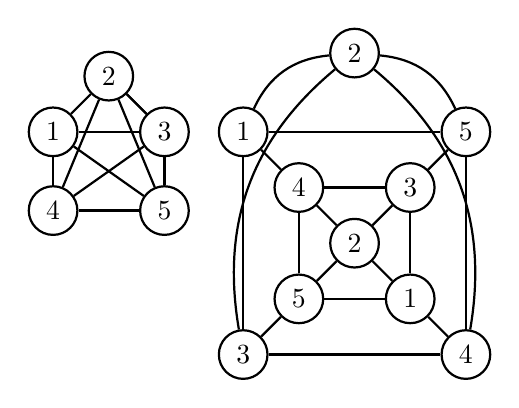
\begin{tikzpicture}[node distance={10mm}, thick, main/.style = {draw, circle}]
			\node[main] (1) {1};
			\node[main] (2) [above right of=1] {2};
			\node[main] (3) [below right of=2] {3};
			\node[main] (4) [below of=1] {4};
			\node[main] (5) [below of=3] {5};
			\draw (1) -- (2);
			\draw (1) -- (3);
			\draw (1) -- (5);
			\draw (2) -- (3);
			\draw (2) -- (3);
			\draw (2) -- (4);
			\draw (2) -- (5);
			\draw (3) -- (4);
			\draw (4) -- (5);
			\draw (1) -- (4);
			\draw (3) -- (5);
			\node[main] (6) [right of=3] {1};
			\node[main] (7) [below right of=6] {4};
			\node[main] (8) [below right of=7] {2};
			\node[main] (9) [below right of=8] {1};
			\node[main] (10) [below right of=9] {4};
			\node[main] (11) [below left of=8] {5};
			\node[main] (12) [below left of=11] {3};
			\node[main] (13) [above right of=8] {3};
			\node[main] (14) [above right of=13] {5};
			\node[main] (15) [above right of=6] [above left of=14] [above of=8] {2};
			\draw (6) -- (7);
			\draw (7) -- (8);
			\draw (8) -- (9);
			\draw (8) -- (11);
			\draw (8) -- (13);
			\draw (9) -- (10);
			\draw (11) -- (12);
			\draw (13) -- (14);
			\draw (7) -- (13);
			\draw (13) -- (9);
			\draw (9) -- (11);
			\draw (11) -- (7);
			\draw (6) -- (14);
			\draw (14) -- (10);
			\draw (10) -- (12);
			\draw (12) -- (6);
			\path
				(6) edge [bend left] (15)
				(14) edge [bend right] (15)
				(10) edge [bend right] (15)
				(12) edge [bend left] (15);
		\end{tikzpicture}
		\caption{Example of $G$ and $G'$ as covers.}
		\label{covers}
	\end{figure}
\end{example}

$$
\begin{array}{c}
	\{G " \exists \text{ planar } G' \text{ cover of } G \} \\
	\Updownarrow \\
	F_{1}, \dots, F_{n} \nleq_{m} G
\end{array}
$$

Contrary we take $\mathcal{G} = \{G : (\forall uv \in V(G) U \neq v, \deg(u) \geq 5, \deg(v) \geq 5) (\exists X \subseteq E(G) : |X| \leq 1) u \text{ and } v \text{ are in different component of } G - X\}$ which is $\leq_{t}$-closed. But take these graphs:

\begin{figure}[!h]\centering
	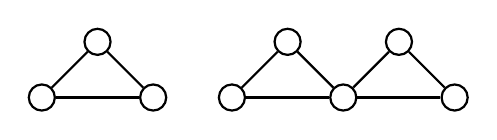
\begin{tikzpicture}[node distance={10mm}, thick, main/.style = {draw, circle}]
		\node[main] (1) {};
		\node[main] (2) [above right of=1] {};
		\node[main] (3) [below right of=2] {};
		\node[main] (4) [right of=3] {};
		\node[main] (5) [above right of=4] {};
		\node[main] (6) [below right of=5] {};
		\node[main] (7) [above right of=6] {};
		\node[main] (8) [below right of=7] {};
		\path
			(1) edge [above] (2)
			(2) edge [above] (3)
			(1) edge [below] (3);
		\path
			(4) edge (5)
			(5) edge (6)
			(6) edge (7)
			(7) edge (8)
			(4) edge (6)
			(6) edge (8);
	\end{tikzpicture}
	\label{endless}
	\caption{Obstructions.}
\end{figure}

Where each one of them is an obstruction. And we could create much more of them.

Now we take a look at some nice properties of graphs if we forbid some graphs as a minors.

$$
\begin{array}{r c l}
	K_{1} \nleq_{m} G & \Leftrightarrow & V(G) = \emptyset \\
	K_{2} \nleq_{m} G & \Leftrightarrow & E(G) = \emptyset \\
	K_{3} \nleq_{m} G & \Leftrightarrow & G \text{ is a forest } \\
	                  &                 & G \text{ is obtained from } K_{1}, K_{2} \text{ by clique sums} \\
	K_{4} \nleq_{m} G & \Leftrightarrow & G \text{ is obtained from } K_{1}, K_{2}, K_{3} \text{ by clique sums} \\
\end{array}
$$

\begin{defn}
	Graph $G$ can be obtained from $G_{1}$ and $G_{2}$ by \textbf{clique-sum} if the inter-\newline section that these graphs have in $G$ form a clique. In other way it is that we bind together two graphs by identifying their vertices and edges in the same size clique. Sometimes we may denote it as $G_{1} \bigoplus G_{2} = G$.
\end{defn}

\begin{observ}
	If $G$ is obtained from $G_{1}$ and $G_{2}$ by a clique-sum then:
	
	$$
	K_{m} \leq_{m} G \Leftrightarrow K_{m} \leq_{m} G_{1} \lor K_{m} \leq_{m} G_{2}
	$$
\end{observ}

\begin{lemma}
	If $K_{k} \leq_{m} G$ and $G$ is the clique-sum of $G_{1}$ and $G_{2}$ then $K_{k} \leq_{m} G_{1} \lor K_{k} \leq_{m} G_{2}$.
\end{lemma}

\begin{lemma}
	If $G$ is not $3$-connected then there exist $G_{1}, G_{2} \lneq_{m} G$ s.t. $G$ is a clique-sum of $G_{1}$ and $G_{2}$.
\end{lemma}

\begin{proof}
	If $G$ is not connected then it is done since it is a clique sum on $K_{0}$. If $G$ is connected, but not $2$-connected then it is a clique-sum on $K_{1}$ since there exist a articulation. If $G$ is $2$-connected then there must be two vertices which splits the graph. And these two vertices form a $K_{2}$ as a minor. That is because we split $G$ to two parts where we leave the major one side and add a edge to these two vertices, which we can do because they need to have a path between them so we contract all the edges alongside the path.
\end{proof}

\begin{defn}
	$\delta(G)$ is a minimum degree of a graph $G$.
\end{defn}

\begin{thm}
	If $G$ is $K_{4}$-minor-free then $G$ is obtained from $K_{\leq 3}$'s by clique-sums.
\end{thm}

\begin{proof}
	By induction on $|V(G)|$.
	
	\begin{enumerate}[(a)]
		\item If $G$ is not 3-connected. $G$ is a clique-sum of $G_{1},G_{2} \lneq_{m} G$. Since $K_{4} \nleq_{m} G_{1}$ and $K_{4} \nleq_{m} G_{2}$ we use induction hypothesis and we are done.
		\item If $G$ is 3-connected. If $|V(G)| \leq 3$, then $G = K_{\leq 3}$, wlog $|V(G)| \geq 4$. $\delta(G) > 1 \Rightarrow G$ contains a cycle. Let $C$ be a shortest cycle in $G$. $C$ is induced in $G$ 3-connected $\Rightarrow G \neq C$ so $\exists v \in V(G) \setminus V(C)$. By Merger's theorem there exists three paths from $v$ to $C$ intersecting only in $v$. That gives us $K_{4}$ as a minor of the graph. Which is contradiction.
	\end{enumerate}
\end{proof}

$$
\begin{array}{r c l}
	K_{5} \nleq_{m} G & \Leftrightarrow & G \text{ is obtained from planar graphs and } W_{8}  \text{ by clique sums} \\
\end{array}
$$

\begin{figure}[!h]\centering
	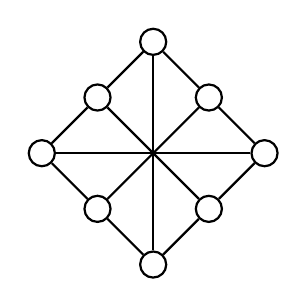
\begin{tikzpicture}[node distance={10mm}, thick, main/.style = {draw, circle}]
		\node[main] (1) {};
		\node[main] (2) [above right of=1] {};
		\node[main] (3) [below right of=2] {};
		\node[main] (4) [below left of=1] {};
		\node[main] (5) [below right of=3] {};
		\node[main] (6) [below left of=5] {};
		\node[main] (7) [below right of=4] {};
		\node[main] (8) [below right of=7] {};
		\draw (1) -- (2);
		\draw (4) -- (1);
		\draw (4) -- (7);
		\draw (7) -- (8);
		\draw (8) -- (6);
		\draw (6) -- (5);
		\draw (3) -- (5);
		\draw (2) -- (3);
		\draw (2) -- (8);
		\draw (1) -- (6);
		\draw (4) -- (5);
		\draw (7) -- (3);
	\end{tikzpicture}
	\caption{$W_{8}$ graph.}
	\label{w8}
\end{figure}

\begin{observ}
	If $G$ is a clique-sum of $G_{1}$ and $G_{2}$ then
	
	$$
	\chi(G) \leq \max (\chi(G_{1}), \chi(G_{2}))
	$$
\end{observ}

\begin{proof}
	We just need to match the coloring of the cliques. Other than that we don't have any problem.
\end{proof}

\section{Hadwiger's conjecture}

$K_{t}$-minor-free graphs are $(t-1)$ colorable.

$$
\begin{array}{c c c}
	K_{1} \nleq_{m} G & \chi \leq 1 & \delta \leq 0 \\
	K_{2} \nleq_{m} G & \chi \leq 2 & \delta \leq 1 \\
	K_{3} \nleq_{m} G & \chi \leq 3 & \delta \leq 2 \\
	K_{4} \nleq_{m} G & \chi \leq 4 & \delta \leq 5 \\
	K_{5} \nleq_{m} G & \chi \leq 5 & \\
\end{array}
$$

\begin{thm}
	$\exists f$ every $K_{t}$-minor-free graph $G$ has $\delta(G) \leq f(t)$.
\end{thm}

The function is somewhere near $f(t) = (1,6\dots + O(1)) t \sqrt{\log t}$. But we won't show this result. Instead we will show $f(t) = O(t^{2})$. Before we continue it is better to remind ourselves \textbf{chordal graph} and \textbf{elimination ordering} (known as PES).

\begin{defn}[Chordal decomposition of $G$]
	$V(G) = \mathcal{P}_{1} \dot{\cup} \mathcal{P}_{2} \dot{\cup} \dots \dot{\cup} \mathcal{P}_{n} \dot{\cup}$ and
	
	\begin{enumerate}
		\item $(\forall i) G[\mathcal{P}_{i}]$ is connected.
		\item "$\mathcal{P}_{i}$'s form elimination ordering" Precisely: $(\forall i \in [n])(forall j_{1},j_{2} < i)$ if $G$ has an edge between $\mathcal{P}_{i}$ and $\mathcal{P}_{j_{1}}$ and also between $\mathcal{P}_{i}$ and $\mathcal{P}_{j_{2}}$ then it also has an edge between $\mathcal{P}_{j_{1}}$ and $\mathcal{P}_{j_{2}}$.
	\end{enumerate}
\end{defn}

\begin{defn}
	Chordal partition is \textbf{geodesic} if $(\forall i) (\exists v_{i} \in \mathcal{P}_{i})$ s.t. if $v_{1}, \dots, v_{t} < i$ are the indices s.t. $G$ has an edge between $\mathcal{P}_{i}$ and $\mathcal{P}_{j_{1}}, \mathcal{P}_{j_{2}}, \dots, \mathcal{P}_{j_{t}}$ then $v_{1}, \dots, v_{t} \in \mathcal{P}_{i}$ s.t. $v_{i}$ has a neighbor in $\mathcal{P}_{j_{1}}, \mathcal{P}_{j_{2}}, \dots, \mathcal{P}_{j_{t}}$ and $G - \bigcup_{j < i} \mathcal{P}_{j}$ contains shortest paths from $v_{i}$ to $v_{1}, \dots, v_{t}$ which cover all vertices in $\mathcal{P}_{i}$.
\end{defn}

% TODO perhaps add an image

\begin{thm}
	Every graph has a geodesic chordal partition.
\end{thm}

Before we show us a proof we will take a look at a simple application. If $G$ is $K_{k}$-minor-free last part has neighbours in $t \leq k-2$ parts (otherwise it will have $K_{k}$ as a minor). Then we may take a look at a $\deg(v) \leq (k-2) + (k-2)(k-2)3 \leq 3k^{2}$. Thus getting the upper bound $\delta(G) \leq 3k^{2}$.

\begin{defn}
	Part is called \textbf{terminal} if there is no edge from any vertex in that part going to some vertex in one of the parts on the right.
\end{defn}

\begin{proof}
	Let $\mathcal{P}$ be a chordal decomposition of $G$ into parts satisfying both properties of definition of chordal decomposition (i) abd (ii) and geodesity (iii) for all non-terminal parts.
	
	This can be easily done by creating parts based on the components of connectivity. For them all properties hold, since they are all connected and "chordal" property is also satisfied since there are no edges. Also all of them are terminal (iii) doesn't have to be satisfied.
	
	Now we proof by that by choosing $\mathcal{P}$ with largest number of parts. Lets say that there is a part that does not satisfy (iii). This means that it is terminal part. Lets take vertex from the part and find the shortest paths to the vertices that are connected to some of the parts to the left. Now we put vertices to separate components and these components will make a new parts. We will also remove all these vertices from the origin part. Note that all properties are satisfied. (i) is trivial. (ii) If there are any vertices from the new parts to other parts then they are to the ones which are already connected to the origin part, which satisfied (ii) before so it is fine. Also (iii) is satisfied.
	
	The thing is that we created $\mathcal{P}$ with larger number of parts which is contradiction.
\end{proof}

\begin{observ}
	$H \leq_{t} G \Rightarrow H \leq_{m} G$
\end{observ}

\begin{observ}
	$\Delta (H) \leq 3 : H \leq_{m} G \Rightarrow H \leq_{t} G$
\end{observ}

Lets remind ourselves a table and add some new thinks.

$$
\begin{array}{ r c l}
	K_{1} \nleq_{t} G \Leftrightarrow K_{1} \nleq_{m} G & \Leftrightarrow & V(G) = \emptyset \\
	K_{2} \nleq_{t} G \Leftrightarrow K_{2} \nleq_{m} G & \Leftrightarrow & E(G) = \emptyset \\
	K_{3} \nleq_{t} G \Leftrightarrow K_{3} \nleq_{m} G & \Leftrightarrow & G \text{ is a forest } \\
	&                 & G \text{ is obtained from } K_{1}, K_{2} \text{ by clique sums} \\
	K_{4} \nleq_{t} G \Leftrightarrow K_{4} \nleq_{m} G & \Leftrightarrow & G \text{ is obtained from } K_{1}, K_{2}, K_{3} \text{ by clique sums} \\
	K_{5} \nleq_{t} G \nLeftrightarrow K_{5} \nleq_{m} G & \Leftrightarrow & G \text{ is obtained from planar graphs and } W_{8}  \text{ by clique sums} \\
\end{array}
$$

Well technically $K_{5} \nleq_{t} G \Rightarrow K_{5} \nleq_{m} G$ but the other way around is what doesn't work $K_{5} \nleq_{m} G \nRightarrow K_{5} \nleq_{t} G$. For that we can see an example \ref{minor-not-top}. We may see that $\mathcal{G} = \{G : G \text{ has } \leq 4 \text{ vertices of degree } \geq 4\}$ these graphs are so that $K_{5} \nleq_{t} G$.

\begin{figure}[!ht]\centering
	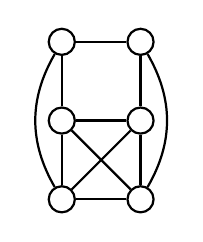
\begin{tikzpicture}[node distance={10mm}, thick, main/.style = {draw, circle}]
		\node[main] (1) {};
		\node[main] (2) [right of=1] {};
		\node[main] (3) [below of=1] {};
		\node[main] (4) [below of=2] {};
		\node[main] (5) [below of=3] {};
		\node[main] (6) [below of=4] {};
		\draw (1) -- (2);
		\draw (1) -- (3);
		\draw (4) -- (2);
		\draw (3) -- (4);
		\draw (5) -- (4);
		\draw (6) -- (4);
		\draw (6) -- (5);
		\draw (3) -- (5);
		\draw (3) -- (6);
		\path
			(1) edge [bend right] (5)
			(2) edge [bend left] (6);
	\end{tikzpicture}
	\caption{A counter example.}
	\label{minor-not-top}
\end{figure}

\section{Hájos conjecture}

If we remember Headwiger's conjecture then Hájos conjecture is the same only with topological minors. Thus it is that $K_{t} \leq_{t} G \Rightarrow \chi(G) \leq t-1$. This is actually true for $t < 4$ but it is false for $t \geq 7$ and $5,6$ are open questions.

\begin{thm}
	$\exists f_{m}(k) = O(k \sqrt{\log k})$ Every $K_{k}$-minor-free graph $G$ satisfies $\delta(k) \leq f_{m}(k)$.
\end{thm}

We won't proof this, but we will proof something similiar, that is for topological minors.

\begin{thm}
	$\exists f_{t}(k) = O(k^{2})$ Every $G$ s.t. $K_{k} \lneq_{t} G$ satisfies $\delta(G) \leq f_{t}(k)$.
\end{thm}

The corollary to this is that $\chi)G_ \leq f_{t}(k) +1$. We will proof this theorem, but to do that we need to do some steps beforehand.

Firstly imagine that the enemy gives you a graph and you need to prove that. But the enemy is kind enough to give you a graph $H$ with connectivity $>> k^2$. We could apply Merger's theorem. Though this will only give certain number of vertex disjoint paths from one vertex to another. We would more likely have this many paths between more pairs of sources and targets.

\begin{defn}
	Graph $G$ is \textbf{$k$-linked} if $|V(G)| \geq 2k$ and $\forall s_{1}, s_{2}, \dots, s_{k}, t_{1}, t_{2}, t_{k}$ distinct vertices of $G$. $G$ contains pairwise vertex-disjoint paths $P_{1}, P_{2}, \dots, P_{k}$. When $P_{i}$ has ends $s_{i}$ and $t_{i}$.
\end{defn}

We may see that there exist a graph that is 2-connected and yet not 2-linked. You may see this on the picture \ref{2-linked-2}. Also not even 3-connected graph has to be 2-linked. Which is also on the picture \ref{2-linked-3} (though we can change the vertex inside for any planar graph). We could continue and end up with that not even 5-connectivity forces 2-linked.

\begin{figure}[!ht]\centering
	\begin{subfigure}[b]{0.4\textwidth}\centering
		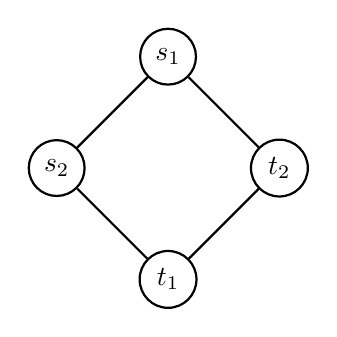
\begin{tikzpicture}[node distance={20mm}, thick, main/.style = {draw, circle}]
			\node[main] (1) {$s_{1}$};
			\node[main] (2) [below left of=1] {$s_{2}$};
			\node[main] (3) [below right of=1] {$t_{2}$};
			\node[main] (4) [below right of=2] {$t_{1}$};
			\draw (1) -- (2);
			\draw (2) -- (4);
			\draw (3) -- (4);
			\draw (3) -- (1);
		\end{tikzpicture}
		\caption{2-connectivity}
		\label{2-linked-2}
	\end{subfigure}
	\begin{subfigure}[b]{0.4\textwidth}\centering
		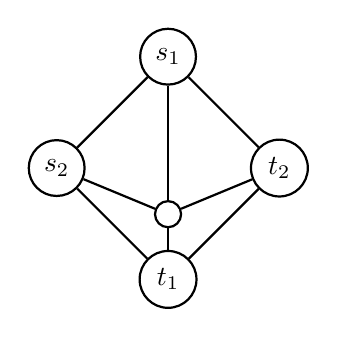
\begin{tikzpicture}[node distance={20mm}, thick, main/.style = {draw, circle}]
			\node[main] (1) {$s_{1}$};
			\node[main] (2) [below left of=1] {$s_{2}$};
			\node[main] (3) [below right of=1] {$t_{2}$};
			\node[main] (4) [below right of=2] {$t_{1}$};
			\node[main] (5) [below of=1] {};
			\draw (1) -- (2);
			\draw (2) -- (4);
			\draw (3) -- (4);
			\draw (3) -- (1);
			\draw (1) -- (5);
			\draw (2) -- (5);
			\draw (3) -- (5);
			\draw (4) -- (5);
		\end{tikzpicture}
		\caption{3-connectivity}
		\label{2-linked-3}
	\end{subfigure}
	\caption{A counter example to 2-linked graphs.}
	\label{2-linked}
\end{figure}

\begin{observ}
	Every $k$-linked graph is $(2k-1)$ connected.
\end{observ}

\begin{proof}
	That is simply because we put all the $s_{i}, t_{i}$ for $i \in [k-1]$ to the edge cut and then choose $s_{k}$ in the left part and $t_{k}$ in the right part then we can see that it is indeed $(2k-1)$-connected.
\end{proof}

\begin{thm}\label{2-linked-thm}
	If $G$ is $2k$-connected, $K_{4k} \leq_{m} G$ then $G$ is $k$-linked.
\end{thm}

We won't prove this directly. Instead we will later on introduce another theorem that is actually pretty much the same and prove that.

\begin{cor}
	If $G$ is $\max(2k, f_{m}(4k)+1)$-connected then $G$ is $K$-linked.
\end{cor}

\begin{proof}
	We use the theorem to get that $\delta > f_{m}(4k)$ thus $K_{4k} \leq_{m} G$.
\end{proof}

Also we can say $\exists f_{l}(k) = O(k \sqrt{\log k})$. If $G$ is $f_{l}(k)$-connected then $G$ is $k$-linked.

\begin{cor}
	If $G$ is $f_{l}\left( \frac{k (k-1)}{2}\right)$-connected then $K_{k} \leq_{t} G$.
\end{cor}

\begin{proof}
	To see this we choose $k$ vertices and for every one of them $k-1$ neighbors. Then we give $s_{i}$ and $t_{i}$ to every single one of these vertex so that every neighborhood has pair with all others. Then we find such paths between them.
\end{proof}

\begin{lemma}
	If $\bar{d}(G) \geq 4d$ then $G$ contains a $(d+1)$-connected subgraph $H$ of minimum degree $2d+1$.
\end{lemma}

\begin{proof}
	Let $H$ be a minimal subgraph of $G$ s.t. $|V(H)| \geq 2d$ and $|E(H)| > 2d (|V(H)| - d)$. We may see that $|V(H)| > 2d$ that is if it has $2d$ vertices then
	
	$$
	\frac{2d^{2} - d}{2} = \binom{2d}{2} > |E(H)| > 2d^{2}
	$$
	
	which is a contradiction.
	
	Then we also have that $\delta (H) \geq 2d+1$. If we have $\delta(H) \leq 2d$ we may remove the certain vertex. But we need to show that given properties still hold. We will split the graph to two parts $|A|, |B| \geq 2d+2 > 2d$. Then
	
	$$
	\begin{array}{r l}
		|E(G)| & \leq |E(A)| + |E(B)| \\
		(1) & \leq 2d(|V(A)| - d) + 2d(|V(A)| - d) \\
		& = 2d(|V(A)| + |V(B)| - 2d) \\
		& = 2d(|V(H)| - |V(A \cap B)| - 2d) \\
		|E(G)| & > 2d(|V(H)| - d)
	\end{array}
	$$
	
	Where $(1)$ is due to the minimality of $H$. The thing is with the last two lines we get that $|A \cap B| > d$.
\end{proof}

\begin{proof}
	This actually is enough for the theorem to be proven since the enemy doesn't have to be kind anymore.
\end{proof}

\begin{defn}
	A \textbf{model} of $K_{m}$ in $G$ is $M_{1}, M_{2}, \dots, M_{m} \subseteq V(G)$ pairwise distinct and $\forall i : G[M_{i}]$ is connected and $(\forall i \neq j) \exists uv \in E(G): u \in M_{i}, v\in M_{j}$.
\end{defn}

We may take a look at an example of model of $K_{4}$ which is in picture \ref{k4-model}.

\begin{figure}[!ht]\centering
	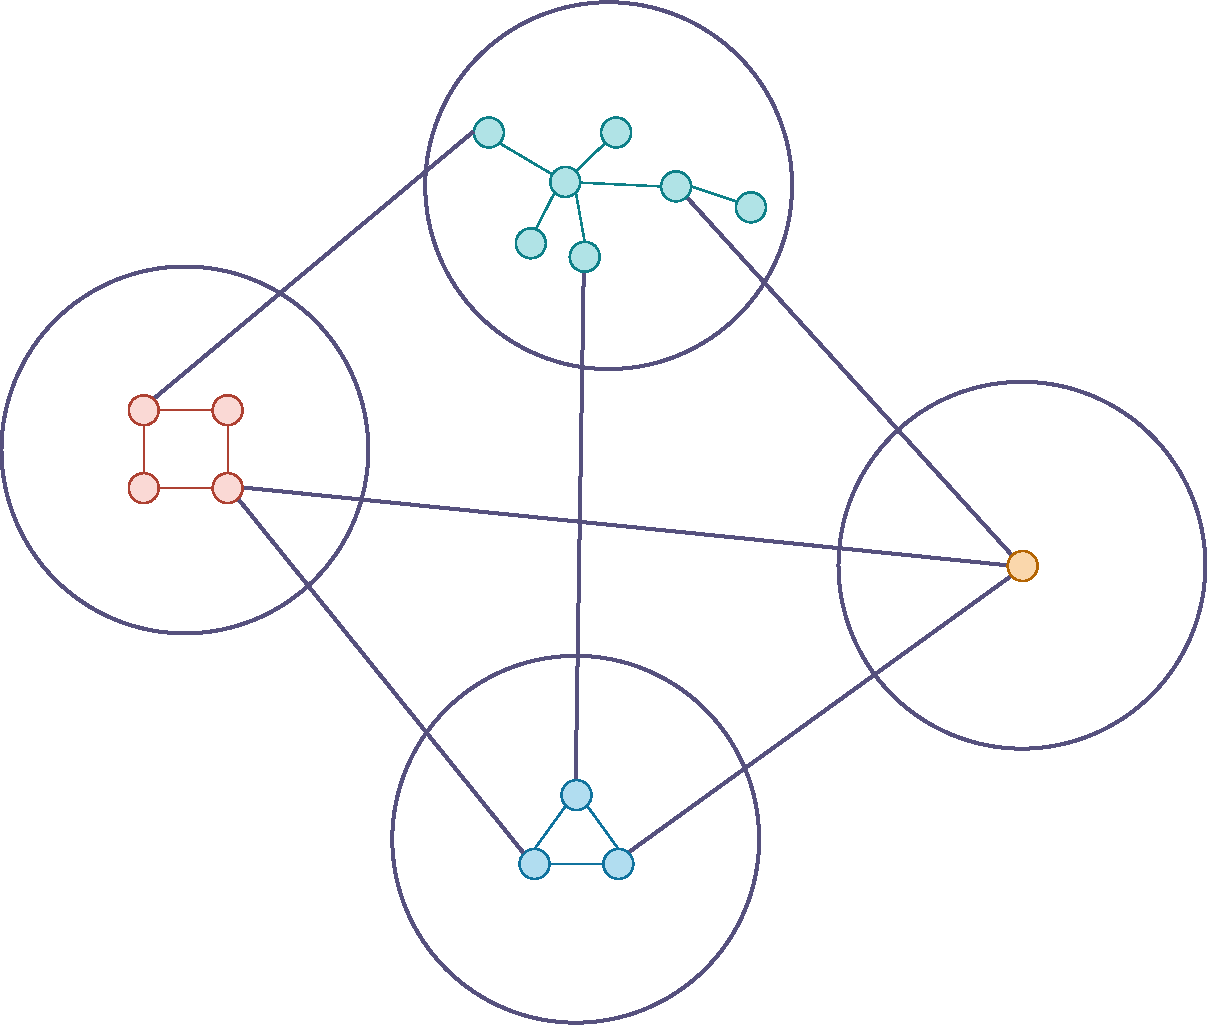
\includegraphics[width=0.5\textwidth]{res/km-model.pdf}
	\caption{Example of $K_{4}$ model.}
	\label{k4-model}
\end{figure}

\begin{observ}
	$K_{m} \leq_{m} G \Leftrightarrow \text{there is a mode of } K_{m} \text{ in } G$.
\end{observ}

\begin{defn}
	\textbf{Separation} in $G$ is $(A,B)$ where $A,B \subseteq V(G), A \cup B = V(G)$, no edge between $A \setminus B$ and $B \setminus A$.
\end{defn}

On picture \ref{separation} we may see an example of $(A,B)$-separation.

\begin{figure}[!ht]\centering
	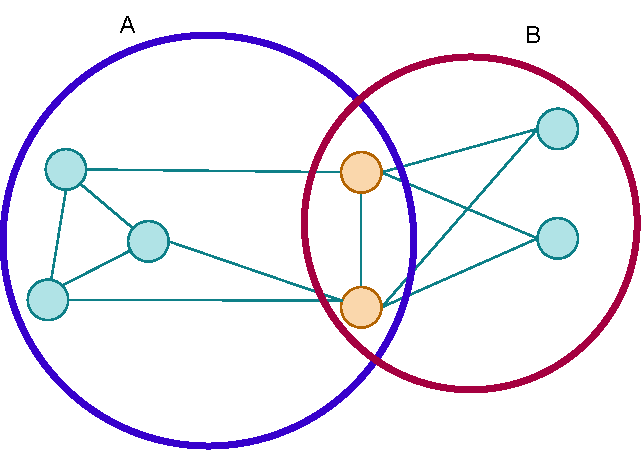
\includegraphics[width=0.3\textwidth]{res/separation.pdf}
	\caption{Example of separation.}
	\label{separation}
\end{figure}

\begin{defn}
	The \textbf{order} of the separation is $|A \cap B|$.
\end{defn}

\begin{defn}
	$S$ is \textbf{well-linked} to a model $M_{1}, M_{2}, \dots, M_{m}$ if every separation $(A,B)$ with $S \subseteq A_{i}$ $(\exists i) M_{i} \subseteq B \setminus A$ has order $\geq |S|$.
\end{defn}

\begin{thm}
	$\forall G_{i}, S = \{s_{1}, s_{2}, \dots, s_{k}, t_{1}, t_{2}, \dots, t_{k}\} \subseteq V(G)$ and $M_{1}, \dots, M_{4k}$ mdel of $K_{4m}$ in $G$. If $S$  is well-linked to $M_{1}, M_{2}, \dots, M_{4k}$ then $G$ contains distinct paths from $s_{i}$ to $t_{i}$ for all $i \in [k]$.
\end{thm}

We can see that this is somewhat refolmulation of theorem before (\ref{2-linked-thm}). Thus if we prove this we will also prove the previous theorem. But we will introduce another similiar theorem which will imply this theorem.

\begin{defn}
	$G, S\ subseteq V(G)$ and $M_{1}, M_{2}, \dots, M_{m} \subseteq V(G)$ pairwise distinct is an \textbf{$S$-relaxed model} of $K_{m}$ in $G$ if
	
	\begin{enumerate}
		\item $(\forall i) G[M_{i}]$ is connected \underline{or} every componnet of $G[M_{i}]$ intersects $S$.
		\item $(\forall i \neq j) \exists uv \in E(G)$ s.t. $u \in M_{i}, v \in M_{j}$ \underline{or} $M_{i} \cap S \neq \emptyset \neq M_{j} \cap S$.
	\end{enumerate}
\end{defn}

\begin{thm}[\textcolor{blue}{Slightly changed}]
	$\forall G_{i}, S = \{s_{1}, s_{2}, \dots, s_{k}, t_{1}, t_{2}, \dots, t_{k}\} \subseteq V(G)$ and $M_{1}, \dots, M_{4k}$ \textcolor{blue}{$S$-relaxed mdel} of $K_{4m}$ in $G$. If $S$  is well-linked to $M_{1}, M_{2}, \dots, M_{4k}$ then $G$ contains distinct paths from $s_{i}$ to $t_{i}$ for all $i \in [k]$.
\end{thm}

\begin{proof}
	We will prove this theorem by induction on $|V(G)|$. We will separate it to some distinct cases.
	
	\begin{enumerate}[(1)]
		\item Suppose there exisits a separation $(A,B)$ of order $2k$ (which is $= |S|$) s.t. $S \subsetneq A$ and $(\exists i) M_{i} \subseteq B \setminus A$. Then by Menger's theorem there exists $2k$ disjoint paths from $S$ to $A \cap B$ (since $S$ is well-linked to $M_{1}, \dots, M_{4k}$).\textit{ We want: $G[B]$ disjoint paths from $s_{i}'$ to $t_{i}'$ for all $i \in [k]$, where $s_{i}'$ and $t_{i}'$ are the ends from the paths labeled same as the beginings.} We apply induction hypothesis on $G[B]$ $S' = \{s_{i}', t_{i}' | \forall i \in [k]\}$ $M_{1} \cap B, M_{2} \cap B, \dots, M_{4k} \cap B$.
		
		First we need to prove that the properties still holds. Such as that it is still $S'$-relaxed and $S'$ is well-linked. Consider $M_{i} \cap S = \emptyset$ so $\forall j \neq i$ there is at least one vertex in $B$. Then $M_{1} \cap B$ components do not intersect $S'$ so it didn't intersect $S$. Therefore it had to be connected and thus still is. That is the first property and the second is \textit{left out as exercise}. So $S'$ is relaxed model.
		
		We now take a look at if $S'$ wouldn't be well-linked. Then there would be a separation with order $< 2k$. But this separation would be present even before so it cannot be there.
		
		Now WLOG: Every separation $(A,B)$ s.t. $S \subsetneq A, (\exists i) M_{i} \subseteq B \setminus A$ has order $> 2k$.
		
		\item Suppose $\exists v \in V(G) \setminus (S \cup \bigcup_{i}^{4k} M_{i})$ apply I.H. on $G -v$. We need to show that it is well-linked. Suppose we have a separation with order $<2k$. We put $v$ in the intersection of the separation ("cut") and get a separation of $G$ with order $\leq 2k$. That can't happen since we assumed the orrder is $>2k$.
		
		\item Suppose $(\exists i) \exists uv \in E(G[M_{i}])$ s.t. $v \notin S$. Aplly I.H> to $G / uv$ (contract the edge $uv$). We may see that $S$ is relaxed model and well-linked with the similiar arguments as in the point before.
	\end{enumerate}
	
	With this induction we end up with $S \subseteq V(G)$ and $M_{1}, M_{2}, \dots, M_{4k}$. We know $(\forall i) M_{i} \cap S = \emptyset \Rightarrow |M_{i}| =1$ \underline{or} $M_{i} \subseteq S$. Also all single $M_{i}$ forms a clique. We would like to find if there exist a mathcing between $S$ and $V(G) \setminus S$ covering $S$. For that we may recall Hall's theorem and thus we need $\forall X \subseteq S: |N(X)| \geq |X|$ where $N(X)$ are the neighbours of $X$. Lets take a look at one $M_{k} = X$ and its $N(X)$. There are not necessarily edges to $M_{1}, \dots, M_{g}$. Lets put $A = S \cup N(X)$ and $B = \text{ clique on } M_{i}\text{s} \cup (S \setminus X)$. By that we get that $X = A \setminus B$ and $V(G) \setminus (S \cup N(X)) = B \setminus A$. So $(S \setminus X) \cup N(X) = A \cap B$ which can't be smaller than $2k$. So $|S \setminus X| + |N(X)| \geq 2k$ where $S \setminus X| = |S| - |X|$ and $|S| = 2k$ this means that $|N(x)| \geq |X|$.
	
	Therefore we find the matching between $S$ and clique. Thus we take for each $i$ the edge in matching from $s_{i}$ to $s_{i}'$, then path from clique from $s_{i}'$ to $t_{i}'$ and next from matching $t_{i}'$ to $t_{i}$.
\end{proof}
	\chapter{Tree decomposition}

Firstly we may recall that: $K_{5} \nleq_{m} G$ iff $G$ is obtained from planar graphs and $W_{8}$'s by clique-sums. When we draw the graphs expanding by the clique sums we may notice a somewhat tree structure that they generate. Now we will define it and see it properly.

\section{Basics}

\begin{defn}
	A \textbf{tree decomposition} $(T, \beta)$ of graph $G$ is when $T$ is a tree and $\beta: V(T) \to 2^{V(G)}$ (\textit{called bags}) such that
	
	\begin{enumerate}[(1)]
		\item $(\forall uv \in E(G)) (\exists x \in V(T)): u,v \in \beta(x)$ or by words every edge is contained in a bag.
		\item $\forall v \in V(G)$ the set $\{x \in V(T) : v \in \beta(x)\}$ induces a non-empty connected subtree of $T$.
	\end{enumerate}
\end{defn}

\begin{lemma}
	If $(T, \beta)$ is a tree decomposition of $G$, $K \subseteq V(G)$ is a clique in $G$ then $(\exists x \in V(T)) : K \subseteq \beta(x)$.
\end{lemma}

\begin{proof}
	For contradiction suppose it is not true. Thus $(\forall x \in V(T)) (\exists v_{x} \in K) : v_{x} \notin \beta(x)$. We define "arrows" for each vertex which points to the set $\{y : v_{x} \notin \beta(x)\}$. Thus there is $|V(T)|$ of "arrows" but because it is a tree there is $|E(T)| = |V(T)| - 1 < |V(T)|$. So at least one edge must have two "arrows". Therefore there is no $y \in V(T)$ with $v_{x}, v_{x'} \in \beta(x)$ so $K$ clique implies that $v_{x}$ and $v_{x'}$ are adjacent. This is contradiction with (1) from definition.
\end{proof}

\begin{defn}
	$(T, \beta)$ is tree decomposition of $G$ and let $x \in V(T)$ then the \textbf{torso} of $x$. is $G[\beta(x)] + $ cliques on $\beta(x) \cap \beta(y)$ for every $xy \in E(T)$.
\end{defn}

This definition may not be clear to everybody so lets take a look at an example. On picture \ref{example-torso} we may see the original graph \ref{g-torso} and on picture \ref{t-torso} we may see the tree decomposition. Now we set $x$ to be \texttt{BGE}. Now for the torso itself we create a three vertices \texttt{B}, \texttt{G} and \texttt{E} where there is no induced edge. Then for the neighbors \texttt{ABG} we add a edge between \texttt{B} and \texttt{G}. For \texttt{BED} we add an edge between \texttt{B} and \texttt{E} and lastly for \texttt{EGF} we add \texttt{E}--\texttt{G} edge. And finally we get what is drawn on picture \ref{torso}.

\begin{figure}[!ht]\centering
	\begin{subfigure}{0.4\textwidth}\centering
		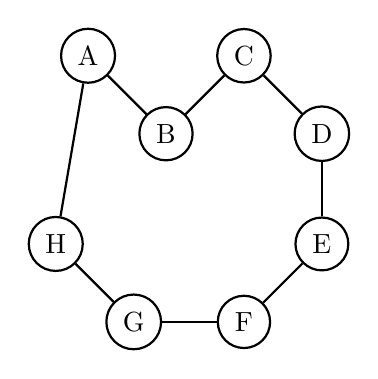
\begin{tikzpicture}[node distance={14mm}, thick, main/.style = {draw, circle}]
			\node[main] (1) {A};
			\node[main] (2) [below right of=1] {B};
			\node[main] (3) [above right of=2] {C};
			\node[main] (4) [below right of=3] {D};
			\node[main] (5) [below of=4] {E};
			\node[main] (6) [below left of=5] {F};
			\node[main] (7) [left of=6] {G};
			\node[main] (8) [above left of=7] {H};
			\path
				(1) edge (2)
				(2) edge (3)
				(3) edge (4)
				(4) edge (5)
				(5) edge (6)
				(6) edge (7)
				(7) edge (8)
				(8) edge (1);
		\end{tikzpicture}
		\caption{Original graph $G$.}
		\label{g-torso}
	\end{subfigure}
	\begin{subfigure}{0.4\textwidth}\centering
		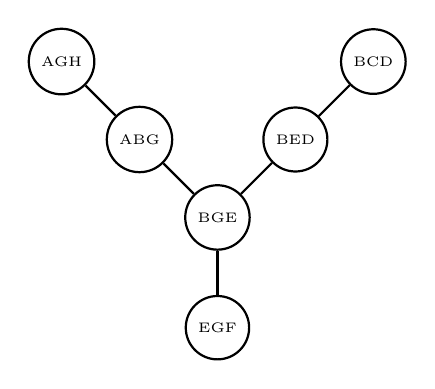
\begin{tikzpicture}[node distance={14mm}, thick, main/.style = {draw, circle}]
			\node[main] (1) {\tiny{AGH}};
			\node[main] (2) [below right of=1] {{\tiny ABG}};
			\node[main] (3) [below right of=2] {{\tiny BGE}};
			\node[main] (4) [above right of=3] {{\tiny BED}};
			\node[main] (5) [above right of=4] {{\tiny BCD}};
			\node[main] (6) [below of=3] {{\tiny EGF}};
			\path
			(1) edge (2)
			(2) edge (3)
			(3) edge (4)
			(4) edge (5)
			(3) edge (6);
		\end{tikzpicture}
		\caption{Tree decomposition of $G$.}
		\label{t-torso}
	\end{subfigure}
	\caption{An example of \textbf{torso.}}
	\label{example-torso}
\end{figure}

\begin{figure}[!ht]\centering
	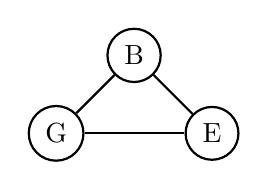
\begin{tikzpicture}[node distance={14mm}, thick, main/.style = {draw, circle}]
		\node[main] (1) {B};
		\node[main] (2) [below right of=1] {E};
		\node[main] (3) [below left of=1] {G};
		\path
		(1) edge (2)
		(2) edge (3)
		(3) edge (1);
	\end{tikzpicture}
	\caption{Actual \textbf{torso} of $x$.}
	\label{torso}
\end{figure}

\begin{lemma}
	Let $\mathcal{G}$ be a class of graphs. $G$ is obtained by clique-sums from graphs belonging to $\mathcal{G}$ iff $G$ has a tree decomposition whose torsos belongs to $\mathcal{G}$.
\end{lemma}

\begin{proof}
	Firstly the "$\Leftarrow$" is easy since when taken the tree decomposition torso we may see that it is somewhat the same as clique-sum of the graphs.
	
	Next we have "$\Rightarrow$" for them we will prove it by induction on the number of terms.
	
	\begin{enumerate}[(i)]
		\item When we have one term than the whole $G \in \mathcal{G}$ and we take a tree decomposition with only one vertex having all vertices from $G$.
		\item Now we have $G = G_{1} \bigoplus_{K} G_{2}$ thus there by induction hypothesis we have $(T_{1}, \beta_{1})$ and $(T_{2}, \beta_{2})$ tree decompositions of their respected graphs $G_{1}$ and $G_{2}$. By lemma there exists a bag with clique $K$ in both $T_{1}$ and $T_{2}$. So we create $T$ by adding edge between those bags in $T_{1}$ and $T_{2}$. So $(T, \beta = \beta_{1} \cup \beta_{2})$ will be the tree decomposition. While it may seem easy it is necessary to show that all properties holds. Every edge is contained in at least one bag since we did not added no edge. Secondly all $x$ induces a non-empty connected subtree.
		
		Also we have to take a look at the torsos we are getting from this tree decomposition. For those bags not having new edge it is still the same as before and for bag $\beta(x)$ which $K \subseteq \beta(x)$ we see that its only intersection is $K$ so it won't change any torso because it is a clique.
	\end{enumerate}
\end{proof}

\section{Tree width}

So we introduced basic tree decomposition but now we take a deeper look at some special cases of them.

\begin{defn}
	\textbf{Width} of $(T, \beta)$ is $\max_{x \in V(T)} (|\beta(x)|) -1$.
\end{defn}

\begin{defn}
	We denote $\text{tw}(G) = \min$ width of $(T, \beta)$ for all $(T, \beta)$ tree decompositions of $G$. It is called the \textbf{treewidth}.
\end{defn}

We may recall and extend that for $k \leq 4$: $K_{k} \nleq_{m} G$ iff $G$ is obtained by clique-sum from graphs with $\leq k-1$ vertices iff $G$ having tree decomposition $(T, \beta)$ such that $(\forall x \in V(T)) : |\beta(x)| \leq k-1$ which means that $\text{width}(T, \beta) \leq k - 2$ iff $\text{tw}(G) \leq k - 2$.

We would now need $\{G : \text{tw}(G) \leq k\}$ is minor-closed.

\begin{observ}
	$H \leq_{m} G \Rightarrow \text{tw}(H) \leq \text{tw}(G)$
\end{observ}

\begin{proof}
	We may see all possible operations. First deletion of vertex may only decrease the value. Second the deletion of edge may also only decrease the value. Lastly for contracting an edge $uv$ we overwrite all these vertices to $w$ and change the edges. This is easily seen that it will only decrease the value or it will stay the same.
\end{proof}

From that we get that $\exists \mathcal{F}_{k}$ $\text{tw}(G) \leq k$ iff $(\forall F \in \mathcal{F}_{k}) F \nleq_{m} G$. Also for some simple values we know $\mathcal{F}_{1} = \{K_{3}\}$ also $\mathcal{F}_{2} = \{K_{4}\}$ and for $\mathcal{F}_{3} = \{K_{5, \dots }\}$ where it is known but not that important.

\section{Bramble}

\begin{defn}
	Bramble $\mathcal{B} \subseteq 2^{V(G)}$ such that
	
	\begin{enumerate}[(1)]
		\item $(\forall B \in \mathcal{B}) B \neq \emptyset$ and $G[B]$ is connected.
		\item $(\forall B_{1}, B_{2} \in \mathcal{B})$ $G[B_{1} \cup B_{2}]$ is connected.
	\end{enumerate}
\end{defn}

As previously we will take a look at an example of a bramble so that a reader gets a better grasp on this definition. On the picture \ref{rumble-example} we may see a graph $G$ where there is Bramble $\mathcal{B} = \{B_{1}, B_{2}, B_{3}, B_{4}\}$.

\begin{figure}[!ht]\centering
	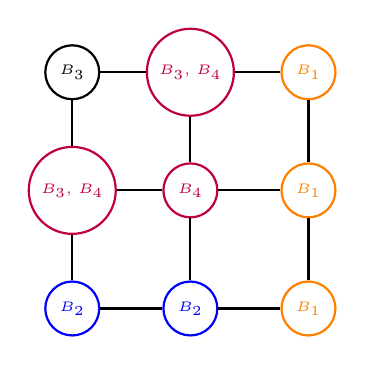
\begin{tikzpicture}[node distance={15mm}, thick, main/.style = {draw, circle}]
		\node[main] (1) [color=black] {{\tiny $B_{3}$}};
		\node[main] (2) [right of=1] [color=purple] {{\tiny $B_{3}$, $B_{4}$}};
		\node[main] (3) [right of=2] [color=orange] {{\tiny $B_{1}$}};
		\node[main] (4) [below of=1] [color=purple] {{\tiny $B_{3}$, $B_{4}$}};
		\node[main] (5) [right of=4] [color=purple] {{\tiny $B_{4}$}};
		\node[main] (6) [right of=5] [color=orange] {{\tiny $B_{1}$}};
		\node[main] (7) [below of=4] [color=blue] {{\tiny $B_{2}$}};
		\node[main] (8) [right of=7] [color=blue] {{\tiny $B_{2}$}};
		\node[main] (9) [right of=8] [color=orange] {{\tiny $B_{1}$}};
		\path
			(1) edge (2) (2) edge (5)
			(2) edge (3) (3) edge (6)
			(1) edge (4) (5) edge (8)
			(4) edge (7) (6) edge (9)
			(4) edge (5) (5) edge (6)
			(7) edge (8) (8) edge (9);
	\end{tikzpicture}
	\caption{Bramble of a graph $G$.}
	\label{rumble-example}
\end{figure}

\begin{defn}
	Set $X$ \textbf{hits} the Bramble $\mathcal{B}$ if $(\forall B \in \mathcal{B}) B \cap X \neq \emptyset$.
\end{defn}

For the previous example a hit could be all these vertices highlighted on the picture \ref{hit}.

\begin{figure}[!ht]\centering
	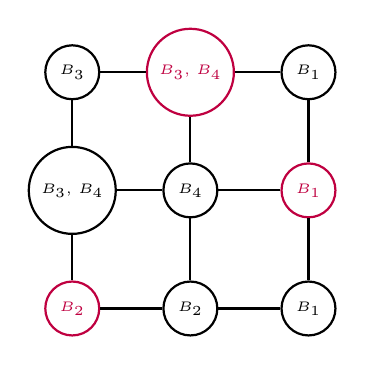
\begin{tikzpicture}[node distance={15mm}, thick, main/.style = {draw, circle}]
		\node[main] (1) {{\tiny $B_{3}$}};
		\node[main] (2) [right of=1] [color=purple] {{\tiny $B_{3}$, $B_{4}$}};
		\node[main] (3) [right of=2] {{\tiny $B_{1}$}};
		\node[main] (4) [below of=1] {{\tiny $B_{3}$, $B_{4}$}};
		\node[main] (5) [right of=4] {{\tiny $B_{4}$}};
		\node[main] (6) [right of=5] [color=purple] {{\tiny $B_{1}$}};
		\node[main] (7) [below of=4] [color=purple] {{\tiny $B_{2}$}};
		\node[main] (8) [right of=7] {{\tiny $B_{2}$}};
		\node[main] (9) [right of=8] {{\tiny $B_{1}$}};
		\path
			(1) edge (2) (2) edge (5)
			(2) edge (3) (3) edge (6)
			(1) edge (4) (5) edge (8)
			(4) edge (7) (6) edge (9)
			(4) edge (5) (5) edge (6)
			(7) edge (8) (8) edge (9);
	\end{tikzpicture}
	\caption{Brumble of a graph $G$.}
	\label{hit}
\end{figure}

\begin{lemma}[duality]
	If $(T, \beta)$ is a tree decomposition of $G$ and $\mathcal{B}$ is a bramble then $(\exists x \in V(T)) \beta(x)$ hits the bramble.
\end{lemma}

\begin{observ}
	If $(T, \beta)$ is a tree decomposition of $G$ and $F \subseteq G$ connected, then $\{x \in V(T) : \beta(x) \cap V(F) \neq \emptyset\}$ induces a connected subtree of $T$.
\end{observ}

\begin{proof}
	By induction on $|V(F)|$.
	
	\begin{enumerate}[(i)]
		\item $|V(F)| = 1$ is by the definition.
		\item $|V(F)| > 1$ consider $v \in V(F)$ such that $F - v$ is connected (we could take a leaf from a spanning tree of $F$) so we use an induction hypothesis $F - v$. We take a subtree on $V(F-b)$ and $\{v\}$. By the definition $\exists y: u,v \in \beta(y)$.
	\end{enumerate}
\end{proof}

\begin{proof}[Proof of lemma]
	For contradiction suppose it is false. So $(\forall x \in V(T)) \beta (x)$ does not hit $\mathcal{B}$ so we have $B_{x} \in \mathcal{B}$ disjoint from $\beta(x)$. By lemma $B_{x}$ forms in $(T, \beta)$ a connected subtree. Again we assign "arrows" to vertices pointing to $x$--$B_{x}$. Also there are more arrows than edges so at least one edge has two "arrows". We can find $B_{x}$ and $B_{x'}$ not in the same bag so they are disjoint. This is a contradiction by the definition.
\end{proof}

Note that on $K$ clique the bramble is $\mathcal{B} = \{\{u\}: u \in K\}$.

\begin{defn}
	\textbf{Order} of rumble is defined as $\text{order}(\mathcal{B}) = \min (|X|): X \text{ hits } \mathcal{B}$.
\end{defn} 

\begin{cor}
	$\text{tw}(G) \geq \max (\text{order}(\mathcal{B})) - 1$ for all $\mathcal{B}$ rumble in $G$.
\end{cor}

\begin{rem}
	It can be proven so that there is equality not inequality. But we will not be showing this result since it is not so easy.
\end{rem}

In other words we may rewrite the previous findings as a similiar lemma.

\begin{lemma}
	$\forall$ tree decompositions $(T, \beta)$ and $\forall$ bramble $\mathcal{B}$ in $G$ it holds that
	
	$$
	\text{width}(T, \beta) \geq \text{order}(\mathcal{B}) - 1
	$$
\end{lemma}

\subsection{$n \times n$ grid}

Now we will take a look at a simple example of a graph and its tree decomposition and bramble. This graph is an $n \times n$ grid where every neighbor is connected, one can be seen on picture \ref{nbynmatrix}.

\begin{figure}[!ht]\centering
	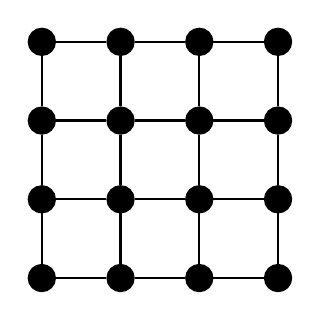
\begin{tikzpicture}[node distance={10mm}, thick, main/.style = {draw, circle, fill}]
		\node[main] (1) {};
		\node[main] (2) [right of=1] {};
		\node[main] (3) [right of=2] {};
		\node[main] (4) [below of=1] {};
		\node[main] (5) [right of=4] {};
		\node[main] (6) [right of=5] []{};
		\node[main] (7) [below of=4] []{};
		\node[main] (8) [right of=7] {};
		\node[main] (9) [right of=8] {};
		\node[main] (10) [below of=7] {};
		\node[main] (11) [right of=10] {};
		\node[main] (12) [right of=11] {};
		\node[main] (13) [right of=3] {};
		\node[main] (14) [right of=6] {};
		\node[main] (15) [right of=9] {};
		\node[main] (16) [right of=12] {};
		\path
			(1) edge (2) (2) edge (5) (14) edge (13)
			(2) edge (3) (3) edge (6) (14) edge (15)
			(1) edge (4) (5) edge (8) (15) edge (16)
			(4) edge (7) (6) edge (9) (7) edge (10)
			(4) edge (5) (5) edge (6) (8) edge (11)
			(7) edge (8) (8) edge (9) (9) edge (12)
			(10) edge (11) (11) edge (12)
			(12) edge (16) (9) edge (15)
			(6) edge (14) (3) edge (13);
	\end{tikzpicture}
	\caption{$n \times n$ matrix example.}
	\label{nbynmatrix}
\end{figure}

When we examine a tree decomposition we may easily find one such with tree width $2n$. That is we take 2 rows that are adjacent. But much better tree decomposition is when we take it like it is visualized on picture \ref{treewidthnbyn}. This gives us a tree decomposition with width $n+1$.

\begin{figure}[!ht]\centering
	\begin{subfigure}{0.25\textwidth}
		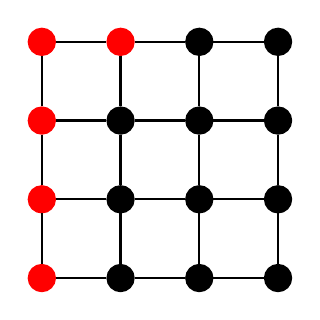
\begin{tikzpicture}[node distance={10mm}, thick, main/.style = {draw, circle, fill}]
			\node[main] (1) [color = red] {};
			\node[main] (2) [right of=1] [color = red] {};
			\node[main] (3) [right of=2] {};
			\node[main] (4) [below of=1] [color = red] {};
			\node[main] (5) [right of=4] {};
			\node[main] (6) [right of=5] {};
			\node[main] (7) [below of=4] [color = red] {};
			\node[main] (8) [right of=7] {};
			\node[main] (9) [right of=8] {};
			\node[main] (10) [below of=7] [color = red] {};
			\node[main] (11) [right of=10] {};
			\node[main] (12) [right of=11] {};
			\node[main] (13) [right of=3] {};
			\node[main] (14) [right of=6] {};
			\node[main] (15) [right of=9] {};
			\node[main] (16) [right of=12] {};
			\path
			(1) edge (2) (2) edge (5) (14) edge (13)
			(2) edge (3) (3) edge (6) (14) edge (15)
			(1) edge (4) (5) edge (8) (15) edge (16)
			(4) edge (7) (6) edge (9) (7) edge (10)
			(4) edge (5) (5) edge (6) (8) edge (11)
			(7) edge (8) (8) edge (9) (9) edge (12)
			(10) edge (11) (11) edge (12)
			(12) edge (16) (9) edge (15)
			(6) edge (14) (3) edge (13);
		\end{tikzpicture}
	\end{subfigure}
	\begin{subfigure}{0.25\textwidth}
		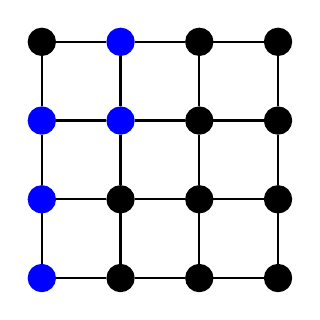
\begin{tikzpicture}[node distance={10mm}, thick, main/.style = {draw, circle, fill}]
			\node[main] (1) {};
			\node[main] (2) [right of=1] [color = blue] {};
			\node[main] (3) [right of=2] {};
			\node[main] (4) [below of=1] [color = blue] {};
			\node[main] (5) [right of=4] [color = blue] {};
			\node[main] (6) [right of=5] {};
			\node[main] (7) [below of=4] [color = blue] {};
			\node[main] (8) [right of=7] {};
			\node[main] (9) [right of=8] {};
			\node[main] (10) [below of=7] [color = blue] {};
			\node[main] (11) [right of=10] {};
			\node[main] (12) [right of=11] {};
			\node[main] (13) [right of=3] {};
			\node[main] (14) [right of=6] {};
			\node[main] (15) [right of=9] {};
			\node[main] (16) [right of=12] {};
			\path
			(1) edge (2) (2) edge (5) (14) edge (13)
			(2) edge (3) (3) edge (6) (14) edge (15)
			(1) edge (4) (5) edge (8) (15) edge (16)
			(4) edge (7) (6) edge (9) (7) edge (10)
			(4) edge (5) (5) edge (6) (8) edge (11)
			(7) edge (8) (8) edge (9) (9) edge (12)
			(10) edge (11) (11) edge (12)
			(12) edge (16) (9) edge (15)
			(6) edge (14) (3) edge (13);
		\end{tikzpicture}
	\end{subfigure}
	\begin{subfigure}{0.25\textwidth}
		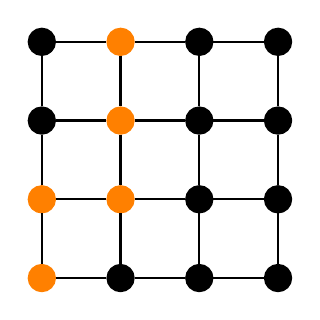
\begin{tikzpicture}[node distance={10mm}, thick, main/.style = {draw, circle, fill}]
			\node[main] (1) {};
			\node[main] (2) [right of=1] [color = orange] {};
			\node[main] (3) [right of=2] {};
			\node[main] (4) [below of=1] {};
			\node[main] (5) [right of=4] [color = orange] {};
			\node[main] (6) [right of=5] {};
			\node[main] (7) [below of=4] [color = orange] {};
			\node[main] (8) [right of=7] [color = orange] {};
			\node[main] (9) [right of=8] {};
			\node[main] (10) [below of=7] [color = orange] {};
			\node[main] (11) [right of=10] {};
			\node[main] (12) [right of=11] {};
			\node[main] (13) [right of=3] {};
			\node[main] (14) [right of=6] {};
			\node[main] (15) [right of=9] {};
			\node[main] (16) [right of=12] {};
			\path
			(1) edge (2) (2) edge (5) (14) edge (13)
			(2) edge (3) (3) edge (6) (14) edge (15)
			(1) edge (4) (5) edge (8) (15) edge (16)
			(4) edge (7) (6) edge (9) (7) edge (10)
			(4) edge (5) (5) edge (6) (8) edge (11)
			(7) edge (8) (8) edge (9) (9) edge (12)
			(10) edge (11) (11) edge (12)
			(12) edge (16) (9) edge (15)
			(6) edge (14) (3) edge (13);
		\end{tikzpicture}
	\end{subfigure}
	\caption{First three bags of tree decomposition.}
	\label{treewidthnbyn}
\end{figure}

So we can say that $\text{tw}(n \times n \text{grid}) \leq n$. Can we construct some with even lower width? We can use the previous lemma and construct a bramble which can be seen on picture \ref{bramblenbyn}. So there are two special setts on the sides and then we have all the crosses in the rest of the grid. This will lead to bramble $\mathcal{B}$ of order $\geq n+1$. We must select two points for two special sets and points on the diagonal for example. Therefore with the use of the lemma we also have that $\text{tw}(n \times n \text{grid}) \geq n$ thus it has to be equal.

\begin{figure}[!ht]\centering
	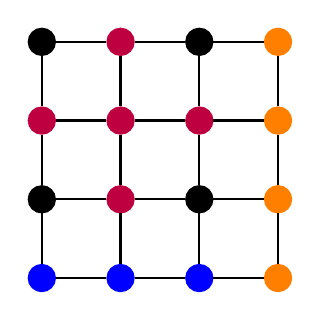
\begin{tikzpicture}[node distance={10mm}, thick, main/.style = {draw, circle, fill}]
		\node[main] (1) {};
		\node[main] (2) [right of=1] [color = purple] {};
		\node[main] (3) [right of=2] {};
		\node[main] (4) [below of=1] [color = purple] {};
		\node[main] (5) [right of=4] [color = purple] {};
		\node[main] (6) [right of=5] [color = purple] {};
		\node[main] (7) [below of=4] {};
		\node[main] (8) [right of=7] [color = purple] {};
		\node[main] (9) [right of=8] {};
		\node[main] (10) [below of=7] [color = blue] {};
		\node[main] (11) [right of=10] [color = blue] {};
		\node[main] (12) [right of=11] [color = blue] {};
		\node[main] (13) [right of=3] [color = orange] {};
		\node[main] (14) [right of=6] [color = orange] {};
		\node[main] (15) [right of=9] [color = orange] {};
		\node[main] (16) [right of=12] [color = orange] {};
		\path
		(1) edge (2) (2) edge (5) (14) edge (13)
		(2) edge (3) (3) edge (6) (14) edge (15)
		(1) edge (4) (5) edge (8) (15) edge (16)
		(4) edge (7) (6) edge (9) (7) edge (10)
		(4) edge (5) (5) edge (6) (8) edge (11)
		(7) edge (8) (8) edge (9) (9) edge (12)
		(10) edge (11) (11) edge (12)
		(12) edge (16) (9) edge (15)
		(6) edge (14) (3) edge (13);
	\end{tikzpicture}
	\caption{A bramble for $n \times n$ grid.}
	\label{bramblenbyn}
\end{figure}

With that we can state that if $n \times n$ grid $\leq_{m} G$ then $\text{tw}(G) \geq n$. Which also means that we can construct planar graph with any given tree width.

\begin{thm}
	$\text{tw}(G) \geq \Omega(n^{10})$ then $n \times n$ grid $\leq_{m} G$.
\end{thm}

This is quite recent discovery and long time it was only exponential. Now it is polynomial. We won't be proving this but instead we take a look at something in a way similiar.

\subsection{$n$-ladder}

$n$-ladder is graph that looks like a $2 \times n$ grid. Or just like it is on the picture \ref{nladder}.

\begin{figure}[!ht]\centering
	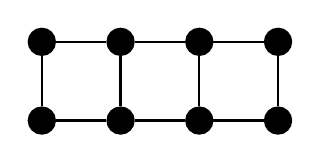
\begin{tikzpicture}[node distance={10mm}, thick, main/.style = {draw, circle, fill}]
		\node[main] (1) {};
		\node[main] (2) [right of=1] {};
		\node[main] (3) [right of=2] {};
		\node[main] (4) [below of=1] {};
		\node[main] (5) [right of=4] {};
		\node[main] (6) [right of=5] {};
		\node[main] (13) [right of=3] {};
		\node[main] (14) [right of=6] {};
		\path
		(1) edge (2) (2) edge (5)
		(2) edge (3) (3) edge (6)
		(1) edge (4) (13) edge (14)
		(4) edge (5) (5) edge (6)
		(6) edge (14) (3) edge (13);
	\end{tikzpicture}
	\caption{Example of an $n$-ladder.}
	\label{nladder}
\end{figure}

\begin{thm}
	$\text{tw}(G) \geq 2n^{2} - 1 \Rightarrow$ $n$-ladder $\leq_{m} G$.
\end{thm}

We won't be proving this straightforward. Instead we will prove something similiar which implies this theorem.

\begin{thm}
	If $G$ contains a bramble $\mathcal{B}$ of order $\geq 2n^2$ then $n$-ladder $\leq_{m} G$.
\end{thm}

Firstly we will show some lemmas.

\begin{lemma}
	If $\mathcal{B}$ is a bramble in $G$, then there exists path $P \subseteq G$ such that
	
	$$
	\forall B \in \mathcal{B} : B \cap V(P) \neq \emptyset
	$$
\end{lemma}

\begin{proof}
	Lets take $B_{1} \in \mathcal{B}$ and $x \in V(G)$ such that $x \in B_{1}$. If it is contained in all sets from bramble then we are done. Otherwise find such $B_{2} \in \mathcal{B}$ that does not contain it. Then by the bramble properties we are able to find path from $x$ to $B_{2}$. If now the path is contained in all sets from bramble we are done. Otherwise we iterate.
\end{proof}

\begin{lemma}
	Suppose $\mathcal{B}$ is a bramble, $\mathcal{B} = \mathcal{B}_{1} \dot \cup \mathcal{B}_{2}$. Then $\mathcal{B}_{1}$ and $\mathcal{B}_{2}$ are also brambles and
	
	$$
	\text{order}(\mathcal{B}) \leq \text{order}(\mathcal{B}_{1}) + \text{order}(\mathcal{B}_{2})
	$$
\end{lemma}

\begin{proof}
	This is straightforward from the definition of the bramble and some observations.
\end{proof}

\begin{proof}[Proof of theorem]
	Let $P$ be a path intersecting all sets in $\mathcal{B}$. let $P_{1}$ be a path segment.
	
	$$
	\mathcal{B}_{1} = \{B \in \mathcal{B} : B \cap V(P_{1} \neq \emptyset)\}
	$$
	
	Choose $P_{1}$ shortest such that $\text{order}(\mathcal{B}_{1}) \geq n^2$. We also claim there need to be equality since we are looking for the shortest path. Now let $\mathcal{B}_{2} = \mathcal{B} \setminus \mathcal{B}_{1}$. By the lemma we know $\text{order}(\mathcal{B}_{2}) \geq n^{2}$. Also we set $P_{2}$ to path intersecting all sets in $\mathcal{B}_{2}$.
	
	The claim is that $G$ contains $n^{2}$ disjoint paths from $P_{1}$ to $P_{2}$, By Merger's theorem if there is cut of such size there must as many disjoint paths. If we would remove $< n^{2}$ vertices there would exists in both paths such $B_{1}$ and $B_{2}$ respectively so the are not hit. By their properties they induce a connected subgraph. So there is a path. This proves the claim.
	
	We also remind ourselves a theorem
	
	\begin{thm}[Erdos-Szekeres]
		Every sequence of length $n^2$ contains a monotone sub-sequence of length $n$.
	\end{thm}
	
	Thus if the sub-sequence is increasing we just find $n$ paths thus an $n$-ladder. If it is decreasing we just flip one path and find the same result.
\end{proof}

Now we will see an application of this theorem.

\begin{thm}[Erdos-Prosa]
	There exists $f$ such that $\forall k$ $\forall G$ either
	
	\begin{itemize}
		\item $G$ contains more than $k$ pairwise distinct cycles or
		\item $\exists X \subseteq V(G)$, $|X| \leq f(X)$ such that $G - X$ does not contain cycle.
	\end{itemize}
\end{thm}

They proved it for $f(k) = O(k \log k)$, but we will show for other $f$ that exploits our previous theorem.

\begin{defn}
	$n_{1}, n_{2}, \dots, n_{m} \in \N$ is \textbf{$k$-bounded} if $n_{1}, n_{2}, \dots, n_{m} \leq k/2$ and $\sum_{i} n_{i} \leq k$.
\end{defn}

Now we set our $f$ to be: $f(0) =0$ and

$$
f(k) = 2(2k+2)^2 + \max_{I \ k-\text{bounded}} \sum_{i \in I} f(i).
$$

\begin{proof}
	Suppose $G$ contains $\leq k$ disjoint cycles. We will be proving this by induction on $k$.
	
	$$
	\mathcal{B} = \{B \subseteq V(G) : G[B] \text{ is connected, contains } > k/2 \text{ disjoint cycles}\}
	$$
	
	is a bramble. Any two $B_{1}$ and $B_{2}$ must intersect otherwise we have a contradiction with our assumption of not having $k$ cycles. If $\text{order}(\mathcal{B}) \geq 2(2k+2)^2$ then there is $2k+2$-ladder as a minor of $G$. This means there would be $k+1$ pairwise distinct cycles which is a contradiction.
	
	So $(\exists X : |X| < 2(2k+2)^2) X \text{ hits } \mathcal{B}$. Now take $G - X$ and denote their components as $K_{1}, K_{2}, \dots$. let $n_{i}$ be the number of pairwise distinct cycles in $K_{i}$. We may see that the sum $\sum n_{i} \leq k$ otherwise it is a contradiction with the assumption. And also $n_{i} \leq k/2$ for any $i$. Due to the bramble properties. Thus this sequence is $k$-bounded. Apply induction on components. We get $|X_{i}| \leq f(n_{i})$ by induction hypothesis. Thus
	
	$$
	G = (X \cup \bigcup_{i} X_{i}) \text{ is a forest and}
	$$
	
	$$
	|G - (X \cup \bigcup_{i} X_{i})| \leq f(k)
	$$
\end{proof}
	\chapter{Polynomials for graph theory}

\section{Basics}

We will introduce polynomials representing the graphs. Then we will look at what properties these polynoms have. But firstly we will look at some basics. Let $p(x_{1}, \dots, x_{n})$ be a polynomial on $n$ variables. One term $ax_{i}^{l} x_{j}^k \dots$ is called a \textbf{monomial}.

\begin{defn}
	The \textbf{total degree} of a monomial $x_{1}^{d_{!}} x_{2}^{d_{2}} \cdots x_{n}^{d_{n}}$ is the sum $d_{1} + d_{2} + \dots + d_{n}$.
\end{defn}

\begin{defn}
	Total degree of polynomial is the maximal total degree of its monomials.
\end{defn}

Also we will denote $[x_{1}^{d_{1}} \dots x_{n}^{d_{n}}]p$ the coefficients of $x_{1}^{d_{1}} \dots x_{n}^{d_{n}}$.

\begin{thm}[Chevalley–Warning, \textit{no proof}]
	Let $p$ be a prime number and $f_{1}, \dots, f_{k}$ polynomials over $\Z_{p}$ in $n$ variables and $\sum_{i = 1}^{k} \text{total degree of } f_{i} < n$, then the number of $a_{1}, \dots, a_{n} \in \Z_{p}$ such that for all $i$ $f_{i}(a_{1}, \dots, a_{n}) = 0$ is divisible by $p$.
\end{thm}

Now lets see an example of this. Let $f_{1} = x^2 + y^2 + z^2 + u =0$ and $f_{2} = x - y + z - u = 0$ over $\Z_{3}$. The total degree of $f_{1} + f_{2} = 2 + 1 < 4$ which is the number of variables. So the solutions are $x = y = z = u =0$ where the number of them has to be divisible by $3$. Also we have a solution $x = 1, z = 1, y = 2, u =0$.

\begin{thm}[Combinatorial Nullstellensatz, \textit{no proof}]
	Let $f$ be a polynomial in $n$ variables $x_{1}, \dots, x_{n}$, $f \not\equiv 0$. Suppose $S_{1}, S_{2}, \dots, S_{n} \subseteq \R$ such that $(\forall i) |S_{i}| > \deg_{x_{i}}(f)$. Then $\exists a_{1} \in S_{1}, \dots, a_{n} \in S_{n}$ such that $f(a_{1}, \dots, a_{n}) \neq 0$.
\end{thm}

Where $\deg_{x_{i}}(f)$ is the largest degree of $x_{i}$ in $f$. Example of application would be to ask if graph $G$ has a $3$-regular graphs as a subgraph, e.g. if it is true that $\delta(G) \geq 10^{10} \Rightarrow G$ has a $3$-regular subgraph? Generally NO.

\begin{thm}
	Suppose $\delta(G) \geq 4, \Delta(G) \leq 5$ and $G$ is not 4-regular. Then $G$ has a $3$-regular subgraph.
\end{thm}

\begin{proof}
	We will consider the following polynomials over $\Z_{3}$, for $v \in V(G)$ we define $f_{v} = \sum_{e \ni v} x_{e}^{2}$. Now we will take a look at such system of equations. We have this many variables: $|E(G)| = \frac{\sum_{v} \deg(v)}{2} > 2|V(G)|$. (Remember $G$ is not 4-regular.) And $\sum_{v} \text{total degree}(f_v) = 2|V(G)| < |E(G)|$. This implies that we can use the first theorem. Therefore $|\{a_{e} \in \Z_{3} : e \in E(G)\}|$ such that $f_{v}(\overrightarrow{a}) =0$ for all $v \in V(G)$ is divisible by 3. There exists at least one solution (since $x_{e} = 0$ for $e \in E(G)$) which means there exists another solution $\{a_{e} : e \in E(G)\}$ such that $\exists e : a_{e} \neq 0$.
	
	Now we create a subgraph $H$ as follows. $E(H) = \{e \in E(G) : a_{e} \neq 0\}$ and $V(H)$ are all vertices incident to $E(H)$. If we look at vertex $v$ then $f_{v}(\overrightarrow{a}) = \sum_{e \ni_{G} v} a_{e}^{2} = \sum_{e \ni_{H} v} a_{e}^{2}$ which is equivalent to $\deg_{H}(v) \mod 3$. Also $f_{v} = 0$. So every vertex has a degree 3.
\end{proof}

\section{List coloring polynomial}

Now we will use polynomials for coloring, but not the usual one we may find. We will be talking about a coloring which is obtained by choosing one color from a list assigned to each vertex. Then it must have the same property as a normal coloring. This is called \textbf{list coloring}. When all vertices have the same size lists $k$, than it can be also called that it is \textbf{$k$-choosable}.

\begin{defn}
	List chromatic number $\chi_{l}(G) = \text{smallest } k : G$ can be colored from any assignment of list of size $\geq k$.
\end{defn}

We will be trying to obtain the result that every bipartite plane graph is $3$ list colorable. But before we do so we will build another theory. Also it is possible to create such bipartite graphs that the $\chi_{l}(G)$ is arbitrarily large. For a graph $G$ we define $\overrightarrow{G}$ as an arbitrary orientation of $G$. And also we will define a polynomial:

$$
P_{\overrightarrow{G}} (x_{1}, \dots, x_{n}) = \prod_{(v_{i},v_{j}) \in E(\overrightarrow{G})} x_{i} - x_{j}
$$

To get a better understanding lets see a simple example of a graph $G$ which can be seen on a picture \ref{pol-ex}. Here the polynomial would be $P_{\overrightarrow{G}} = (x_{2} - x_{1}) (x_{3} - x_{2}) (x_{1} - x_{3}) = x_1 x_2 x_3 - x_2 x_3 - x_1 x_2^2 + x_2^2 x_3 - x_1^2 x_3 + x_1 x_3^2 + x_1^2 x_2 - x_1x_2x_3$.

\begin{figure}[!ht]\centering
	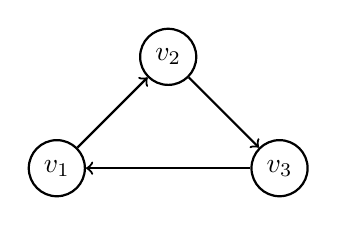
\begin{tikzpicture}[node distance={20mm}, thick, main/.style = {draw, circle}]
		\node[main] (2) {$v_{2}$};
		\node[main] (1) [below left of=2] {$v_{1}$};
		\node[main] (3) [below right of=2] {$v_{3}$};
		\path[->] (1) edge (2)
				  (2) edge (3)
				  (3) edge (1);
	\end{tikzpicture}
	\caption{Example for a polynomial for a graph $\overrightarrow{G}$.}
	\label{pol-ex}
\end{figure}

Now if we take $V(G) = \{v_{1}, \dots, v_{n}\}$ which map each one of them $v_{i} \to x_{i}$. Then for an assignment $\overrightarrow{c}$ as for each $i$ $v_i \to c_i$ we know that $G$ has a proper coloring iff $P_{\overrightarrow{G}}(\overrightarrow{c}) \neq 0$. That is if $S_{1}, \dots, S_{n}$ are lists of allowed colors for $v_{1}, \dots, v_{n}$ then $G$ is colorable from $S_{1}, \dots, S_{n}$ iff $(\exists c_{1} \in S_{1}, \dots, c_{n} \in S_{n}) P_{\overrightarrow{G}}(c_{1}, \dots, c_{n}) \neq 0$. To prove this we could use the same theorem, but we will need a stronger version.

\begin{thm}[Combinatorial Nullstellensatz 2nd version]
	Let $f$ be a polynomial in $x_{1}, \dots, x_{n}$ and $S_{1}, \dots, S_{n} \subseteq \R$. If $(\exists d_{1}, \dots, d_{n})$ total degree $(f) \leq d_{1} + \dots + d_{n}$ and $[x_{1}^{d_{1}}\dots x_{n}^{d_{n}}]f \neq 0$ and $(\forall i) |S_{i}| > d_{i}$. Then $\exists c_{1} \in S_{1}, \dots, c_{n} \in S_{n} : f(c_{1}, \dots, c_{n}) \neq 0$.
\end{thm}

But why does it hold? We can assume $|S_{i}| = d_{i} + 1$. For the values $S_{i} = \{a_{1}, \dots, a_{d_{i}+1}\}$ (as colors). We know that if $x_{i} \in S$ then $(x_{i} - a_{1}) (x_{i} - a_{2}) \cdots (x_{i} - a_{d_{i}+1}) = 0$. Then $x_{i}^{d+1} - (a_{1} + \dots + a_{d+1}) x_{i}^{d_{i}} + \dots$ where we denote $b_{d_{i}} = (a_{1} + \dots + a_{d+1})$ so that leads to:

$$
x_{i}^{d_{i}+1} = b_{d_{i}}x_{i}^{d_{i}} + \dots + b_{1}x_{1} + b_{0}
$$

Now we may take a polynomial $f$ from the 2nd theorem. The polynomial $f'$ has the same values on $S_{1}, \dots, S_{n}$ but $\deg_{v_{i}}(f') \leq d_{i}$. So now the condition $(\forall i) |S_{i}| > \deg_{v_{i}} (f')$ holds. Only thing is to see that $f' \not\equiv 0$.

We have already shown this theorem.

\begin{thm}
	If $[x_{1}^{d_1} \dots x_{n}^{d_n}]P \neq 0$, $d_1 + \dots + d_n = $ total degree of $P$, $S_1, \dots, S_{n}, (\forall i) |S_i| > d_i$ then $\Rightarrow (\exists c_{1} \in S_{1}, \dots, c_{n} \in S_{n}) P(c_{1}, \dots c_n) \neq 0$.
\end{thm}

\begin{observ}
	$P_{\overrightarrow{G}} (c_1, \dots, c_n) \neq 0 \Leftrightarrow c_1, \dots, c_n$ is a proper coloring of $G$.
\end{observ}

By combining these two results we may get a following corollary.

\begin{cor}
	If $[x_{1}^{d_1} \dots x_{n}^{d_n}]P_{\overrightarrow{G}} \neq 0$ and $L$ is a list assignment such that $(\forall i) |L(v_i)| > d$ then $G$ is $L$-colorable.
\end{cor}

Now we will see other variants of this polynomial and how it can be computed in other ways. Here we see an example on picture \ref{orientation}. First we may see the original graph and its orientation $\overrightarrow{G}$ on picture \ref{orientation-original}. Then one monomial in a corresponding polynomial is a choice of one $\pm x_{i}$ in the bracket. This choice induces a new orientation $\overrightsimarrow{G}$ which both can be seen on picture \ref{orientation-choice}. Thus the polynomial can be computed as follows:

$$
\sum_{\overrightsimarrow{G} \text{ orientation of }G} (-1)^{\text{\# of different direction in } \overrightsimarrow{G} \text{ from } \overrightarrow{G}} \prod_{i} x_{i}^{\deg^{-}_{\overrightsimarrow{G}}(v_{i})}
$$

\begin{figure}[!ht]\centering
	\begin{subfigure}{0.45\textwidth}\centering
		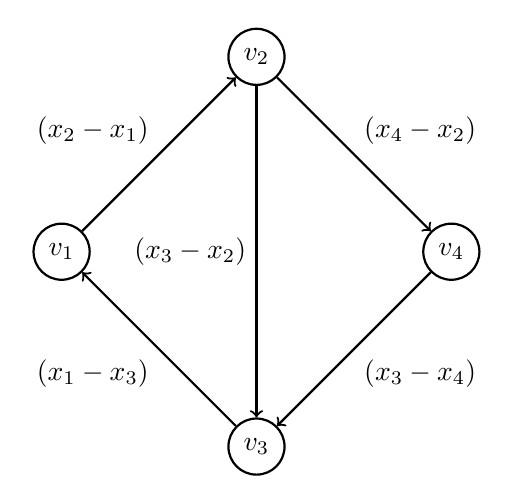
\begin{tikzpicture}[node distance={35mm}, thick, main/.style = {draw, circle}]
			\node[main] (1) {$v_{1}$};
			\node[main] (2) [above right of=1] {$v_{2}$};
			\node[main] (3) [below right of=1] {$v_{3}$};
			\node[main] (4) [above right of=3] {$v_{4}$};
			\draw[->] (1) -- (2) node[midway, above left] {$(x_{2} - x_{1})$};
			\draw[->] (3) -- (1) node[midway, below left] {$(x_{1} - x_{3})$};
			\draw[->] (2) -- (3) node[midway, left] {$(x_{3} - x_{2})$};
			\draw[->] (2) -- (4) node[midway, above right] {$(x_{4} - x_{2})$};
			\draw[->] (4) -- (3) node[midway, below right] {$(x_{3} - x_{4})$};
		\end{tikzpicture}
		\caption{The original graph $\overrightarrow{G}$.}
		\label{orientation-original}
	\end{subfigure}
	\begin{subfigure}{0.45\textwidth}\centering
		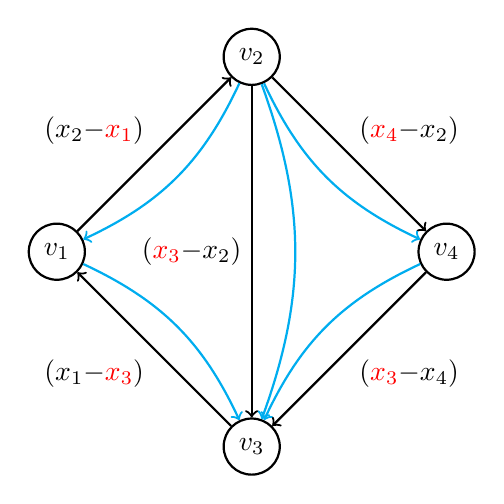
\begin{tikzpicture}[node distance={35mm}, thick, main/.style = {draw, circle}]
			\node[main] (1) {$v_{1}$};
			\node[main] (2) [above right of=1] {$v_{2}$};
			\node[main] (3) [below right of=1] {$v_{3}$};
			\node[main] (4) [above right of=3] {$v_{4}$};
			\draw[->] (1) -- (2) node[midway, above left] {$(x_{2} -$\textcolor{red}{$x_{1}$}$)$};
			\draw[->] (3) -- (1) node[midway, below left] {$(x_{1} -$\textcolor{red}{$x_{3}$}$)$};
			\draw[->] (2) -- (3) node[midway, left] {$($\textcolor{red}{$x_{3}$}$ - x_{2})$};
			\draw[->] (2) -- (4) node[midway, above right] {$($\textcolor{red}{$x_{4}$}$ - x_{2})$};
			\draw[->] (4) -- (3) node[midway, below right] {$($\textcolor{red}{$x_{3}$}$ - x_{4})$};
			\draw[->, bend left=20, color=cyan] (2) edge (1);
			\draw[->, bend right=20, color=cyan] (2) edge (4);
			\draw[->, bend right=20, color=cyan] (4) edge (3);
			\draw[->, bend left=20, color=cyan] (2) edge (3);
			\draw[->, bend left=20, color=cyan] (1) edge (3);
		\end{tikzpicture}
		\caption{The \textcolor{red}{choice} and \textcolor{cyan}{new orientation $\overrightsimarrow{G}$}.}
		\label{orientation-choice}
	\end{subfigure}
	\caption{Example for computing polynomial by orientation, the original graph $\overrightarrow{G}$.}
	\label{orientation}
\end{figure}

Thus altogether we get this result:

$$
[x_{1}^{d_{1}} x_{2}^{d_{2}} \dots x_{n}^{d_{n}}]P_{\overrightarrow{G}} = \sum_{\overrightsimarrow{G} \text{ orientation of }G : \deg^{-}_{\overrightsimarrow{G}}(v_{i}) = d_{i} \forall i} (-1)^{\text{\# of different direction in } \overrightsimarrow{G} \text{ from } \overrightarrow{G}}
$$

When we show another example where we have a vertex with in degree 3. See picture \ref{eulerian-orientation}. For the indegree to be same it must be that for all changed edge to the vertex there must be some changed edge out of the vertex.

\begin{figure}[!ht]\centering
	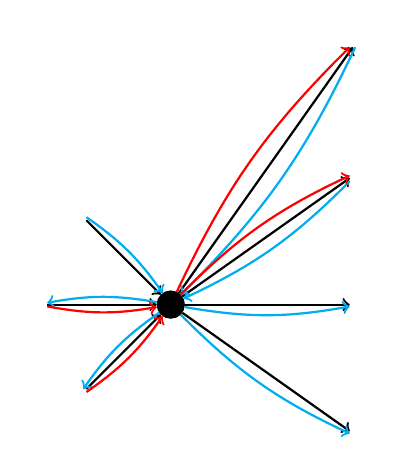
\begin{tikzpicture}[node distance={17mm}, thick, main/.style = {draw, circle}]
		\node (R1) {};
		\node [below of=R1] (R2) {};
		\node [below of=R2] (R3) {};
		\node [below of=R3] (R4) {};
		\node[main, fill] [below left of=R2] [above left of=R3] (1) {};
		\node [above left of=1] (L1) {};
		\node [left of=1] (L2) {};
		\node [below left of=1] (L3) {};
		\draw[->] (L1) edge (1);
		\draw[->] (L2) edge (1);
		\draw[->] (L3) edge (1);
		\draw[->] (1) edge (R1);
		\draw[->] (1) edge (R2);
		\draw[->] (1) edge (R3);
		\draw[->] (1) edge (R4);
		\draw[->, bend left=10, color=cyan] (L1) edge (1);
		\draw[->, bend right=10, color=cyan] (1) edge (L2);
		\draw[->, bend right=10, color=cyan] (1) edge (L3);
		\draw[->, bend left=10, color=cyan] (R1) edge (1);
		\draw[->, bend left=10, color=cyan] (R2) edge (1);
		\draw[->, bend right=10, color=cyan] (1) edge (R3);
		\draw[->, bend right=10, color=cyan] (1) edge (R4);
		\draw[->, bend left=10, color=red] (1) edge (R1);
		\draw[->, bend left=10, color=red] (1) edge (R2);
		\draw[->, bend right=10, color=red] (L3) edge (1);
		\draw[->, bend right=10, color=red] (L2) edge (1);
	\end{tikzpicture}
	\caption{Example for Eulerian subgraph orientations.}
	\label{eulerian-orientation}
\end{figure}


\begin{observ}
	If $\overrightarrow{G}$ and $\overrightsimarrow{G}$ are orientations with the same indegrees, the $\overrightarrow{H}$ subgraph of $\overrightarrow{G}$ with edges oriented differently, then $\forall v \in V$ $\deg_{\overrightarrow{H}}^{+} (v) = \deg_{\overrightarrow{H}}^{-} (v)$ or in other words: $\overrightarrow{H}$ is Eulerian subgraph of $\overrightarrow{G}$.
\end{observ}

\begin{lemma}
	Suppose $\overrightarrow{G}$ is an orientation of $G$ such that $\forall i$ $d_{i} = \deg^{-}(v_{i})$ in $\overrightarrow{G}$. Then
	
	$$
	[x_{1}^{d_{1}} x_{2}^{d_{2}} \dots x_{n}^{d_{n}}] P_{\overrightarrow{G}} = \sum_{\overrightarrow{H} \text{ Eulerian subgraph of } \overrightarrow{G}} (-1)^{\left| E \left( \overrightarrow{H} \right) \right|}
	$$
	
	which is also equivalent to the \textbf{number of Eulerian paths of $\overrightarrow{G}$ with even number of edges} minus \textbf{number of Eulerian paths of $\overrightarrow{G}$ with odd number of edges}.
\end{lemma}

\begin{cor}
	Suppose $\overrightarrow{G}$ is an orientation of $G$ where $(\forall i) \deg^{-}(v_{i}) = d_{i}$. Let $L$ be a list assignment for $G$ s.t. $(\forall i) |L(v_{i})| > d_{i}$. If $\overrightarrow{G}$ has different number of Eulerian subgraphs with even and odd number of edges then it is $L$-colorable.
\end{cor}

Lets see this result on an example on pictures \ref{euler-list}. Where the sizes of lists are written in the nodes. We may see there are visualized two Eulerian paths with \textcolor{blue}{3} edges and \textcolor{orange}{4} edges. Also there is an empty Eulerian subgraph. Altogether we have two even subgraphs and one odd, so that means there exists $L$-coloring. But this theory only show the existence, not the construction.

\begin{figure}[!ht]\centering
	\begin{subfigure}{0.30\textwidth}\centering
		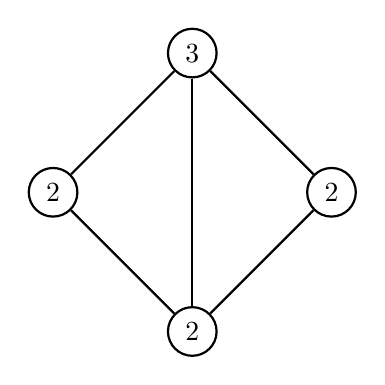
\begin{tikzpicture}[node distance={25mm}, thick, main/.style = {draw, circle}]
			\node[main] (1) {2};
			\node[main] (2) [above right of=1] {3};
			\node[main] (3) [below right of=1] {2};
			\node[main] (4) [above right of=3] {2};
			\draw (1) -- (2);
			\draw (3) -- (1);
			\draw (2) -- (3);
			\draw (2) -- (4);
			\draw (4) -- (3);
		\end{tikzpicture}
		\caption{The original graph $G$.}
	\end{subfigure}
	\begin{subfigure}{0.30\textwidth}\centering
		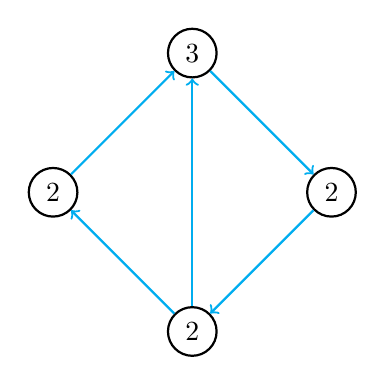
\begin{tikzpicture}[node distance={25mm}, thick, main/.style = {draw, circle}]
			\node[main] (1) {2};
			\node[main] (2) [above right of=1] {3};
			\node[main] (3) [below right of=1] {2};
			\node[main] (4) [above right of=3] {2};
			\draw[->, color=cyan] (1) -- (2);
			\draw[->, color=cyan] (3) -- (1);
			\draw[->, color=cyan] (3) -- (2);
			\draw[->, color=cyan] (2) -- (4);
			\draw[->, color=cyan] (4) -- (3);
		\end{tikzpicture}
		\caption{The orientation $\overrightarrow{G}$.}
	\end{subfigure}
	\begin{subfigure}{0.30\textwidth}\centering
		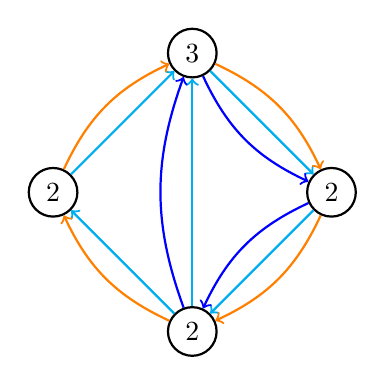
\begin{tikzpicture}[node distance={25mm}, thick, main/.style = {draw, circle}]
			\node[main] (1) {2};
			\node[main] (2) [above right of=1] {3};
			\node[main] (3) [below right of=1] {2};
			\node[main] (4) [above right of=3] {2};
			\draw[->, color=cyan] (1) -- (2);
			\draw[->, color=cyan] (3) -- (1);
			\draw[->, color=cyan] (3) -- (2);
			\draw[->, color=cyan] (2) -- (4);
			\draw[->, color=cyan] (4) -- (3);
			% First eulerian path.
			\draw[->, bend left=20, color=orange] (1) edge (2);
			\draw[->, bend left=20, color=orange] (3) edge (1);
			\draw[->, bend left=20, color=orange] (2) edge (4);
			\draw[->, bend left=20, color=orange] (4) edge (3);
			% Eulerian path second.
			\draw[->, bend left=20, color=blue] (3) edge (2);
			\draw[->, bend right=20, color=blue] (2) edge (4);
			\draw[->, bend right=20, color=blue] (4) edge (3);
		\end{tikzpicture}
		\caption{Euler subgraphs.}
	\end{subfigure}
	\caption{Usage of shown corollary for a list assignment.}
	\label{euler-list}
\end{figure}

Now lets take $G$ a bipartite graph. We may see an observation that every Eulerian subgraph is edge-disjoint union of cycles. Therefore if $G$ is bipertite, then it has even number of edges in all Eulerian subgraphs.

\begin{cor}
	If $G$ is bipartite, $\overrightarrow{G}$ has indegrees $d_{1}, \dots, d_{n}$ then $G$ is $L$-colorable for every list assignments $L$ s.t. $(\forall i) |L(v_{i})| > d_{i}$.
\end{cor}

\begin{observ}
	Every planar bipartite graph has an orientation with maximal indegree $\leq 2$ therefore it has list chromatic number at most 3.
\end{observ}

But it does not apply for all bipartite graphs since it is possible to create such bipartite graph such that $\chi_{l}$ is arbitrarily large.
	\chapter{VC - dimension}

VC stands for the names Varnik--Cherrorenkis. We will be considering a set systems $\mathcal{F}$. And then for a set $X$ we denote $X \cap \mathcal{F}$ as $\{X \cap A : A \in \mathcal{F}\}$.

\section{Set systems}

\begin{defn}
	$\mathcal{F}$ \textbf{breaks} $X$ if $X \cap \mathcal{F} = 2^{X}$.
\end{defn}

Lets see for ourselves an example, which is on picture \ref{broken-x}. For $\mathcal{F}$ we have all half planes in $\R^2$. Then the set $X = \{a,b,c\}$. Then if we draw all lines and choose both planes it will generate $X \cap \mathcal{F} = \{ \emptyset, \{a\}, \{b\}, \{c\}, \{a,b\}, \{b,c\}, \{a,c\}, \{a,b,c\}\}$ which are all subsets of $X$. Hence it breaks the $X$.

\begin{figure}[!ht]\centering
	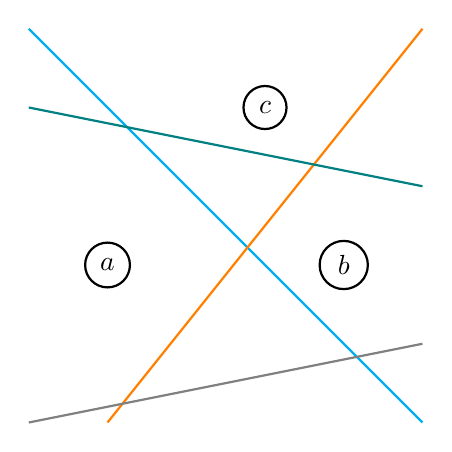
\begin{tikzpicture}[node distance={15mm}, thick, main/.style = {draw, circle}]
		\draw[color=cyan] (0,5) -- (5,0);
		\draw[color=orange] (1, 0) -- (5, 5);
		\draw[color=teal] (0,4) -- (5,3);
		\draw[color=gray] (0,0) -- (5, 1);
		\node[main] at (1, 2) {$a$};
		\node[main] at (4, 2) {$b$};
		\node[main] at (3, 4) {$c$};		
	\end{tikzpicture}
	\caption{Example of $\mathcal{F}$ and set $X$ which is broken.}
	\label{broken-x}
\end{figure}

\begin{defn}
	We say that $VC-\dim(\mathcal{F})$ is $\max \{|X| : \mathcal{F} \text{ breaks } X\}$.
\end{defn}

In our previous example we see that $VC-\dim(\mathcal{F})$ is at least 3. But we may see that it is exactly 3. Because if we take 4 points they are either all in convex hull thus it is impossible to take the opposite points or one point is in the convex hull of other three of them, for which it is impossible to take only the points forming the convex hull except the middle one. Other example can be $\mathcal{F}$ as all intervals in $\R$ for which the $VC-\dim(\mathcal{F})$ is 2.

All these examples are geometrical ones. Lets see some for graph theory. Lets have $G$ graph s.t. $K_{n} \nleq_{t} G$. Then $\mathcal{F} = \{N_{G}[v] : v \in V(G)\}$. Where the \textbf{closed neighborhood} is defined as $N_{G}[v] = \{v\} \cup \{u \mid \{u,v\} \in E(G)\}$. We may see that $VC-\dim(\mathcal{F}) \leq n-1$. For contradiction $X \subseteq V$ and $|X| = n$. For every 2-element subset there is a vertex adjacent to them, this would give me a $K_{n}$ as a topological subgraph.

\section{Subsystems}

Now we will be considering sub-systems. That is $\mathcal{F} \subseteq 2^{Y}$ for some $Y$. There will be defined a measurement $\mu$ on $Y$. As an example can be the half-planes but only inside the square of size 1.

\begin{defn}
	$N \subseteq Y$ is an $\epsilon$-net if
	
	$$
	(\forall A \in \mathcal{F}) : \mu(A) \geq \epsilon \mu(Y) \Rightarrow N \cap A \neq \emptyset
	$$
\end{defn}

For an example consider $\mathcal{F} = \{\text{axis aligned rectangles in }Y\}$ and $\mu$ be the area of the rectangle. Then the $\epsilon$-net must hit all rectangles. We can easily create a grid of points which are $\epsilon$ apart. This will create $\frac{1}{\epsilon^2}$ points in net.

\begin{thm}
	There $\exists c$ s.t. if $\mathcal{F} \subseteq 2^Y$ has $VC-\dim(\mathcal{F}) \leq k$ then
	
	$$
	(\forall \epsilon > 0) \quad c \cdot \frac{k}{\epsilon} \cdot \log \left( \frac{k}{\epsilon} \right)
	$$
	
	independently at random chosen elements of $Y$ form an $\epsilon$-net with probability $\geq 1/2$. This is all with the probability for $A \subseteq Y$ $\Pr [p \in A] = \frac{\mu(A)}{\mu(Y)}$.
\end{thm}

\begin{defn}
	$\tau (\mathcal{F}) = \min \left( |Z| : (\forall A \in \mathcal{F}) Z \cap A \neq \emptyset \right)$.
\end{defn}

As an example we may see that for $\mathcal{F}$ closed neighborhood in $G$ the $\tau(\mathcal{F})$ is for the minimal size of dominating set in the given graph $G$. Also we have shown that if $K_{k} \nleq_{t} G \Rightarrow VC-\dim(\mathcal{F}) \leq k - 1$.

Now we will introduce an integer program that will be able to solve this problem. Note that we will assume that $\mathcal{F}$ and $Y$ are finite. Otherwise it would not make any sense.

$$
\begin{aligned}
	&\min \sum_{v} x_{v} \\
	\forall v \in Y: \quad & x_{v} \in \{0,1\} \\
	\forall F \in \mathcal{F}: \quad & \sum_{v \in F} x_{v} \geq 1
\end{aligned}
$$

This problem will output such $X = \{x_{v} \mid v \in Y : x_{v} = 1\}$ and $|X| = \tau(\mathcal{F})$. We can use this to create an LP relaxation.

$$
\begin{aligned}
	&\min \sum_{v} x_{v} \\
	\forall v \in Y: \quad & x_{v} \geq 0 \\
	\forall F \in \mathcal{F}: \quad & \sum_{v \in F} x_{v} \geq 1
\end{aligned}
$$

We will denote this fraction optimum as $\tau^{\ast}(\mathcal{F})$. Easily seen it is $\leq \tau(\mathcal{F})$. And it is also solvable in polynomial time, due to the properties of linear programs. Now consider $\mathcal{F}$ which has $VC-\dim(\mathcal{F}) \leq k$. We then have $x_{v} : v \in Y$ from the optimal solution of LP. Lets put the measurement for all $A \subseteq Y: \mu(A) = \sum_{v \in A} x_{v}$. By the given solution we have that $F \in \mathcal{F}: \mu(F) \geq 1$. Also $\mu(Y) = \tau^{\ast}(\mathcal{F})$. Let $N$ be an $\epsilon$-net for $\epsilon = 1/\tau^{\ast}(\mathcal{F})$. That is because $N \cap F \neq 0$ for all $F \in \mathcal{F}$ s.t. $\mu(F) \geq \epsilon \mu(Y) = 1$. Therefore

$$
\tau(\mathcal{F}) \leq |N| = \Theta (k \tau^{\ast}(\mathcal{F}) \log(k \tau^{\ast}(\mathcal{F})))
$$

so it is $(k \log(k \tau^{\ast}(\mathcal{F})))$-approximation.
	\chapter{Edge disjoint spanning trees}

We will be trying to take a look at a problem of finding many edge disjoint spanning trees like on picture \ref{span-trees}. Note that this may be used in a technical problems like packet routing in a computer network. Since it can be done by finding a spanning tree and then path between two vertices is uniquely determined. But what if some edge breaks and it is not operating. Then you may choose another spanning tree.

\begin{figure}[!ht]\centering
	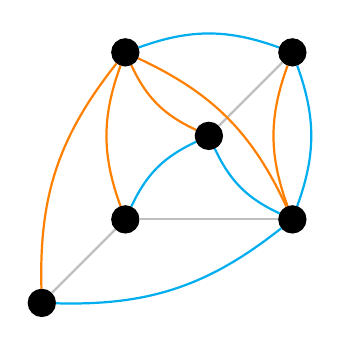
\begin{tikzpicture}[node distance={15mm}, thick, main/.style = {draw, circle, thick, fill}]
		\node[main] (1) {};
		\node[main, above right of = 1] (2) {};
		\node[main, below left of = 1] (3) {};
		\node[main, below right of = 2] (4) {};
		\node[main, above right of = 2] (5) {};
		\node[main, above left of = 2] (6) {};
		\path[color=lightgray] (3) edge (1) (1) edge (4) (2) edge (5);
		\path[color=cyan, thick, bend right = 20] (2) edge (1) (2) edge (4) (4) edge (5) (3) edge (4) (5) edge (6);
		\path[color=orange, bend right = 20] (6) edge (3) (6) edge (1) (6) edge (2) (4) edge (6) (5) edge (4);
	\end{tikzpicture}
	\caption{Example of two pairwise edge-disjoint spanning trees.}
	\label{span-trees}
\end{figure}

The terminology will be for a graph $G = (V,E)$. And the question is: Does $G$ have $k$ pairwise edge-disjoint spanning trees? Easily observable then if it happens than the graph $G$ is $k$-edge-connected. But does the other implication work? Well as it can be shown on picture \ref{counterexample-for-connectivity} no. But there is someway similiar result.

\begin{figure}[!ht]\centering
	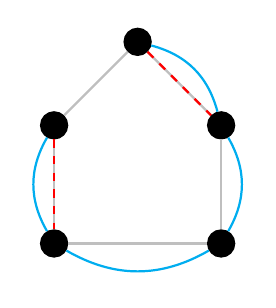
\begin{tikzpicture}[node distance={15mm}, thick, main/.style = {draw, circle, thick, fill}]
		\node[main] (1) {};
		\node[main, below right of = 1] (2) {};
		\node[main, below left of = 1] (3) {};
		\node[main, below of = 2] (4) {};
		\node[main, below of = 3] (5) {};
		\path[color=lightgray] (1) edge (2) (2) edge (4) (4) edge (5) (5) edge (3) (3) edge (1);
		\draw[color=red, dashed] (1) edge (2);
		\draw[color=red, dashed] (3) edge (5);
		\path[color=cyan, bend left = 30] (1) edge (2) (2) edge (4) (4) edge (5) (5) edge (3);
	\end{tikzpicture}
	\caption{Simple cycle for a counterexample. It is 2-edge-connected, but only 1 pairwise edge-disjoint spanning tree can be found. There is an example of a \textcolor{red}{edge-cut} and a \textcolor{cyan}{spanning tree}.}
	\label{counterexample-for-connectivity}
\end{figure}

\begin{thm}
	If $G$ is $2k$-edge-connected then $G$ has $k$ pairwise edge-disjoint spanning trees.
\end{thm}

This is similiar with what we have said before, only it is multiplied by 2. We will prove this by another theorem, which will be shown later on.

\section{Necessary condition}

Let $G$ be a graph with $k$ spanning trees. Then denote $\mathcal{P}$ as any division of vertices $V(G)$. That is $\bigcup_{P \in \mathcal{P}} P = V(G)$ and for two sets $P \neq Q \in \mathcal{P}$ it holds that $P \cap Q = \emptyset$. Then we will contract these sets into one vertex and then for every spanning tree there must remain $|\mathcal{P}| -1$ number of edges. So lets denote $e(\mathcal{P})$ as the number of edges of $G$ with ends in different parts of $\mathcal{P}$.

Now to observe that if $G$ has $k$ pairwise edge-disjoint spanning trees then for every $\mathcal{P}$ partition of $V(G)$ it holds that $e(\mathcal{P}) \geq k (|\mathcal{P}| - 1)$. This may be easily seen, but what about the second implication. There exists a Nash-Williams theorem which states exactly that. And we will be showing that.

\begin{observ}
	If $G$ is $2k$-edge-connected graph and then $G/\mathcal{P}$ is also $2k$-edge-connected then the minimal degree $\delta(G/\mathcal{P}) \geq 2k$ which implies that
	
	$$
	e(\mathcal{P}) = |E(G/\mathcal{P})| \geq \frac{1}{2} |\mathcal{P}| 2k = k |\mathcal{P}| > k (|\mathcal{P}| - 1)
	$$
\end{observ}

Where notation $G / \mathcal{P}$ is for contracting the partitions. Also we may see that this proves the former theorem. Now we will state and prove the theorem.

\begin{thm}
	$(\forall \mathcal{P} : \text{ partition of } V(G)) \ e(\mathcal{P}) \geq l (|\mathcal{P}| - 1)$ then there is $k$ pairwise edge-disjoint spanning trees.
\end{thm}

\begin{defn}
	Spanning forest is a set of edges that cover all vertices and is a forest.
\end{defn}

\begin{defn}
	\textbf{Jungle} is a set of $k$ pairwise edge-disjoint spanning forests.
\end{defn}

\begin{defn}
	For two jungles $J,J'$ in a graph $G$ and a subgraph $A \subseteq G$ we define a relation $J \cong_{A} J'$ if
	
	$$
	(\forall i) \ E(F_{i}) \setminus E(A) = E(F_{i}') \setminus F(A)
	$$
	
	and components of $F_{i} \cap A$ must be the same as in $F_{i}' \cap A$.
\end{defn}

\begin{figure}[!ht]\centering
	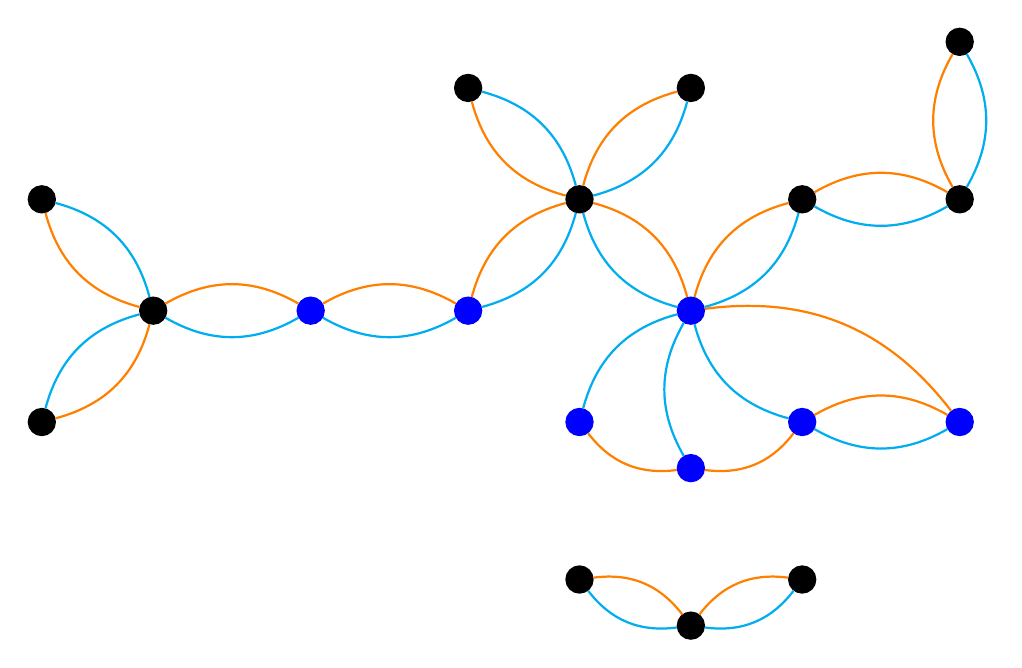
\begin{tikzpicture}[node distance={20mm}, thick, main/.style = {draw, circle, thick, fill}]
		\node[main] (1) {};
		\node[main, above left of = 1] (2) {};
		\node[main, below left of = 1] (3) {};
		\node[main, right of = 1, color=blue] (4) {};
		\node[main, right of = 4, color=blue] (5) {};
		\node[main, above right of = 5] (6) {};
		\node[main, above left of = 6] (7) {};
		\node[main, above right of = 6] (8) {};
		\node[main, below right of = 6, color=blue] (9) {};
		\node[main, below left of = 9, color=blue] (10) {};
		\node[main, below of = 9, color=blue] (11) {};
		\node[main, below right of = 9, color=blue] (12) {};
		\node[main, right of = 12, color=blue] (13) {};
		\node[main, above right of = 9] (14) {};
		\node[main, right of = 14] (15) {};
		\node[main, above of = 15] (16) {};
		\node[main, below of = 10] (17) {};
		\node[main, below of = 11] (18) {};
		\node[main, below of = 12] (19) {};
		\path[color=cyan, bend right] (1) edge (2)
			(1) edge (3) (1) edge (4) (4) edge (5)
			(5) edge (6) (6) edge (7) (6) edge (8)
			(6) edge (9) (9) edge (10) (9) edge (11)
			(9) edge (12) (9) edge (14) (14) edge (15)
			(15) edge (16) (17) edge (18) (18) edge (19)
			(12) edge (13);
		\path[color=orange, bend left] (1) edge (2)
			(1) edge (3) (1) edge (4) (4) edge (5)
			(5) edge (6) (6) edge (7) (6) edge (8)
			(6) edge (9) (9) edge (13) (12) edge (13)
			(12) edge (11) (11) edge (10) (14) edge (15)
			(15) edge (16) (17) edge (18) (18) edge (19)
			(9) edge (14);
	\end{tikzpicture}
	\caption{Example of two jungles, where \textcolor{cyan}{first} $J$ and \textcolor{orange}{second} $J'$ are $J \cong_{A} J'$ for \textcolor{blue}{vertices} in $A$.}
\end{figure}

\begin{defn}
	For a graph $G$, subgraph $A \subseteq G$ and a jungle $J$. $A$ is $J$-free if $(\forall e \in E(A))$ there exists a jungle $J' \cong J$ such that $e \notin E(\bigcup J')$. 
\end{defn}

\begin{proof}
	Lets take a jungle $J = (F_{1}, F_{2}, \dots, F_{k})$ in $G$ with $|E (\bigcup J)|$ largest possible. Before we continue we state a lemma.
	
	\begin{lemma}
		$\exists H \subseteq G$ connected such that $|V(H)| \geq 2$ and $(\forall i) H \cap F_{i}$ is connected (where $F_{i}$ is taken from jungle $J$).
	\end{lemma}
	
	\begin{proof}[Proof of lemma]
		We will take $A \subseteq G$ and two jungles $J = (F_{1}, \dots, F_{k}), J' = (F_{1}', \dots, F_{k}')$ in $G$. Let us choose $H \subseteq G$ connected which is $J$-free and maximal. We take $\mathcal{P}$ that $|\mathcal{P}| = |V(G)|$ and $e(\mathcal{P}) \geq k(|\mathcal{P}| - 1)$ and $|E(G)| \geq k (|V(G)| -1)$. If $E(\bigcup J) = E(G)$ then $J$ consists of $k$-spanning trees. And we are done.
		
		So suppose $\exists e_{o} \in E(G) \setminus E(\bigcup J)$ then there exists $H$ with only this edge. Now suppose there is some $F_{i}$ which is not connected on $H$. Which means there is some edge $e$ disconnecting these graphs. Now we have two options.
		
		\begin{enumerate}[(a)]
			\item $e$ joins different components of $F_{i}$ because $H$ is $J$-free $J' \cong_{H} J$, $e \notin E(\bigcup J')$ we create $J' + e$ and then we are getting a larger jungle which is a contradiction.
			
			\item There exists path $P$ in $F_{i}$ joining ends of $e$. Therefore $H \cup P$ is $J$-free. Simple we delete one edge from the outer path and add e which is also a contradiction.
		\end{enumerate}
	\end{proof}
	
	We can now continue by induction on the number of vertices $|V(G)|$. Lets take such $H$ from the lemma and $G / V(H)$. By the induction hypothesis $G / V(H)$ has $k$ pairwise edge-disjoint spanning trees $T_{1}, T_{2}, \dots, T_{k}$. Lets take $T_{i}' := T_{i}$ with $h$ replaced is a spanning tree in $G$ by $F_{i} \cap H$ so $T_{i}$ for all $i \in [k]$ are $k$ pairwise edge-disjoint spanning trees.
	
\end{proof}
\end{document}

